\clearpage
\bookpart{信道编码}{Channel Coding}
\label{part:channel-coding}

\BookPartGuide{%
信息经过有噪声的线路或无线信号传送，接收端看到的符号可能被改错。添加冗余可以纠错，但冗余占用传输资源。每次传输最多能可靠地送出多少信息，是本部分的中心问题。

第~\ref{chap:discrete-channel-capacity}章研究有限字母表上的无记忆信道，证明容量等于输入分布上互信息的最大值，并给出容量的数值计算。第~\ref{chap:gaussian-channel-capacity}章在功率约束下研究高斯噪声信道，得到容量公式和平行信道上的功率分配。第~\ref{chap:channel-codes}章构造有限长度的纠错码，比较它们的性能，并讨论信源压缩与信道编码怎样组合完成传输。}

\chapter{离散信道的容量}
\label{chap:discrete-channel-capacity}

通过一条线路发送二进制符号，每个符号以$10\%$的概率被翻转。把每个比特连发三遍、接收端取多数，错误率可以从$0.1$降到$0.028$，代价是每次使用线路只送出$1/3$比特。连发更多遍，错误还会继续下降，但每次使用承载的信息也趋于零。是否存在一种办法，既让错误任意小，又让每次使用平均送出一个固定的正比特数？如果存在，这个比特数最多能有多大？

答案是一个由信道本身决定的数，称为容量。对上面的线路，它约为$0.531$比特每次使用：低于这个速率，适当设计的长码可以使错误概率趋于零；高于这个速率，任何码的错误概率都不能趋于零。直观地说，容量回答“每次传输最多能区分多少种消息”：一次使用若能可靠地区分$2^{C}$种情形，$n$次使用就能区分约$2^{nC}$条消息。

本章研究输入、输出都取有限个值、各次使用互不影响的信道。先用条件概率矩阵描述信道，再规定块码、码率与错误概率的口径；然后把容量写成单次互信息在输入分布上的最大值，并证明它恰好是可靠传输速率的极限。随后计算二元对称信道与二元擦除信道的容量，研究输入有成本时的容量，最后给出数值计算容量的Blahut–Arimoto迭代。

全章以2为底取对数，熵、互信息与KL散度都以比特（bit）计，容量与码率的单位是比特每次信道使用。所用的熵、条件熵、互信息、KL散度、数据处理不等式与Fano不等式取自第~\ref{chap:information-measures}章，那里用自然对数，换成以2为底只把每个量乘以常数$1/\ln2$，不改变任何不等式。条件分布的写法取自第~\ref{chap:conditional-distributions}章，大数律取自第~\ref{chap:laws-of-large-numbers}章。

\section{离散无记忆信道}
\label{sec:dcc-dmc}

发送端送出一个符号，接收端收到另一个符号，两者之间的关系不确定但有规律。数学上，这种规律就是给定输入时输出的条件分布。先看三个二元输入的例子，它们在全章反复出现。

\paragraph{三个例子}
\term{二元对称信道}（binary symmetric channel，BSC）的输入、输出都是$\{0,1\}$，每个符号独立地以概率$p$被翻转，以概率$1-p$原样到达。\term{二元擦除信道}（binary erasure channel，BEC）的输出多一个符号$\mathrm{e}$：每个符号以概率$\varepsilon$被“擦掉”，接收端看到$\mathrm{e}$，知道这里丢了东西；以概率$1-\varepsilon$原样到达，不会出现翻转。\term{Z信道}（Z-channel）只有一个方向出错：输入$0$总是正确到达，输入$1$以概率$\tfrac12$变成$0$。图~\ref{fig:dcc-channel-diagrams}画出三者的转移图，每个输入发出的箭头上的概率之和为$1$。

\begin{BookInlineFigure}
 \centering
 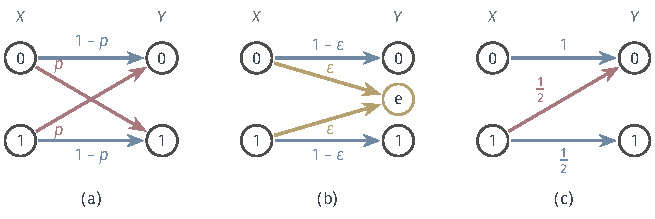
\includegraphics[width=110.9mm]{figures/07-probability/06-channel-coding/tikz/dcc-channel-diagrams/figure.pdf}
 \caption{三个二元输入信道的转移图，箭头上的数是条件概率$W(y\mid x)$。(a) 二元对称信道，红色箭头表示翻转；(b) 二元擦除信道，黄色箭头通向接收端可见的擦除符号$\mathrm{e}$；(c) 本章所用的Z信道，输入$1$以概率$\tfrac12$变成$0$。}
 \label{fig:dcc-channel-diagrams}
\end{BookInlineFigure}

把这些例子的共同结构抽出来：有限的输入字母表、有限的输出字母表，以及每个输入对应的一张输出概率表。

\begin{definition}[离散信道]
\label{def:dcc-channel}
设$\mathcal{X}$、$\mathcal{Y}$是有限集。一个从$\mathcal{X}$到$\mathcal{Y}$的离散信道由一族非负数$W(y\mid x)$给出（$x\in\mathcal{X}$，$y\in\mathcal{Y}$），满足
\begin{equation}
 \sum_{y\in\mathcal{Y}}W(y\mid x)=1,\qquad x\in\mathcal{X} .
 \label{eq:dcc-channel-rows}
\end{equation}
$W(y\mid x)$是输入为$x$时输出为$y$的概率。把它排成$\lvert\mathcal{X}\rvert\times\lvert\mathcal{Y}\rvert$矩阵$\bm{W}$，第$x$行记为$W_x=W(\cdot\mid x)$，称$\bm{W}$为信道的转移矩阵。
\end{definition}

条件~\eqref{eq:dcc-channel-rows}说每一行都是$\mathcal{Y}$上的概率分布。用第~\ref{chap:conditional-distributions}章的语言，$\bm{W}$就是给定$X$时$Y$的条件分布，即一个从$\mathcal{X}$到$\mathcal{Y}$的核；有限字母表上，核就是一张行和为$1$的表。三个例子的转移矩阵依次为
\[
 \begin{pmatrix}1-p&p\\ p&1-p\end{pmatrix},\qquad
 \begin{pmatrix}1-\varepsilon&\varepsilon&0\\ 0&\varepsilon&1-\varepsilon\end{pmatrix},\qquad
 \begin{pmatrix}1&0\\ \tfrac12&\tfrac12\end{pmatrix},
\]
擦除信道的列按输出$0,\mathrm{e},1$排列。

\paragraph{信道固定，输入分布可选}
信道规定的只是“给定输入后输出怎样分布”，至于各个输入多常被使用，由发送端决定。设输入$X$的分布为$q$，即$q(x)=\mathbb{P}(X=x)$，$q$是概率单纯形
\[
 \Delta_{\mathcal{X}}=\Bigl\{q\in\mathbb{R}^{\mathcal{X}}:\ q(x)\geq0,\ \sum_{x}q(x)=1\Bigr\}
\]
中的一点。输入分布与信道合起来确定$(X,Y)$的联合分布与输出分布：
\begin{equation}
 \mathbb{P}(X=x,Y=y)=q(x)W(y\mid x),\qquad
 p_q(y)=\sum_{x\in\mathcal{X}}q(x)W(y\mid x) .
 \label{eq:dcc-output-law}
\end{equation}
写成行向量，$p_q=q\bm{W}$。改变$q$不改变信道，只改变我们如何使用它；后面的容量正是对$q$的最优选择。

式~\eqref{eq:dcc-output-law}说明，输出分布是转移矩阵各行以$q(x)$为权的凸组合。图~\ref{fig:dcc-output-simplex}在输出单纯形中画出这一点。擦除信道$\varepsilon=0.25$的两行是$W_0=(0.75,0.25,0)$与$W_1=(0,0.25,0.75)$，选择$q$只能在连接两行的线段上移动；均匀输入给出中点
\[
 p_q=\tfrac12W_0+\tfrac12W_1=(0.375,\ 0.25,\ 0.375) .
\]
无论怎样选输入，擦除的概率始终是$0.25$：它是信道的性质，输入分布无法改变。

\begin{BookInlineFigure}
 \centering
 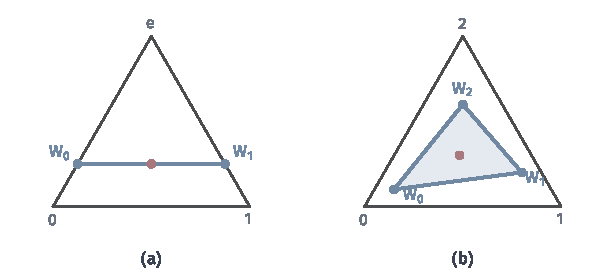
\includegraphics[width=104mm]{figures/07-probability/06-channel-coding/matplotlib/dcc-output-simplex/figure.pdf}
 \caption{输出分布的可达范围。三角形是三个输出上的概率单纯形，顶点是集中于单个输出的分布。(a) 二元擦除信道$\varepsilon=0.25$，蓝点是转移矩阵的两行，蓝线段是$q\bm{W}$的全部可能值；(b) 一个三输入三输出信道，三行为$(0.8,0.1,0.1)$、$(0.1,0.7,0.2)$、$(0.2,0.2,0.6)$，可达的输出分布是浅蓝三角形。红点是均匀输入对应的输出分布。}
 \label{fig:dcc-output-simplex}
\end{BookInlineFigure}

\paragraph{多次使用：无记忆}
传输消息时信道被使用$n$次，输入块$x^n=(x_1,\dots,x_n)$，输出块$y^n=(y_1,\dots,y_n)$。最简单的多次使用规律是：每次使用都经过同一个转移矩阵，各次之间互不影响。

\begin{definition}[离散无记忆信道]
\label{def:dcc-dmc}
以$\bm{W}$为转移矩阵的\term{离散无记忆信道}（discrete memoryless channel）在$n$次使用中，对每个输入块$x^n\in\mathcal{X}^n$，输出块的条件概率为
\begin{equation}
 W^n(y^n\mid x^n)=\prod_{i=1}^{n}W(y_i\mid x_i),\qquad y^n\in\mathcal{Y}^n .
 \label{eq:dcc-memoryless}
\end{equation}
\end{definition}

乘积形式包含两层意思：第$i$个输出只受第$i$个输入影响；给定整个输入块后，各个输出相互独立。以$p=0.1$的二元对称信道为例，发送$111$而收到$101$，需要第一、三位不翻转、第二位翻转，概率是
\[
 W^3(101\mid111)=0.9\times0.1\times0.9=0.081 .
\]

\paragraph{编码器不使用反馈}
式~\eqref{eq:dcc-memoryless}描述的是给定输入块之后输出的规律。还需要说明输入块怎样产生。本章中，发送端在传输之前就由消息确定整个输入块，第$i$次的输入不依赖已经收到的$y_1,\dots,y_{i-1}$。若发送端能看到输出（称为反馈），它可以根据前面的结果调整后面的输入，这时$X_i$与此前的噪声相关，式~\eqref{eq:dcc-memoryless}的乘积结构仍描述每一步的转移，但输入与输出的联合规律不再能直接按块写出，第~\ref{sec:dcc-capacity-formula}节的块互信息上界需要另行论证。图~\ref{fig:dcc-block-system}画出本章的传输结构。

\begin{BookInlineFigure}
 \centering
 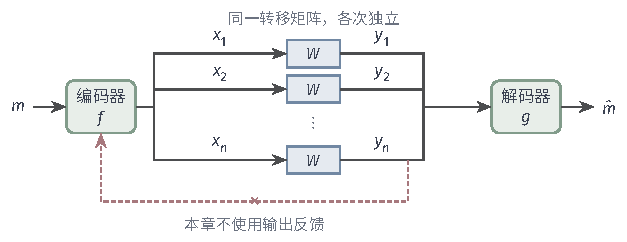
\includegraphics[width=106.2mm]{figures/07-probability/06-channel-coding/tikz/dcc-block-system/figure.pdf}
 \caption{离散无记忆信道上的块传输。编码器$f$把消息$m$一次变成整个输入块，每个符号独立地经过同一转移矩阵$W$，解码器$g$看到整个输出块后给出判决$\hat{m}$。红色虚线表示从输出到编码器的反馈，本章不使用。}
 \label{fig:dcc-block-system}
\end{BookInlineFigure}

无记忆是一个模型假设。若干扰成串出现，例如一次翻转之后紧接着的几个符号也更容易翻转，各次使用就不独立，式~\eqref{eq:dcc-memoryless}不成立。这样的信道需要随机过程的工具描述状态的演化，本章不讨论。


\section{块码}
\label{sec:dcc-block-codes}

一个比特直接送进翻转概率$p=0.1$的二元对称信道，出错的概率就是$0.1$。降低错误的朴素办法是重复：要发$0$就连发$000$，要发$1$就连发$111$，接收端看三个符号中哪个占多数。只有至少两个符号被翻转时才判错，这比单个符号翻转少见得多。

这个例子包含了信道编码的全部要素：消息不是逐个符号送出的，而是先被映成一整块输入；块中的冗余让接收端在部分符号出错时仍能判断发送的是哪条消息。本节把这些要素写成定义，规定码率与错误概率的口径。后面的容量定理和第~\ref{chap:channel-codes}章的具体纠错码都使用这里的口径。

\subsection{编码器与解码器}
\label{sec:dcc-encoder-decoder}

设要传送的消息取自有限集合$\{1,\dots,M\}$，信道使用$n$次。编码就是给每条消息指定一个长度为$n$的输入块，解码就是根据收到的输出块猜出消息。

\begin{definition}[块码]
\label{def:dcc-block-code}
离散信道上的一个$(M,n)$\term{块码}（block code）由两部分组成：
\begin{itemize}
 \item 编码器$f:\{1,\dots,M\}\to\mathcal{X}^n$，记$x^n(m)=f(m)$，称为消息$m$的码字，全部码字组成码本；
 \item 解码器$g:\mathcal{Y}^n\to\{1,\dots,M\}$，把每个输出块判为一条消息。
\end{itemize}
码的码率定义为
\begin{equation}
 R=\frac{\log_2M}{n}\quad\text{比特每次信道使用}.
 \label{eq:dcc-rate}
\end{equation}
\end{definition}

$\log_2M$是从$M$条消息中选出一条所需的比特数，除以$n$就是平均每次使用信道承载的比特数。码率最高为$\log_2\lvert\mathcal{X}\rvert$，此时$M=\lvert\mathcal{X}\rvert^n$，每个输入块都是码字，没有任何冗余。

\paragraph{三次重复码}
\term{重复码}（repetition code）中$M=2$，$n=3$。把消息记作$0$与$1$，码字是$000$与$111$，码率为$\tfrac13$。解码器采用\term{多数判决}（majority decoding）：输出块中$1$多于$0$时判为$1$，否则判为$0$。下面走一遍传输过程，区分四个对象：
\begin{enumerate}
 \item 消息：$m=1$，这是要传的内容；
 \item 码字：$x^3(1)=111$，这是送进信道的输入块；
 \item 输出块：信道翻转了第二位，接收端收到$y^3=101$；
 \item 判决：$101$中有两个$1$，$g(101)=1$，判决$\hat{m}=1$与消息一致。
\end{enumerate}
消息与判决属于消息集合，码字与输出块属于符号块；错误指的是判决与消息不同，而不是输出块与码字不同。这次传输中输出块有一位错了，判决仍然正确。

图~\ref{fig:dcc-repetition-cube}把长度为$3$的全部$8$个输出块画成立方体的顶点，相邻顶点只差一位。两个码字在相对的两个角上，多数判决把立方体分成两半：离$000$较近的四个顶点判为$0$，离$111$较近的四个判为$1$。从$111$出发翻转一位只能走到黄色顶点，所以单个翻转总能被纠正。

\begin{BookInlineFigure}
 \centering
 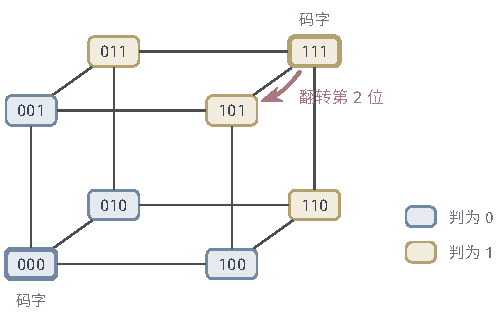
\includegraphics[width=85.4mm]{figures/07-probability/06-channel-coding/tikz/dcc-repetition-cube/figure.pdf}
 \caption{长度为$3$的输出块构成立方体的顶点，相邻顶点只差一位。粗框为码字$000$与$111$；蓝色顶点（至多一个$1$）判为$0$，黄色顶点（至少两个$1$）判为$1$。红色箭头是正文的例子：发送$111$，第二位翻转，收到$101$，判为$1$。}
 \label{fig:dcc-repetition-cube}
\end{BookInlineFigure}

在翻转概率$p=0.1$的二元对称信道上，发送$111$而判错，需要至少两位翻转。恰好两位翻转有$3$种位置，三位全翻有$1$种，所以
\[
 \mathbb{P}(\text{判错})=3p^2(1-p)+p^3=3\times0.01\times0.9+0.001=0.028 .
\]
由对称性，发送$000$时判错的概率也是$0.028$。

\paragraph{最好的解码器}
码本给定以后，解码器还可以自由选择。若每条消息以相同的概率$1/M$出现，判对的概率是
\[
 \frac1M\sum_{m=1}^{M}\ \sum_{y^n:\,g(y^n)=m}W^n\bigl(y^n\mid x^n(m)\bigr)
 =\frac1M\sum_{y^n\in\mathcal{Y}^n}W^n\bigl(y^n\mid x^n(g(y^n))\bigr) .
\]
右边对每个输出块分别求和，因此逐项取最大即可：对每个$y^n$，让$g(y^n)$取使$W^n(y^n\mid x^n(m))$最大的$m$（并列时任取其一）。这样的判决规则称为\term{最大似然解码}（maximum-likelihood decoding），它使均匀消息下的错误概率最小。在$p<\tfrac12$的二元对称信道上，$W^n(y^n\mid x^n)=p^{k}(1-p)^{n-k}$，其中$k$是$y^n$与$x^n$不同的位置数；因为$p/(1-p)<1$，似然随$k$增大而减小，最大似然就是选与输出块差异位置最少的码字。对重复码，这正是多数判决。

\subsection{错误概率与可达速率}
\label{sec:dcc-error-and-rates}

重复码的例子已经给出一个错误概率，但一般的码中，不同消息被判错的概率可以不同。为此先对每条消息定义条件错误概率，再用两种方式汇总。

\begin{definition}[错误概率]
\label{def:dcc-error-probabilities}
对$(M,n)$码，消息$m$的条件错误概率是
\begin{equation}
 \lambda_m=\mathbb{P}\bigl(g(Y^n)\neq m\mid X^n=x^n(m)\bigr)=\sum_{y^n:\,g(y^n)\neq m}W^n\bigl(y^n\mid x^n(m)\bigr) .
 \label{eq:dcc-lambda}
\end{equation}
\term{平均错误概率}（average error probability）与\term{最大错误概率}（maximal error probability）分别为
\begin{equation}
 P_{\mathrm{e}}=\frac1M\sum_{m=1}^{M}\lambda_m,\qquad \lambda_{\max}=\max_{1\leq m\leq M}\lambda_m .
 \label{eq:dcc-pe}
\end{equation}
\end{definition}

若消息$M$在$\{1,\dots,M\}$上均匀分布，$P_{\mathrm{e}}$就是判错的概率$\mathbb{P}(g(Y^n)\neq M)$。这里用同一字母$M$表示消息变量和消息个数，下文由上下文区分。$\lambda_{\max}$不依赖消息的分布，它保证每条消息都很少出错。平均不超过最大值，所以$P_{\mathrm{e}}\leq\lambda_{\max}$；第~\ref{sec:dcc-max-error}小节会说明，在渐近意义下两种口径给出相同的速率极限。

\paragraph{可达速率}
在二元对称信道这类每个输出块都可能来自任一码字的信道上，有限码的错误概率总是正的，所以“可靠”只能在码长增长的极限中定义：要求一列码的错误趋于零，同时码率不低于给定的值。

\begin{definition}[可达速率与容量]
\label{def:dcc-achievable}
称$R\geq0$为\term{可达速率}（achievable rate），若存在一列$(M_n,n)$码，满足
\begin{equation}
 M_n\geq2^{nR},\qquad \lim_{n\to\infty}P_{\mathrm{e}}^{(n)}=0 ,
 \label{eq:dcc-achievable}
\end{equation}
其中$P_{\mathrm{e}}^{(n)}$是第$n$个码的平均错误概率。可达速率的上确界称为信道的\term{信道容量}（channel capacity），记作$C_{\mathrm{op}}$。
\end{definition}

$R=0$总是可达的：取$M_n=1$，只有一条消息，解码器永远判对。可达速率的集合是区间：若$R$可达，比它小的速率用同一列码即可满足$M_n\geq2^{nR'}$。下标“op”表示这个容量是按传输任务定义的；下一节给出一个由信道直接计算的量，第~\ref{sec:dcc-coding-theorem}节证明二者相等。

\paragraph{重复码不够}
长度为奇数$n$的重复码在$p=0.1$的二元对称信道上，判错的概率是$\mathrm{Bin}(n,0.1)$至少取到$(n+1)/2$的概率。由第~\ref{chap:laws-of-large-numbers}章的弱大数律，翻转比例趋于$0.1<\tfrac12$，这个概率趋于零。可是码率$1/n$也趋于零，所以重复码只说明速率$0$可达。图~\ref{fig:dcc-repetition-error}画出前几个重复码：错误按指数下降，但它们在码率—错误平面上全部挤向纵轴，远离$C\approx0.531$。

\begin{BookInlineFigure}
 \centering
 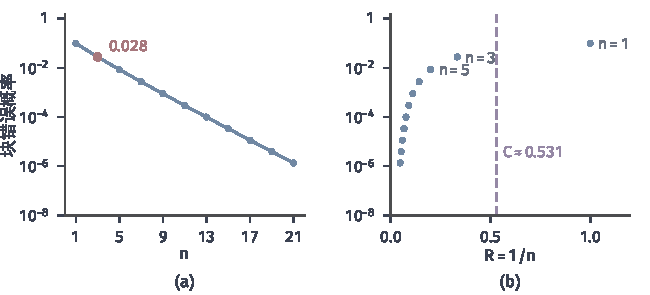
\includegraphics[width=110mm]{figures/07-probability/06-channel-coding/matplotlib/dcc-repetition-error/figure.pdf}
 \caption{翻转概率$0.1$的二元对称信道上，奇数长度$n$的重复码配合多数判决。(a) 块错误概率随$n$的精确值，对数坐标，红点为$n=3$时的$0.028$；(b) 同一组码在码率—错误平面上的位置，码率为$1/n$，紫色虚线为第~\ref{sec:dcc-bsc}小节算出的容量$0.531$。}
 \label{fig:dcc-repetition-error}
\end{BookInlineFigure}

图中$n=1$的“码”码率为$1$，超过了容量，错误概率却只有$0.1$。这并不矛盾：容量限制的是错误能否趋于零，对单个有限码的错误概率没有直接要求。反过来也一样，速率低于容量只保证存在错误趋于零的码列，并不保证某个有限长度的码错误为零。可达速率是关于码长增长时的极限陈述，有限长度需要多少冗余由第~\ref{chap:channel-codes}章讨论。


\section{容量公式}
\label{sec:dcc-capacity-formula}

可达速率的定义涉及所有码长、所有码本与所有解码器，直接求其上确界无从下手。本节从信道本身构造一个可以计算的量，并证明它控制任意长度输入块能获得的信息。下一节再证明它就是$C_{\mathrm{op}}$。

\paragraph{计数的图景}
先用一个粗略的计数说明为什么应当看互信息。设输入块的各符号按分布$q$独立选取，输出块也就按$p_q$独立分布。由第~\ref{chap:lossless-coding}章的典型集合，输出块几乎总落在约$2^{nH(Y)}$个“典型”输出块之中；给定一个码字，信道噪声使输出块落在约$2^{nH(Y\mid X)}$个块组成的小范围内。若要从输出块唯一认出码字，各码字的小范围应当基本不重叠，于是码字数至多约为
\[
 \frac{2^{nH(Y)}}{2^{nH(Y\mid X)}}=2^{n\,(H(Y)-H(Y\mid X))}=2^{nI(X;Y)} .
\]
每次使用约承载$I(X;Y)$比特。图~\ref{fig:dcc-typical-fans}画出这幅图景。它是启发，不是证明：“约”字隐去了误差，小范围之间也不必完全不交。第~\ref{sec:dcc-coding-theorem}节把这个计数做成严格的论证。

\begin{BookInlineFigure}
 \centering
 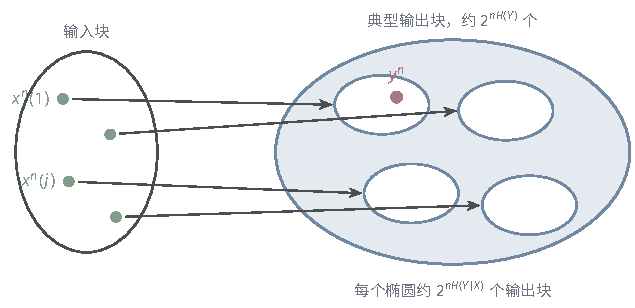
\includegraphics[width=107.5mm]{figures/07-probability/06-channel-coding/tikz/dcc-typical-fans/figure.pdf}
 \caption{容量公式背后的计数。左侧绿点是按输入分布选出的码字；右侧蓝色区域是约$2^{nH(Y)}$个典型输出块，每个码字经过信道后的可能输出集中在约$2^{nH(Y\mid X)}$个块组成的小椭圆中。红点是收到的输出块，它落在所发码字的椭圆内。互不重叠的椭圆至多约有$2^{nI(X;Y)}$个。}
 \label{fig:dcc-typical-fans}
\end{BookInlineFigure}

\paragraph{互信息作为输入分布的函数}
固定信道$\bm{W}$，输入分布为$q$时，第~\ref{chap:information-measures}章的互信息（以比特计）是
\[
 I(X;Y)=\sum_{x,y}q(x)W(y\mid x)\log_2\frac{W(y\mid x)}{p_q(y)} ,
\]
求和只取$q(x)W(y\mid x)>0$的项，此时$p_q(y)\geq q(x)W(y\mid x)>0$，每项都有定义。字母表有限，所以各个熵都有限，并且$I(X;Y)=H(Y)-H(Y\mid X)$。按输入分组，内层和正是第$x$行相对于输出分布的KL散度，于是
\begin{equation}
 I(q)=\sum_{x\in\mathcal{X}}q(x)\,D_{\mathrm{KL}}\bigl(W_x\Vert p_q\bigr) .
 \label{eq:dcc-mi-divergence}
\end{equation}
这里把互信息写成$I(q)$，强调信道固定后它只是$q$的函数。式~\eqref{eq:dcc-mi-divergence}的读法是：每个输入$x$的输出分布偏离总体输出分布越远，用$x$传递的信息越多；互信息是这些偏离按使用频率的平均。

\begin{definition}[信息容量]
\label{def:dcc-information-capacity}
离散信道$\bm{W}$的信息容量是
\begin{equation}
 C=\max_{q\in\Delta_{\mathcal{X}}}I(q) .
 \label{eq:dcc-capacity}
\end{equation}
达到最大值的$q$称为最优输入分布。
\end{definition}

定义中写的是最大值而不是上确界，需要说明它能取到；同时，最优输入分布怎样刻画，也决定了后面的计算方法。

\begin{theorem}[容量的存在与凹性]
\label{thm:dcc-capacity-exists}
$I(q)$是单纯形$\Delta_{\mathcal{X}}$上的连续凹函数。因此式~\eqref{eq:dcc-capacity}的最大值存在，并且
\begin{equation}
 0\leq C\leq\min\bigl\{\log_2\lvert\mathcal{X}\rvert,\ \log_2\lvert\mathcal{Y}\rvert\bigr\} ;
 \label{eq:dcc-capacity-range}
\end{equation}
最优输入分布组成凸集，所有最优输入分布给出同一个输出分布。
\end{theorem}

\begin{proof}
把互信息写成熵差：
\[
 I(q)=H(p_q)-\sum_{x}q(x)H(W_x) ,
\]
其中$H(p_q)=\sum_y\varphi(p_q(y))$，$\varphi(t)=-t\log_2t$（$\varphi(0)=0$）。$\varphi$在$[0,1]$上连续，$p_q$是$q$的线性函数，所以$H(p_q)$关于$q$连续；第二项是$q$的线性函数。于是$I$连续。

凹性。第~\ref{chap:information-measures}章证明了熵是概率分布的凹函数，而且因为$\varphi$严格凹，这种凹性是严格的：$p\neq p'$时，对$0<\theta<1$有$H(\theta p+(1-\theta)p')>\theta H(p)+(1-\theta)H(p')$。$q\mapsto p_q$是线性的，凹函数与线性映射的复合仍是凹函数；减去一个线性函数不改变凹性。所以$I$凹。

$\Delta_{\mathcal{X}}$是有界闭集，连续函数在其上取到最大值。凹函数在凸集上的最大值点组成凸集：若$q_1,q_2$都达到$C$，则对$\theta\in[0,1]$，
\[
 I\bigl(\theta q_1+(1-\theta)q_2\bigr)\geq\theta C+(1-\theta)C=C .
\]
若两者的输出分布不同，由$H$的严格凹性，中点处的不等式是严格的，$I$会超过$C$，这不可能。所以最优输出分布唯一。

上界：$I(X;Y)\leq H(X)\leq\log_2\lvert\mathcal{X}\rvert$，同理$I(X;Y)\leq H(Y)\leq\log_2\lvert\mathcal{Y}\rvert$；下界由互信息非负得到。
\end{proof}

凹性带来的好处是局部最优就是全局最优，最优输入可以用一阶条件刻画。凹性本身不保证最优输入唯一：例如两个输入的转移行完全相同时，它们之间的分配可以任意调换。

\paragraph{例：Z信道}
Z信道中记$q=\mathbb{P}(X=1)$。输出为$1$当且仅当输入为$1$且没有出错，所以$p_q(1)=q/2$。给定$X=0$时输出确定，熵为$0$；给定$X=1$时输出是公平硬币，熵为$1$比特。于是
\[
 I(q)=h_2\Bigl(\frac q2\Bigr)-q ,
\]
其中$h_2(t)=-t\log_2t-(1-t)\log_2(1-t)$是二元熵函数。对$q$求导，$h_2'(t)=\log_2\frac{1-t}{t}$，得到
\[
 I'(q)=\frac12\log_2\frac{2-q}{q}-1 .
\]
令它为零，得$(2-q)/q=4$，即$q=\tfrac25$。代回，$h_2(\tfrac15)=\log_25-\tfrac85$，所以
\[
 C=\log_25-\frac85-\frac25=\log_2\frac54\approx0.3219 .
\]
最优输入并不均匀：输入$1$会以一半的概率被误读成$0$，少用一些更划算。均匀输入时$I(\tfrac12)=h_2(\tfrac14)-\tfrac12\approx0.3113$，比容量少约$0.011$比特。图~\ref{fig:dcc-mi-curves}把它与两个对称信道的$I(q)$画在一起。

\begin{BookInlineFigure}
 \centering
 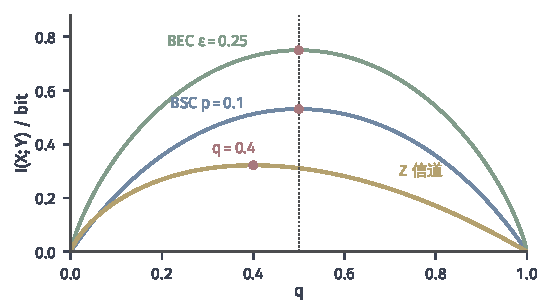
\includegraphics[width=92mm]{figures/07-probability/06-channel-coding/matplotlib/dcc-mi-curves/figure.pdf}
 \caption{三个二元输入信道的互信息随输入概率$q=\mathbb{P}(X=1)$的变化：蓝线为翻转概率$0.1$的二元对称信道，绿线为擦除概率$0.25$的二元擦除信道，黄线为Z信道。三条曲线都是凹的，红点为最大值即容量；两个对称信道在$q=\tfrac12$处取最大值，Z信道在$q=0.4$处取最大值$\log_2(5/4)$。}
 \label{fig:dcc-mi-curves}
\end{BookInlineFigure}

\paragraph{最优性条件}
对二元输入，一元求导就能找到最大值；输入多于两个时，需要一个对单纯形上的点都适用的判别法。式~\eqref{eq:dcc-mi-divergence}提示：最优时，凡是被使用的输入，其“信息贡献”$D_{\mathrm{KL}}(W_x\Vert p_q)$应当相等，否则把概率从贡献小的输入挪到贡献大的输入就能增加互信息。下面的定理把这一想法写准确，并顺带给出一个任何时候都能算的上界。

\begin{theorem}[容量的上界与最优性条件]
\label{thm:dcc-kkt}
\begin{enumerate}
 \item 对$\mathcal{Y}$上的任意概率分布$r$，
 \begin{equation}
  C\leq\max_{x\in\mathcal{X}}D_{\mathrm{KL}}\bigl(W_x\Vert r\bigr) .
  \label{eq:dcc-upper-bound}
 \end{equation}
 \item $q^{*}\in\Delta_{\mathcal{X}}$是最优输入分布，当且仅当存在常数$c$，使得记$p^{*}=p_{q^{*}}$时
 \begin{equation}
  D_{\mathrm{KL}}\bigl(W_x\Vert p^{*}\bigr)=c\ \ \text{若}\ q^{*}(x)>0,\qquad D_{\mathrm{KL}}\bigl(W_x\Vert p^{*}\bigr)\leq c\ \ \text{若}\ q^{*}(x)=0 .
  \label{eq:dcc-kkt}
 \end{equation}
 此时$c=C$。
\end{enumerate}
\end{theorem}

\begin{proof}
先证一个恒等式。对任意$q$与任意$r$，把$\log_2(W/r)$拆成$\log_2(W/p_q)+\log_2(p_q/r)$，得到
\[
 \sum_{x}q(x)D_{\mathrm{KL}}(W_x\Vert r)=\sum_xq(x)D_{\mathrm{KL}}(W_x\Vert p_q)+\sum_{y}p_q(y)\log_2\frac{p_q(y)}{r(y)} ,
\]
其中用到$\sum_xq(x)W(y\mid x)=p_q(y)$。由式~\eqref{eq:dcc-mi-divergence}，右边是$I(q)+D_{\mathrm{KL}}(p_q\Vert r)$。若某项为无穷，等式两边同为无穷。于是
\[
 I(q)=\sum_xq(x)D_{\mathrm{KL}}(W_x\Vert r)-D_{\mathrm{KL}}(p_q\Vert r)\leq\max_xD_{\mathrm{KL}}(W_x\Vert r) .
\]
对$q$取最大值就得到式~\eqref{eq:dcc-upper-bound}。

充分性。设式~\eqref{eq:dcc-kkt}成立。由式~\eqref{eq:dcc-mi-divergence}，$I(q^{*})$是$D_{\mathrm{KL}}(W_x\Vert p^{*})$在$q^{*}$支撑上的平均，等于$c$。取$r=p^{*}$，式~\eqref{eq:dcc-upper-bound}给出$C\leq c$。所以$I(q^{*})=c\geq C$，$q^{*}$最优且$c=C$。

必要性。设$q^{*}$最优，任取$x'\in\mathcal{X}$，令$q_t=(1-t)q^{*}+t\,\delta_{x'}$，$t\in[0,1]$，其中$\delta_{x'}$是集中在$x'$的分布。先设$W_{x'}$的支撑包含在$p^{*}$的支撑中。对$I(q_t)=H(p_{q_t})-\sum_xq_t(x)H(W_x)$在$t=0$处求右导数，$p_{q_t}=p^{*}+t(W_{x'}-p^{*})$，熵项的导数是
\[
 \begin{aligned}
 &-\sum_{y}\bigl(W(y\mid x')-p^{*}(y)\bigr)\Bigl(\log_2p^{*}(y)+\frac{1}{\ln2}\Bigr)\\
 &\qquad=-\sum_yW(y\mid x')\log_2p^{*}(y)-H(p^{*}) ,
 \end{aligned}
\]
这里只对$p^{*}(y)>0$的$y$求和，$\sum_y(W(y\mid x')-p^{*}(y))=0$消去了常数项。线性项的导数是$-H(W_{x'})+\sum_xq^{*}(x)H(W_x)$。两部分相加，得到
\[
 \frac{\mathrm{d}}{\mathrm{d}t}I(q_t)\Big|_{t=0^{+}}=D_{\mathrm{KL}}(W_{x'}\Vert p^{*})-I(q^{*}) .
\]
$q^{*}$是最大值点，右导数不能为正，所以$D_{\mathrm{KL}}(W_{x'}\Vert p^{*})\leq I(q^{*})=C$。若$W_{x'}$在某个$p^{*}(y)=0$的$y$上有正质量，则$p_{q_t}(y)=tW(y\mid x')$，熵中这一项$-tW\log_2(tW)$的右导数为$+\infty$，其余项导数有限，$I(q_t)$在$t=0$附近严格增加，与最优性矛盾；所以这种情形不会出现。于是对一切$x'$有$D_{\mathrm{KL}}(W_{x'}\Vert p^{*})\leq C$；而这些散度按$q^{*}$的平均等于$C$，所以在支撑上必须取等号。
\end{proof}

式~\eqref{eq:dcc-kkt}是卷五中约束优化一阶条件在单纯形上的具体形式：等式约束$\sum_xq(x)=1$的乘子是$c$，非负约束在$q^{*}(x)=0$处起作用，允许不等号，可参考\BookChapterRef{chap:constrained-optimality}{卷五第17章“约束问题的最优性”}。上界~\eqref{eq:dcc-upper-bound}对任意$r$成立，不需要知道最优输入；第~\ref{sec:dcc-numerical}节用它作为数值计算的停止依据。

用Z信道检验条件~\eqref{eq:dcc-kkt}。$q^{*}=(\tfrac35,\tfrac25)$时$p^{*}=(\tfrac45,\tfrac15)$，两行的散度为
\[
 \begin{aligned}
 D_{\mathrm{KL}}(W_0\Vert p^{*})&=\log_2\frac{1}{4/5}=\log_2\frac54 ,\\
 D_{\mathrm{KL}}(W_1\Vert p^{*})&=\frac12\log_2\frac{1/2}{4/5}+\frac12\log_2\frac{1/2}{1/5}=\frac12\log_2\frac{25}{16}=\log_2\frac54 .
 \end{aligned}
\]
两者相等，都等于容量。

\paragraph{块的互信息不超过单次容量的$n$倍}
容量是单次使用的量，传输却用整块输入。块输入的各符号可以按任意方式相关，例如重复码让三个符号完全相同。这种相关能否让$n$次使用获得多于$nC$的信息？下面的引理说不能，并且独立使用最优输入恰好达到$nC$。

\begin{lemma}[块互信息的单次上界]
\label{lem:dcc-block-bound}
设$X^n=(X_1,\dots,X_n)$在$\mathcal{X}^n$上有任意分布，给定$X^n=x^n$时$Y^n$的条件分布由式~\eqref{eq:dcc-memoryless}给出。则
\begin{equation}
 I(X^n;Y^n)\leq\sum_{i=1}^{n}I(X_i;Y_i)\leq nC .
 \label{eq:dcc-block-bound}
\end{equation}
若$X_1,\dots,X_n$独立且都服从最优输入分布，则两处都取等号。
\end{lemma}

\begin{proof}
先算条件熵。对式~\eqref{eq:dcc-memoryless}中$j\neq i$的坐标求和，每个因子$\sum_{y_j}W(y_j\mid x_j)=1$，得到$\mathbb{P}(Y_i=y\mid X^n=x^n)=W(y\mid x_i)$：$(X_i,Y_i)$的联合分布是$X_i$的边缘分布乘以$\bm{W}$。取对数，乘积变成和：
\[
 \begin{aligned}
 H(Y^n\mid X^n)&=\mathbb{E}\bigl[-\log_2W^n(Y^n\mid X^n)\bigr]\\
 &=\sum_{i=1}^{n}\mathbb{E}\bigl[-\log_2W(Y_i\mid X_i)\bigr]=\sum_{i=1}^{n}H(Y_i\mid X_i) .
 \end{aligned}
\]
再看输出熵。由熵的链式法则与“条件化不增加熵”，
\[
 H(Y^n)=\sum_{i=1}^{n}H(Y_i\mid Y_1,\dots,Y_{i-1})\leq\sum_{i=1}^{n}H(Y_i) .
\]
两式相减，
\[
 \begin{aligned}
 I(X^n;Y^n)&=H(Y^n)-H(Y^n\mid X^n)\\
 &\leq\sum_{i=1}^{n}\bigl(H(Y_i)-H(Y_i\mid X_i)\bigr)=\sum_{i=1}^{n}I(X_i;Y_i) .
 \end{aligned}
\]
每个$I(X_i;Y_i)$是$X_i$的边缘分布对应的互信息，不超过$C$。

若$X_i$独立同服从最优分布$q^{*}$，则联合概率$\prod_iq^{*}(x_i)W(y_i\mid x_i)$分解为$n$个相同因子的乘积，$(X_i,Y_i)$相互独立，$Y_1,\dots,Y_n$也相互独立，于是$H(Y^n)=\sum_iH(Y_i)$，且每个$I(X_i;Y_i)=C$。
\end{proof}

图~\ref{fig:dcc-memoryless-graph}画出证明所用的依赖结构。条件熵能够精确相加，是因为每个输出只通过自己的输入受影响；输出熵只能放大成和，是因为各输出可能经由输入彼此相关。输入之间的相关只会让$H(Y^n)$变小，不会让信息变多：重复码的三个输出高度相关，所以三次使用得到的信息远少于$3C$。

\begin{BookInlineFigure}
 \centering
 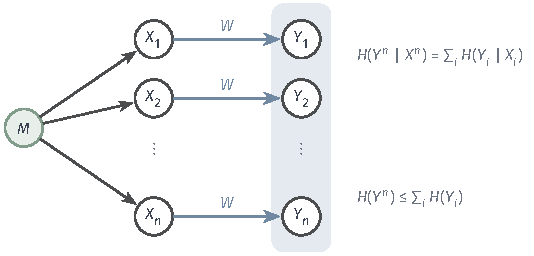
\includegraphics[width=90.5mm]{figures/07-probability/06-channel-coding/tikz/dcc-memoryless-graph/figure.pdf}
 \caption{无反馈块传输的依赖结构。消息$M$决定整个输入块，各输入可以经由$M$相关；每个输出$Y_i$只由$X_i$经过同一个$W$产生。条件熵因此精确相加，而浅蓝色框内的输出可能彼此相关，输出熵只满足次可加不等式。}
 \label{fig:dcc-memoryless-graph}
\end{BookInlineFigure}

引理只说块输入能获得的信息至多为$nC$，还没有说明这些信息能被一个码本和一个解码器实际兑现成低错误的消息传输，也没有说明信息上界为什么限制码率。这两个方向分别是下一节的可达性与逆定理。


\section{信道编码定理}
\label{sec:dcc-coding-theorem}

现在有两个“容量”：按传输任务定义的$C_{\mathrm{op}}$，即错误能趋于零的码率的上确界；以及式~\eqref{eq:dcc-capacity}中由转移矩阵算出的$C$。引理~\ref{lem:dcc-block-bound}说明$n$次使用至多获得$nC$比特信息，计数图景又提示$2^{nC}$条消息大致能被区分。下面的定理说两者相等。

\begin{theorem}[信道编码定理]
\label{thm:dcc-coding-theorem}
对有限字母表上的离散无记忆信道（编码器不使用反馈），
\begin{equation}
 C_{\mathrm{op}}=C=\max_{q\in\Delta_{\mathcal{X}}}I(q) .
 \label{eq:dcc-coding-theorem}
\end{equation}
具体地说：每个$R<C$都是可达速率，并且可以要求最大错误概率趋于零；每个$R>C$都不是可达速率。
\end{theorem}

定理由两个方向组成。可达性（第~\ref{sec:dcc-achievability}小节）是存在性陈述：码率低于容量时，存在错误趋于零的码列。逆定理（第~\ref{sec:dcc-converse}小节）是必要性陈述：码率高于容量时，任何码列的错误都不能趋于零。定理对$R=C$本身不作断言，也不说某个有限长度的码已经可靠；它描述的是码长增长时能够逼近的速率边界。这一陈述最早由Shannon给出，完整的历史与推广可查阅~\scite{math-cover2006information}。

\subsection{随机编码的可达性}
\label{sec:dcc-achievability}

要证明可达，需要对每个$R<C$造出一列码。直接构造很难，证明采用一个间接办法：随机抽取码本，证明随机码本的平均错误概率趋于零，于是必有某个具体码本不比平均差。解码器则用“联合典型性”判断一个码字与输出块是否匹配。

\paragraph{联合典型集}
设$(X,Y)$的联合分布为$q(x)W(y\mid x)$，输出分布为$p=p_q$。把$n$个独立同分布的对$(X_i,Y_i)$排成块，块的概率是单个概率的乘积，记作$q^n(x^n)=\prod_iq(x_i)$，$p^n(y^n)=\prod_ip(y_i)$，以及$P^n(x^n,y^n)=\prod_iq(x_i)W(y_i\mid x_i)$。由第~\ref{chap:laws-of-large-numbers}章的大数律，$-\frac1n\log_2q^n(X^n)$是$n$个独立同分布的$-\log_2q(X_i)$的平均，会集中到它的均值$H(X)$。联合典型集把这种集中同时要求在三个层面上。

\begin{definition}[联合典型集]
\label{def:dcc-joint-typical}
给定$\epsilon>0$，\term{联合典型集}（jointly typical set）$A_{\epsilon}^{(n)}$由满足下面三个条件的$(x^n,y^n)\in\mathcal{X}^n\times\mathcal{Y}^n$组成：
\begin{equation}
 \begin{aligned}
 \Bigl\lvert-\tfrac1n\log_2q^n(x^n)-H(X)\Bigr\rvert&<\epsilon ,\\
 \Bigl\lvert-\tfrac1n\log_2p^n(y^n)-H(Y)\Bigr\rvert&<\epsilon ,\\
 \Bigl\lvert-\tfrac1n\log_2P^n(x^n,y^n)-H(X,Y)\Bigr\rvert&<\epsilon .
 \end{aligned}
 \label{eq:dcc-joint-typical}
\end{equation}
概率为零的块，其负对数视为$+\infty$，不属于$A_{\epsilon}^{(n)}$。
\end{definition}

直观上，联合典型的一对块“看起来像”由这条信道产生的：输入块的组成像$q$，输出块的组成像$p$，两者之间的对应关系像$\bm{W}$。下面的引理给出三条性质，分别对应计数图景中的三个“约”字。

\begin{lemma}[联合典型性]
\label{lem:dcc-joint-aep}
\begin{enumerate}
 \item 若$(X_i,Y_i)$独立同服从$q(x)W(y\mid x)$，则当$n\to\infty$时
 \begin{equation}
  \mathbb{P}\bigl((X^n,Y^n)\in A_{\epsilon}^{(n)}\bigr)\to1 .
  \label{eq:dcc-typical-prob}
 \end{equation}
 \item 典型集的元素个数满足
 \begin{equation}
  \bigl\lvert A_{\epsilon}^{(n)}\bigr\rvert\leq2^{n(H(X,Y)+\epsilon)} .
  \label{eq:dcc-typical-size}
 \end{equation}
 \item 若$\tilde{X}^n\sim q^n$与$\tilde{Y}^n\sim p^n$相互独立，则
 \begin{equation}
  \mathbb{P}\bigl((\tilde{X}^n,\tilde{Y}^n)\in A_{\epsilon}^{(n)}\bigr)\leq2^{-n(I(X;Y)-3\epsilon)} .
  \label{eq:dcc-independent-typical}
 \end{equation}
\end{enumerate}
\end{lemma}

\begin{proof}
(1) 以概率$1$，每个$X_i$取$q(x)>0$的值，每对取正概率的值，所以$-\log_2q(X_i)$、$-\log_2p(Y_i)$、$-\log_2[q(X_i)W(Y_i\mid X_i)]$都是有界的随机变量，均值分别为$H(X)$、$H(Y)$、$H(X,Y)$。块的负对数概率除以$n$恰好是它们的样本平均。由弱大数律，对每个条件，违反它的概率趋于零；三个概率之和也趋于零。

(2) 集合中每一对都满足$P^n(x^n,y^n)\geq2^{-n(H(X,Y)+\epsilon)}$，所以
\[
 1\geq\sum_{(x^n,y^n)\in A_{\epsilon}^{(n)}}P^n(x^n,y^n)\geq\bigl\lvert A_{\epsilon}^{(n)}\bigr\rvert\,2^{-n(H(X,Y)+\epsilon)} .
\]

(3) 独立的一对取值$(x^n,y^n)$的概率是$q^n(x^n)p^n(y^n)$。在$A_{\epsilon}^{(n)}$上，由前两个条件，它不超过$2^{-n(H(X)-\epsilon)}2^{-n(H(Y)-\epsilon)}$。乘以(2)中的个数，
\[
 \mathbb{P}\bigl((\tilde{X}^n,\tilde{Y}^n)\in A_{\epsilon}^{(n)}\bigr)\leq2^{n(H(X,Y)+\epsilon)}\,2^{-n(H(X)+H(Y)-2\epsilon)}=2^{-n(I(X;Y)-3\epsilon)} ,
\]
最后用到$I(X;Y)=H(X)+H(Y)-H(X,Y)$。
\end{proof}

第(1)条说正确的一对几乎总是典型的，第(3)条说无关的一对很少看起来像典型的。两条之间的差距就是解码的依据。图~\ref{fig:dcc-info-density}在翻转概率$0.1$、均匀输入的二元对称信道上画出这一差距。此时$-\frac1n\log_2q^n(x^n)=1=H(X)$对每个块都成立，输出块也一样，三个条件只剩第三个；它等价于看信息密度
\[
 \frac1n\log_2\frac{W^n(y^n\mid x^n)}{p^n(y^n)}=1+\frac kn\log_2p+\Bigl(1-\frac kn\Bigr)\log_2(1-p)
\]
是否接近$I(X;Y)=0.531$，其中$k$是$x^n$与$y^n$不同的位置数。正确的一对中$k\sim\mathrm{Bin}(n,0.1)$；独立的一对中$k\sim\mathrm{Bin}(n,\tfrac12)$，信息密度集中在$-0.737$附近。$n$增大时两团质量都收缩，彼此分离得越来越清楚。

\begin{BookInlineFigure}
 \centering
 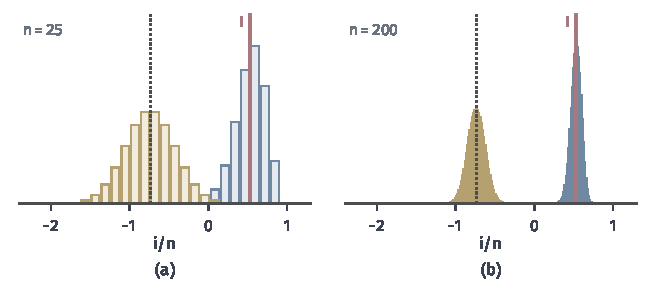
\includegraphics[width=110mm]{figures/07-probability/06-channel-coding/matplotlib/dcc-info-density/figure.pdf}
 \caption{翻转概率$0.1$的二元对称信道、均匀输入时，归一化信息密度$i/n=\frac1n\log_2[W^n(y^n\mid x^n)/p^n(y^n)]$的精确分布。蓝色为码字与其输出块的正确配对，黄色为与输出块独立的码字；红线为$I=0.531$，点线为独立配对的均值$-0.737$。(a) $n=25$；(b) $n=200$。}
 \label{fig:dcc-info-density}
\end{BookInlineFigure}

\paragraph{可达性的证明}

\begin{theorem}[可达性]
\label{thm:dcc-achievability}
对离散无记忆信道，每个$0\leq R<C$都是可达速率。
\end{theorem}

\begin{proof}
$R=0$已知可达，下设$0<R<C$。取最优输入分布$q^{*}$，于是$I(X;Y)=C$；再取$\epsilon>0$使$R<C-3\epsilon$。令$M=\lceil2^{nR}\rceil$，则$M-1<2^{nR}$。

随机码本。独立地抽取$M$个码字$\mathsf{X}^n(1),\dots,\mathsf{X}^n(M)$，每个码字的$n$个符号独立同服从$q^{*}$，即每个码字服从$(q^{*})^n$。码本抽定以后告诉收发双方，传输消息$m$时发送$\mathsf{X}^n(m)$。

解码规则。收到$y^n$后，若恰有一个$\hat{m}$使$(\mathsf{X}^n(\hat{m}),y^n)\in A_{\epsilon}^{(n)}$，就判为$\hat{m}$；否则判为$1$。

错误分析。固定消息$m$，设发送的是$\mathsf{X}^n(m)$，输出为$Y^n$。定义事件
\[
 E_j=\bigl\{(\mathsf{X}^n(j),Y^n)\in A_{\epsilon}^{(n)}\bigr\},\qquad j=1,\dots,M .
\]
若$E_m$发生而其余$E_j$都不发生，解码器判为$m$。所以判错的事件包含于$E_m^{\mathrm{c}}\cup\bigcup_{j\neq m}E_j$，由并集上界，对码本与信道噪声一起取概率，
\[
 \mathbb{E}[\lambda_m]\leq\mathbb{P}(E_m^{\mathrm{c}})+\sum_{j\neq m}\mathbb{P}(E_j) ,
\]
这里$\lambda_m$随码本而变，$\mathbb{E}$是对码本求平均。

第一项：$(\mathsf{X}^n(m),Y^n)$的各对$(X_i,Y_i)$独立同服从$q^{*}(x)W(y\mid x)$，由引理~\ref{lem:dcc-joint-aep}(1)，$\mathbb{P}(E_m^{\mathrm{c}})\to0$。

第二项：$j\neq m$时，$\mathsf{X}^n(j)$与$(\mathsf{X}^n(m),Y^n)$独立，而$Y^n$的边缘分布是$(p^{*})^n$。由式~\eqref{eq:dcc-independent-typical}，$\mathbb{P}(E_j)\leq2^{-n(C-3\epsilon)}$。合起来，
\[
 \mathbb{E}[\lambda_m]\leq\mathbb{P}(E_m^{\mathrm{c}})+(M-1)\,2^{-n(C-3\epsilon)}\leq\mathbb{P}(E_m^{\mathrm{c}})+2^{-n(C-3\epsilon-R)} .
\]
右边与$m$无关，记为$\delta_n$；因为$C-3\epsilon-R>0$，$\delta_n\to0$。

选出确定码本。对$m$取平均，随机码本的平均错误概率满足$\mathbb{E}[P_{\mathrm{e}}]\leq\delta_n$。一个随机变量不可能处处大于它的均值，所以存在某个具体码本，其平均错误概率$P_{\mathrm{e}}^{(n)}\leq\delta_n$。对每个$n$取这样一个码本，得到$M_n=\lceil2^{nR}\rceil\geq2^{nR}$且$P_{\mathrm{e}}^{(n)}\to0$的码列。
\end{proof}

为什么码率低于互信息就够了？错误有两个来源。正确码字不典型，这由大数律控制，与码率无关。某个竞争码字碰巧看起来与输出匹配，每个竞争者的机会约为$2^{-nC}$，竞争者约有$2^{nR}$个，总机会约为$2^{-n(C-R)}$；只要$R<C$，它就按指数趋于零。这正是计数图景的严格版本：小椭圆的个数$2^{nR}$少于能容纳的数目$2^{nC}$。

\paragraph{一个精确的数值}
在翻转概率$0.1$、均匀输入的二元对称信道上，证明中的两项都可以按$k$的二项分布精确求和，不必用指数上界。图~\ref{fig:dcc-random-coding-bound}画出$\mathbb{P}(E_m^{\mathrm{c}})+(M-1)\mathbb{P}(E_j)$随块长的变化（在$1$处截断），容差取$\epsilon=(C-R)/2$。$R=0.25$时，$n=1000$的值约为$4.7\times10^{-6}$，$n=2000$时约为$2.2\times10^{-10}$；$R=0.40$更靠近容量，$n=1000$时仍有$0.031$，$n=2000$时降到$0.0020$。越靠近容量，需要的块长越长。$R=0.60$高于容量，这个上界始终为$1$；下一小节证明这不只是上界的缺陷。

\begin{BookInlineFigure}
 \centering
 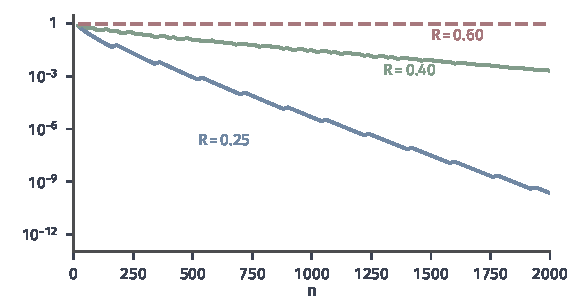
\includegraphics[width=96mm]{figures/07-probability/06-channel-coding/matplotlib/dcc-random-coding-bound/figure.pdf}
 \caption{翻转概率$0.1$的二元对称信道上随机编码的错误上界$\mathbb{P}(E_m^{\mathrm{c}})+(M-1)\mathbb{P}(E_j)$，$M=\lceil2^{nR}\rceil$，均匀输入，两项都按二项分布精确计算，值在$1$处截断，纵轴为对数坐标。蓝线$R=0.25$与绿线$R=0.40$低于容量$0.531$，容差$\epsilon=(C-R)/2$；红色虚线$R=0.60$高于容量，取$\epsilon=0.05$。曲线的小幅锯齿来自$k$的整数取值。}
 \label{fig:dcc-random-coding-bound}
\end{BookInlineFigure}

\paragraph{存在不等于可用}
证明只说明好码本存在，没有给出低成本的编码与解码。随机码本没有结构，必须整体存储$M n$个符号；典型性解码要把输出块与全部$M$个码字逐一比较。$R=0.25$、$n=1000$时，$M=2^{250}$，无论存储还是比较都无法实现。用代数结构降低编码与解码的代价，是第~\ref{chap:channel-codes}章的任务。

\subsection{逆定理}
\label{sec:dcc-converse}

可达性给出了容量以下的速率。反方向要说明：码率高于$C$时，无论码本与解码器如何设计，错误都不能趋于零。思路是把“判对”翻译成“消息与输出之间有很多信息”，再用引理~\ref{lem:dcc-block-bound}说明信息不会超过$nC$。

翻译所用的工具是第~\ref{chap:information-measures}章的Fano不等式。设消息变量取值于$M\geq2$个标签，$\hat{M}$是对它的判决，$P_{\mathrm{e}}=\mathbb{P}(\hat{M}\neq M)$。以比特计，Fano不等式为
\[
 H(M\mid\hat{M})\leq h_2(P_{\mathrm{e}})+P_{\mathrm{e}}\log_2(M-1)\leq1+P_{\mathrm{e}}\log_2M ,
\]
第二步用了$h_2\leq1$。它说判错的机会小，判决后剩余的不确定性就少。

\begin{theorem}[逆定理]
\label{thm:dcc-converse}
设$(M,n)$码用于离散无记忆信道，编码器不使用反馈，$M\geq2$，消息均匀分布。则平均错误概率满足
\begin{equation}
 P_{\mathrm{e}}\geq1-\frac{nC+1}{\log_2M} .
 \label{eq:dcc-fano-bound}
\end{equation}
特别地，若$M\geq2^{nR}$，则$P_{\mathrm{e}}\geq1-C/R-1/(nR)$；当$R>C$时，任何这样的码列都满足
\begin{equation}
 \liminf_{n\to\infty}P_{\mathrm{e}}^{(n)}\geq1-\frac CR>0 ,
 \label{eq:dcc-weak-converse}
\end{equation}
所以$R$不可达。
\end{theorem}

\begin{proof}
消息均匀，$H(M)=\log_2M$。按条件熵与互信息的关系，
\[
 \log_2M=H(M\mid\hat{M})+I(M;\hat{M}) .
\]
第一项用Fano不等式：$H(M\mid\hat{M})\leq1+P_{\mathrm{e}}\log_2M$。

第二项用数据处理不等式两次。判决$\hat{M}=g(Y^n)$只依赖输出块，所以$I(M;\hat{M})\leq I(M;Y^n)$。码字$X^n=f(M)$由消息决定，而且因为没有反馈，给定$X^n$后$Y^n$的条件分布由式~\eqref{eq:dcc-memoryless}决定，不再依赖$M$：$M$、$X^n$、$Y^n$按顺序构成Markov链，于是$I(M;Y^n)\leq I(X^n;Y^n)$。再由引理~\ref{lem:dcc-block-bound}，
\[
 I(M;\hat{M})\leq I(X^n;Y^n)\leq nC .
\]

两项相加，得到
\[
 \log_2M\leq1+P_{\mathrm{e}}\log_2M+nC ,
\]
两边除以$\log_2M$并移项，就是式~\eqref{eq:dcc-fano-bound}。若$\log_2M\geq nR$，则$(nC+1)/\log_2M\leq C/R+1/(nR)$，第二个结论随之成立。
\end{proof}

图~\ref{fig:dcc-fano-bound}画出翻转概率$0.1$的二元对称信道上的下界$1-C/R-1/(nR)$。容量以下它是零，不构成限制；容量以上它为正，并且随$n$增大升向极限$1-C/R$。例如$R=1$（不加任何冗余）时，极限下界是$1-0.531=0.469$。

\begin{BookInlineFigure}
 \centering
 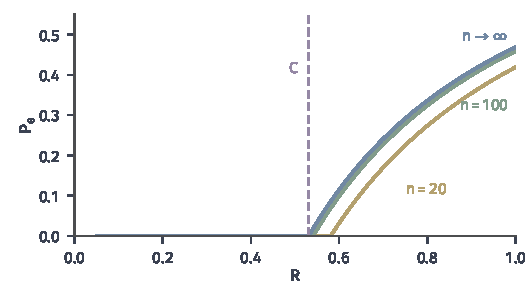
\includegraphics[width=90mm]{figures/07-probability/06-channel-coding/matplotlib/dcc-fano-bound/figure.pdf}
 \caption{翻转概率$0.1$的二元对称信道上，任何$M\geq2^{nR}$的码的平均错误概率下界$1-C/R-1/(nR)$（负值截为零），作为码率$R$的函数：黄线$n=20$，绿线$n=100$，蓝线为$n\to\infty$的极限$1-C/R$；紫色虚线为容量$C=0.531$。}
 \label{fig:dcc-fano-bound}
\end{BookInlineFigure}

证明在两个地方用到了模型假设。数据处理的第二步需要“给定码字后输出与消息无关”，有反馈时编码器的后续输入依赖此前的输出，这一步要重新论证。引理~\ref{lem:dcc-block-bound}需要无记忆。另外，下界$1-C/R$只说错误不能趋于零，并没有说错误趋于$1$。离散无记忆信道上，码率高于容量时错误概率实际上趋于$1$，这称为强逆定理；证明要控制信息密度的集中程度，而不只是它的均值，篇幅较长，可查阅~\scite{math-cover2006information}。

\subsection{最大错误概率}
\label{sec:dcc-max-error}

可达性证明控制的是平均错误概率：大多数消息很少出错，但可能有少数消息出错很多。如果消息不是均匀出现的，例如第~\ref{chap:channel-codes}章把压缩后的索引送进信道时，平均错误小并不能保证实际错误小。需要的是每条消息都可靠，即$\lambda_{\max}$小。

办法是删去坏消息。平均值为$P_{\mathrm{e}}$的一组非负数中，超过平均值两倍的不会多于一半：若超过$2P_{\mathrm{e}}$的有$k\geq1$个，则
\[
 MP_{\mathrm{e}}=\sum_{m}\lambda_m>k\cdot2P_{\mathrm{e}} ,
\]
所以$k<M/2$。这是第~\ref{chap:tail-probabilities}章Markov不等式在均匀分布上的形式。

\begin{lemma}[删去坏码字]
\label{lem:dcc-expurgation}
设$(M,n)$码的平均错误概率为$P_{\mathrm{e}}$，$M\geq2$。则可以从中保留至少$\lceil M/2\rceil$条消息，得到一个最大错误概率不超过$2P_{\mathrm{e}}$的码。
\end{lemma}

\begin{proof}
保留$\lambda_m\leq2P_{\mathrm{e}}$的消息，由上面的计数，保留的个数至少为$\lceil M/2\rceil$。码字不变；解码器把原来判给被删消息的输出块任意改判给一条保留的消息。对保留的消息$m$，判为$m$的输出块只增不减，所以它的条件错误概率不超过原来的$\lambda_m\leq2P_{\mathrm{e}}$。
\end{proof}

这一步称为\term{码字删除}（expurgation）。码率的损失是
\[
 \frac{\log_2M}{n}-\frac{\log_2\lceil M/2\rceil}{n}\leq\frac1n ,
\]
随块长趋于零。所以对$R<C$，先取$R<R'<C$，用可达性得到$M_n\geq2^{nR'}$、平均错误趋于零的码列，再删去一半消息，得到$\lceil M_n/2\rceil\geq2^{nR'-1}\geq2^{nR}$（$n$足够大时）且$\lambda_{\max}\to0$的码列。这就完成了定理~\ref{thm:dcc-coding-theorem}中关于最大错误概率的部分。反方向，最大错误不小于平均错误，逆定理对最大错误口径同样成立。两种口径给出相同的容量。

图~\ref{fig:dcc-expurgation}是一个具体的例子：随机抽取$16$个长度为$14$的二元码字（码率$\tfrac27$），在翻转概率$0.1$的二元对称信道上用最大似然解码（并列时判给编号较小的消息），对全部$2^{14}$个输出块精确求出每条消息的$\lambda_m$。平均错误概率为$0.069$，最差的消息却达到$0.253$。原因是它与另一个码字只差两位，两者似然相同的输出块按并列规则判给了编号较小的那一条，那一条的错误只有$0.040$。删去这一条消息后，剩余$15$条消息的最大错误概率为$0.127$，不超过$2P_{\mathrm{e}}=0.139$，码率变为$\log_215/14\approx0.279$。

\begin{BookInlineFigure}
 \centering
 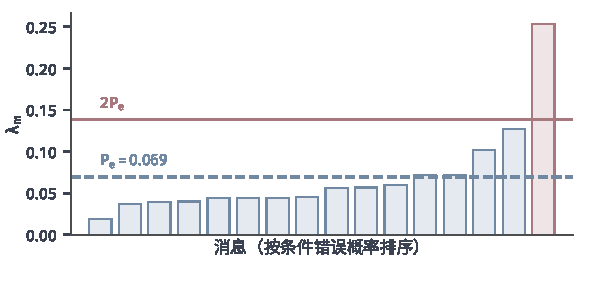
\includegraphics[width=100mm]{figures/07-probability/06-channel-coding/matplotlib/dcc-expurgation/figure.pdf}
 \caption{一个随机二元码（$16$个码字，长度$14$，随机种子$1$）在翻转概率$0.1$的二元对称信道上用最大似然解码时，各消息的条件错误概率$\lambda_m$，按大小排序，均为精确值。蓝色虚线为平均错误概率$0.069$，红线为其两倍；红色柱是被删去的消息。}
 \label{fig:dcc-expurgation}
\end{BookInlineFigure}

删除只在渐近意义下“免费”：$1/n$比特的损失随块长消失，但在有限块长下它是真实的代价。对短码，设计时直接控制每条消息的错误，比事后删除更合适。


\section{二元信道的容量}
\label{sec:dcc-binary}

翻转与擦除是二元输入上最基本的两种损坏。它们的容量各是多少？损坏的概率相同时，哪一种更伤害传输？两个信道都有一个对称性：把输入的$0$与$1$互换，同时把输出的$0$与$1$互换（擦除符号不动），转移矩阵不变。

对称性给出最优输入的候选。若$q$是最优输入分布，把它的两个分量互换得到$\tilde{q}$，由于信道在互换下不变，$I(\tilde{q})=I(q)=C$。由定理~\ref{thm:dcc-capacity-exists}，最优输入组成凸集，所以$\tfrac12q+\tfrac12\tilde{q}=(\tfrac12,\tfrac12)$也最优。于是两个信道的容量都在均匀输入处取到。下面直接算出这个值，再用上界~\eqref{eq:dcc-upper-bound}独立核验。

\subsection{二元对称信道}
\label{sec:dcc-bsc}

设翻转概率为$p\in[0,1]$。给定任一输入，输出是“翻”或“不翻”的二选一，概率为$p$与$1-p$，条件熵是二元熵$h_2(p)$，与输入分布无关：
\[
 H(Y\mid X)=\sum_xq(x)H(W_x)=h_2(p) .
\]
所以互信息只通过输出熵依赖输入分布：
\[
 I(q)=H(Y)-h_2(p)\leq1-h_2(p) ,
\]
因为$Y$只取两个值，$H(Y)\leq1$。均匀输入时，$p_q(1)=\tfrac12(1-p)+\tfrac12p=\tfrac12$，输出均匀，$H(Y)=1$，等号成立。于是
\begin{equation}
 C_{\mathrm{BSC}}(p)=1-h_2(p) .
 \label{eq:dcc-bsc-capacity}
\end{equation}

用式~\eqref{eq:dcc-upper-bound}核验：取$r=(\tfrac12,\tfrac12)$，两行到$r$的散度相同，
\[
 D_{\mathrm{KL}}(W_0\Vert r)=(1-p)\log_2\bigl(2(1-p)\bigr)+p\log_2(2p)=1-h_2(p) ,
\]
$W_1$的计算只是交换两项。所以$C\leq1-h_2(p)$，而均匀输入达到这个值。这一核验不依赖对称性论证，也说明条件~\eqref{eq:dcc-kkt}在均匀输入处成立。

$p=0.1$时，
\[
 h_2(0.1)=0.1\log_210+0.9\log_2\tfrac{10}{9}\approx0.469 ,
\]
容量约为$0.531$比特每次使用。三次重复码以码率$\tfrac13$达到$0.028$的错误；编码定理说，用足够长的码，码率可以接近$0.531$而错误仍趋于零。

\paragraph{端点}
$p=0$时信道无噪声，$C=1$。$p=\tfrac12$时输出与输入独立，无论发什么，接收端看到的都是公平硬币，$C=0$。$p=1$时每个符号都被翻转，但翻转是确定的，接收端把收到的符号全部取反就能完全恢复，$C=1-h_2(1)=1$。所以“翻转发生”与“信息损失”不是一回事：损失来自不知道哪些符号被翻转，即翻转的不可预测性。$h_2(p)$关于$p=\tfrac12$对称，翻转概率$0.9$与$0.1$的信道容量相同。

\subsection{二元擦除信道}
\label{sec:dcc-bec}

设擦除概率为$\varepsilon\in[0,1]$，输出取$0$、$\mathrm{e}$、$1$。这里换一个分解更方便：$I(X;Y)=H(X)-H(X\mid Y)$，计算接收端看到输出后对输入还剩多少不确定性。

看到$0$或$1$时，输入就是这个值，没有剩余的不确定性。看到$\mathrm{e}$时，因为擦除与输入无关，
\[
 \mathbb{P}(X=x\mid Y=\mathrm{e})=\frac{q(x)\varepsilon}{\varepsilon}=q(x) ,
\]
输入仍是原来的分布，剩余$H(X)$。$Y=\mathrm{e}$的概率是$\varepsilon$，所以$H(X\mid Y)=\varepsilon H(X)$，并且
\[
 I(q)=(1-\varepsilon)H(X)\leq1-\varepsilon .
\]
均匀输入使$H(X)=1$，等号成立：
\begin{equation}
 C_{\mathrm{BEC}}(\varepsilon)=1-\varepsilon .
 \label{eq:dcc-bec-capacity}
\end{equation}
这个结果有直接的读法：平均有比例$1-\varepsilon$的符号原样到达，每个携带一比特，被擦除的符号什么也不携带。

核验上界：均匀输入的输出分布是
\[
 r=\Bigl(\frac{1-\varepsilon}2,\ \varepsilon,\ \frac{1-\varepsilon}2\Bigr) ,
\]
第一行到它的散度为
\[
 D_{\mathrm{KL}}(W_0\Vert r)=(1-\varepsilon)\log_2\frac{1-\varepsilon}{(1-\varepsilon)/2}+\varepsilon\log_2\frac{\varepsilon}{\varepsilon}=1-\varepsilon ,
\]
第二行相同（$0<\varepsilon<1$；$\varepsilon=1$时两行都是集中在$\mathrm{e}$上的分布，散度为$0$）。由式~\eqref{eq:dcc-upper-bound}，$C\leq1-\varepsilon$。端点$\varepsilon=0$给出无噪声信道的$1$，$\varepsilon=1$时什么也收不到，容量为$0$。

\paragraph{已知错误位置的价值}
比较损坏概率相同的两个信道。图~\ref{fig:dcc-flip-vs-erasure}把同一个输入块分别送进两个信道，在同样两个位置发生损坏。擦除信道的接收端看到$\mathrm{e}$，确切知道哪里缺了信息，其余位置完全可信；对称信道的接收端看到的是普通的$0$和$1$，不知道哪两位是错的，每一位都只能部分相信。

\begin{BookInlineFigure}
 \centering
 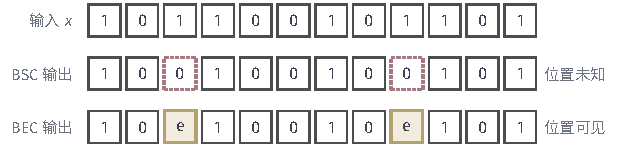
\includegraphics[width=104.5mm]{figures/07-probability/06-channel-coding/tikz/dcc-flip-vs-erasure/figure.pdf}
 \caption{同一个$12$位输入块在第$3$、$9$位受到损坏。二元对称信道把这两位翻转，结果看起来与其他位无异，红色虚线框只是标给读者看的；二元擦除信道把这两位变成可见的擦除符号$\mathrm{e}$（黄色）。}
 \label{fig:dcc-flip-vs-erasure}
\end{BookInlineFigure}

图~\ref{fig:dcc-capacity-curves}比较两条容量曲线。损坏概率都是$0.1$时，擦除信道的容量是$0.9$，对称信道只有$0.531$。差值$h_2(p)-p$可以理解为找出错误位置的代价：在$n$个符号中指出约$np$个翻转位置，需要约$nh_2(p)$比特的描述，而擦除信道把这些位置免费告诉了接收端，只损失被擦掉的$np$比特本身。对$0<p<\tfrac12$总有$h_2(p)>p$，所以未知的翻转总比可见的擦除更伤害传输。

\begin{BookInlineFigure}
 \centering
 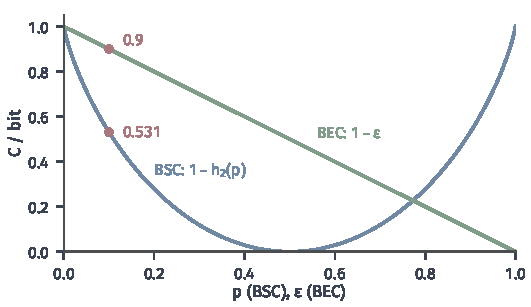
\includegraphics[width=90mm]{figures/07-probability/06-channel-coding/matplotlib/dcc-capacity-curves/figure.pdf}
 \caption{二元对称信道的容量$1-h_2(p)$（蓝）与二元擦除信道的容量$1-\varepsilon$（绿），横轴为翻转概率或擦除概率。红点标出损坏概率$0.1$时的两个容量$0.531$与$0.9$。蓝线关于$p=\tfrac12$对称：确定的翻转不损失信息。}
 \label{fig:dcc-capacity-curves}
\end{BookInlineFigure}

\paragraph{对称性的作用}
两个信道的均匀输入最优，依赖的是交换$0$与$1$的对称性，不是二元输入本身。第~\ref{sec:dcc-capacity-formula}节的Z信道同样是二元输入，却没有这种对称性：输入$1$会出错而输入$0$不会，最优输入是$q=0.4$，均匀输入少得约$0.011$比特。对一般的转移矩阵，最优输入要从条件~\eqref{eq:dcc-kkt}解出，通常没有闭式，这就需要第~\ref{sec:dcc-numerical}节的数值方法。


\section{输入成本约束}
\label{sec:dcc-costs}

实际发送时，不同符号的代价往往不同。在Z信道中，可以把输入$1$想成发出一个脉冲、输入$0$想成保持静默：脉冲消耗能量，静默不消耗。若能量有限，就不能随意多发$1$。预算会怎样限制传输速率？

给每个输入符号指定一个有限的非负成本$c(x)$，记最小成本$c_{\min}=\min_xc(x)$。设定预算$\Gamma\geq c_{\min}$，要求每一条码字都满足
\begin{equation}
 \sum_{i=1}^{n}c\bigl(x_i(m)\bigr)\leq n\Gamma,\qquad m=1,\dots,M .
 \label{eq:dcc-codeword-budget}
\end{equation}
这里的平均是沿同一条码字的$n$次使用求平均：每次传输一条消息都要守住预算。它不允许一部分消息超支、另一部分消息节省来互相抵消。在预算$\Gamma$下的可达速率按定义~\ref{def:dcc-achievable}定义，只是要求码列中的每个码都满足式~\eqref{eq:dcc-codeword-budget}。本节的例子是Z信道，取$c(0)=0$、$c(1)=1$，于是预算$\Gamma=0.25$意味着每条码字中$1$的个数不超过$n/4$。

\subsection{成本约束下的容量}
\label{sec:dcc-cost-capacity}

无约束时容量是互信息在整个单纯形上的最大值。有预算时，自然的猜测是只在“平均成本不超过预算”的输入分布上取最大值。

\begin{definition}[容量—成本函数]
\label{def:dcc-capacity-cost}
对$\Gamma\geq c_{\min}$，定义
\begin{equation}
 C(\Gamma)=\max\Bigl\{I(q):q\in\Delta_{\mathcal{X}},\ \sum_{x}q(x)c(x)\leq\Gamma\Bigr\} ,
 \label{eq:dcc-capacity-cost}
\end{equation}
称为\term{容量—成本函数}（capacity-cost function）。
\end{definition}

可行集合非空：集中在某个最小成本符号上的分布满足约束。下面的定理列出$C(\Gamma)$的基本性质。

\begin{theorem}[容量—成本函数的性质]
\label{thm:dcc-capacity-cost}
在$[c_{\min},\infty)$上，式~\eqref{eq:dcc-capacity-cost}的最大值存在；$C(\Gamma)$单调不减、是凹函数，在$(c_{\min},\infty)$上连续，并且$C(\Gamma)\leq C$；若某个无约束最优输入的平均成本为$\Gamma^{*}$，则$\Gamma\geq\Gamma^{*}$时$C(\Gamma)=C$。
\end{theorem}

\begin{proof}
可行集合是单纯形与一个闭半空间的交，非空且有界闭，$I$连续，所以最大值存在。预算增大时可行集合变大，最大值不减；它总是整个单纯形的子集，所以$C(\Gamma)\leq C$；$\Gamma\geq\Gamma^{*}$时可行集合包含无约束最优输入，所以取到$C$。

凹性。取预算$\Gamma_1,\Gamma_2$及相应的最优输入$q_1,q_2$，$\theta\in[0,1]$。混合$q_\theta=\theta q_1+(1-\theta)q_2$的平均成本是$\theta\Gamma_1+(1-\theta)\Gamma_2$以下，所以在该预算下可行；由$I$的凹性，
\[
 C\bigl(\theta\Gamma_1+(1-\theta)\Gamma_2\bigr)\geq I(q_\theta)\geq\theta C(\Gamma_1)+(1-\theta)C(\Gamma_2) .
\]
有限的凹函数在开区间内部连续，所以$C$在$(c_{\min},\infty)$上连续。
\end{proof}

在端点$c_{\min}$处，$C$未必右连续。凹性说明预算越多，每多一单位预算带来的容量增量越小，直到达到$\Gamma^{*}$后增量为零。

\paragraph{Z信道的例子}
平均成本是$\sum_xq(x)c(x)=q$，约束就是$q\leq\Gamma$。由第~\ref{sec:dcc-capacity-formula}节，$I(q)=h_2(q/2)-q$在$[0,0.4]$上递增、在$0.4$处达到最大值。所以
\[
 C(\Gamma)=h_2\Bigl(\frac\Gamma2\Bigr)-\Gamma\quad(0\leq\Gamma\leq0.4),\qquad C(\Gamma)=\log_2\frac54\quad(\Gamma\geq0.4) .
\]
预算$\Gamma=0.25$时，最优输入为$q=0.25$，
\[
 C(0.25)=h_2(0.125)-0.25\approx0.5436-0.25=0.2936 ,
\]
比无约束容量$0.3219$少约$0.028$比特。图~\ref{fig:dcc-cost-capacity}(a)画出可行的输入范围，(b)画出整条$C(\Gamma)$曲线：它先凹地上升，在$\Gamma=0.4$之后变平。

\begin{BookInlineFigure}
 \centering
 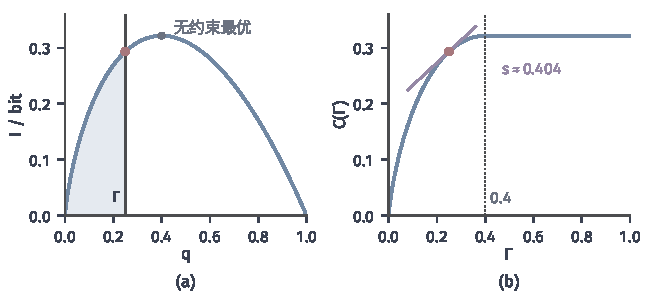
\includegraphics[width=110mm]{figures/07-probability/06-channel-coding/matplotlib/dcc-cost-capacity/figure.pdf}
 \caption{Z信道在成本$c(0)=0$、$c(1)=1$下的容量—成本函数。(a) 互信息$I(q)=h_2(q/2)-q$，浅蓝区域是预算$\Gamma=0.25$允许的输入$q\leq\Gamma$，红点为约束下的最优点，灰点为无约束最优点$q=0.4$；(b) $C(\Gamma)$，紫线是$\Gamma=0.25$处的切线，斜率$s\approx0.404$比特每单位成本，点线标出$\Gamma=0.4$。}
 \label{fig:dcc-cost-capacity}
\end{BookInlineFigure}

\paragraph{Lagrange乘子：预算的边际价值}
图~\ref{fig:dcc-cost-capacity}(b)中切线的斜率回答“再多给一单位预算，容量能增加多少”。把约束用乘子$s\geq0$并入目标，考虑
\begin{equation}
 \max_{q\in\Delta_{\mathcal{X}}}\Bigl[I(q)-s\sum_xq(x)c(x)\Bigr]+s\Gamma .
 \label{eq:dcc-lagrangian}
\end{equation}
对每个$s\geq0$与每个可行的$q$，被减去的$s(\sum_xq(x)c(x)-\Gamma)$非正，所以$I(q)$不超过式~\eqref{eq:dcc-lagrangian}；对可行的$q$取最大值，得到
\begin{equation}
 C(\Gamma)\leq\max_{q}\Bigl[I(q)-s\sum_xq(x)c(x)\Bigr]+s\Gamma\qquad\text{对每个}\ s\geq0 .
 \label{eq:dcc-weak-duality}
\end{equation}
这是弱对偶。$\Gamma>c_{\min}$时，集中在最小成本符号上的分布严格满足预算，目标是凹函数，约束是线性的，于是强对偶成立：式~\eqref{eq:dcc-weak-duality}右边对$s$的最小值等于$C(\Gamma)$，达到最小值的$s$是$C$在$\Gamma$处的切线斜率（$C$在该点可微时）。凸优化对偶的一般理论可参考\BookChapterRef{chap:duality}{卷五第18章“对偶问题”}。

固定$s$后，式~\eqref{eq:dcc-lagrangian}中的最大化与定理~\ref{thm:dcc-kkt}的问题相同，只是线性项多了$-s\sum_xq(x)c(x)$。在定理~\ref{thm:dcc-kkt}必要性的求导中，这一项沿$q_t=(1-t)q^{*}+t\delta_{x'}$的右导数是$-s\bigl(c(x')-\sum_xq^{*}(x)c(x)\bigr)$，充分性部分的上界也照样成立。所以最优条件变为：存在常数$c'$，使
\begin{equation}
 \begin{aligned}
 D_{\mathrm{KL}}(W_x\Vert p^{*})-s\,c(x)&=c'\quad\text{若}\ q^{*}(x)>0 ,\\
 D_{\mathrm{KL}}(W_x\Vert p^{*})-s\,c(x)&\leq c'\quad\text{若}\ q^{*}(x)=0 .
 \end{aligned}
 \label{eq:dcc-kkt-cost}
\end{equation}
读法是：每个输入的信息贡献扣去它按“影子价格”$s$折算的成本后，被使用的输入应当一样划算。

在Z信道$\Gamma=0.25$处核验。斜率为
\[
 s=I'(0.25)=\frac12\log_2\frac{2-0.25}{0.25}-1=\frac12\log_27-1\approx0.4037 .
\]
输出分布$p^{*}=(\tfrac78,\tfrac18)$，两行的散度为
\[
 \begin{aligned}
 D_{\mathrm{KL}}(W_0\Vert p^{*})&=\log_2\frac87\approx0.1926 ,\\
 D_{\mathrm{KL}}(W_1\Vert p^{*})&=\frac12\log_2\frac47+\frac12\log_24=\frac12\log_2\frac{16}7\approx0.5963 .
 \end{aligned}
\]
扣去成本后，$0.1926-0=0.1926$，$0.5963-0.4037=0.1926$，两者相等；并且$C(\Gamma)-s\Gamma=0.2936-0.1009=0.1927$，与舍入误差内一致。精确地，
\[
 \frac12\log_2\frac{16}7-\Bigl(\frac12\log_27-1\Bigr)=3-\log_27=\log_2\frac87 .
\]

\paragraph{期望约束与逐条预算}
式~\eqref{eq:dcc-capacity-cost}约束的是输入分布的期望成本，它是对单个随机符号的设计要求；式~\eqref{eq:dcc-codeword-budget}约束的是每一条具体码字的成本总和。按期望成本恰为$\Gamma$的分布独立抽取码字，大约一半码字会超出预算。两者之间的联系需要论证，这是下一小节的内容。

\subsection{满足预算的编码}
\label{sec:dcc-cost-coding}

下面的定理说明，在逐条预算下，$C(\Gamma)$正是可靠传输的速率极限。

\begin{theorem}[成本约束下的编码定理]
\label{thm:dcc-cost-coding}
设$\Gamma>c_{\min}$。在每条码字满足式~\eqref{eq:dcc-codeword-budget}的要求下，每个$R<C(\Gamma)$都可达，并且可以要求最大错误概率趋于零；每个$R>C(\Gamma)$都不可达。
\end{theorem}

\begin{proof}
可达性。设$R<C(\Gamma)$。由定理~\ref{thm:dcc-capacity-cost}，$C$在$\Gamma$处连续，可以取$\Gamma'\in(c_{\min},\Gamma)$使$C(\Gamma')>R$。取$q'$使$\sum_xq'(x)c(x)\leq\Gamma'$且$I(q')=C(\Gamma')$。这一步为预算留出了余量$\Gamma-\Gamma'>0$。

按$q'$抽取随机码本，用联合典型解码。定理~\ref{thm:dcc-achievability}的证明对任何满足$I(q)>R$的输入分布都成立，所以存在$\delta_n\to0$，使每条消息的期望错误$\mathbb{E}[\lambda_m]\leq\delta_n$。另一方面，记$B_m$为第$m$条码字超出预算的事件。码字的平均成本$\frac1n\sum_ic(\mathsf{X}_i(m))$是$n$个独立同分布、取值有界的变量的平均，均值不超过$\Gamma'<\Gamma$，由弱大数律，
\[
 \beta_n=\mathbb{P}(B_m)\leq\mathbb{P}\Bigl(\frac1n\sum_{i=1}^{n}c(\mathsf{X}_i(m))-\Gamma'>\Gamma-\Gamma'\Bigr)\to0 .
\]
于是随机码本满足
\[
 \mathbb{E}\Bigl[P_{\mathrm{e}}+\frac1M\sum_{m=1}^{M}\mathbf{1}_{B_m}\Bigr]\leq\delta_n+\beta_n=:\eta_n ,
\]
存在一个具体码本，其平均错误概率与超支码字的比例之和不超过$\eta_n$。

删去两类消息：条件错误概率超过$4\eta_n$的消息，按第~\ref{sec:dcc-max-error}小节的计数少于$M/4$条；超支的消息，至多$\eta_nM$条，$n$足够大使$\eta_n\leq\tfrac14$时不超过$M/4$条。保留的消息至少有$M/2$条，每条码字都守住预算，最大错误概率不超过$4\eta_n$，码率损失不超过$1/n$。与引理~\ref{lem:dcc-expurgation}后的论证一样，先用$R<R'<C(\Gamma)$构造码列再删除，就得到码率不低于$R$的码列。

逆定理。设一列满足逐条预算的码有$M\geq2^{nR}$且$P_{\mathrm{e}}\to0$。消息均匀，记第$i$个输入符号$X_i$的分布为$q_i$，期望成本$\Gamma_i=\mathbb{E}[c(X_i)]$。逆定理证明中的Fano与数据处理步骤不变，引理~\ref{lem:dcc-block-bound}的第一个不等式给出
\[
 \log_2M\leq1+P_{\mathrm{e}}\log_2M+\sum_{i=1}^{n}I(X_i;Y_i)\leq1+P_{\mathrm{e}}\log_2M+\sum_{i=1}^{n}C(\Gamma_i) .
\]
由$C$的凹性（Jensen不等式）与单调性，
\[
 \frac1n\sum_{i=1}^{n}C(\Gamma_i)\leq C\Bigl(\frac1n\sum_{i=1}^{n}\Gamma_i\Bigr)\leq C(\Gamma) ,
\]
最后一步因为
\[
 \frac1n\sum_{i=1}^{n}\Gamma_i=\mathbb{E}\Bigl[\frac1n\sum_{i=1}^{n}c(X_i)\Bigr]\leq\Gamma :
\]
每条码字的平均成本都不超过$\Gamma$，对消息平均后也不超过。于是$P_{\mathrm{e}}\geq1-(nC(\Gamma)+1)/\log_2M$，与定理~\ref{thm:dcc-converse}同理，$R>C(\Gamma)$不可达。
\end{proof}

可达性证明中的两个余量各有作用。码率余量$C(\Gamma')-R>0$控制解码错误，与无约束时相同；预算余量$\Gamma-\Gamma'>0$让大数律把码字成本压在预算以内。若直接用期望成本恰为$\Gamma$的分布，超支的码字比例不趋于零，删除会损失一个固定比例的消息。图~\ref{fig:dcc-codeword-cost}画出Z信道上$q'=0.22$、$\Gamma=0.25$时单条随机码字的平均成本分布：$n=50$时超支的概率约为$0.296$，$n=400$时降到约$0.067$，并继续趋于零。所用输入的互信息为$C(0.22)=h_2(0.11)-0.22\approx0.280$，略低于$C(0.25)=0.294$，这是为预算余量付出的码率。

\begin{BookInlineFigure}
 \centering
 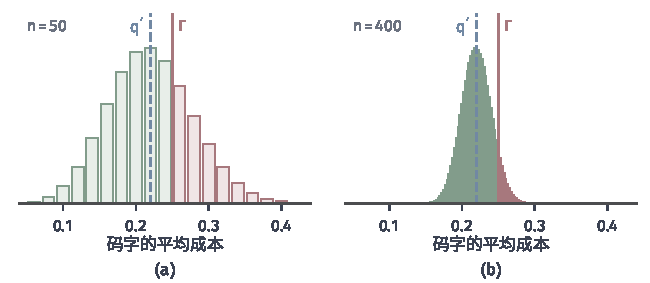
\includegraphics[width=110mm]{figures/07-probability/06-channel-coding/matplotlib/dcc-codeword-cost/figure.pdf}
 \caption{Z信道、成本$c(1)=1$，码字符号独立地以概率$q'=0.22$取$1$时，单条码字的平均成本$K/n$（$K\sim\mathrm{Bin}(n,0.22)$）的精确分布。蓝色虚线为$q'$，红线为预算$\Gamma=0.25$，红色柱为超出预算的码字。(a) $n=50$；(b) $n=400$。}
 \label{fig:dcc-codeword-cost}
\end{BookInlineFigure}

逆定理只用到了“对消息平均的成本不超过$\Gamma$”。所以即使放宽要求，只限制各码字成本的平均值，容量也不会超过$C(\Gamma)$；而可达性给出的码满足更严格的逐条预算。两种口径给出同一个容量。

\paragraph{预算等于最小成本}
$\Gamma=c_{\min}$时，余量论证无法进行，因为不存在$\Gamma'<\Gamma$。但此时约束本身变得简单：每个$c(x_i)\geq c_{\min}$，总和不超过$nc_{\min}$只能让每一项都等于$c_{\min}$。所以码字只能使用集合$\mathcal{X}_0=\{x:c(x)=c_{\min}\}$中的符号，成本约束自动满足。这相当于把输入字母表缩小为$\mathcal{X}_0$、转移矩阵只保留相应的行，对这个新信道应用无约束的定理~\ref{thm:dcc-coding-theorem}，容量为$\max\{I(q):q\ \text{支撑在}\ \mathcal{X}_0\ \text{上}\}$。这恰好等于$C(c_{\min})$，因为平均成本等于$c_{\min}$的分布正是支撑在$\mathcal{X}_0$上的分布。在Z信道中$\mathcal{X}_0=\{0\}$，只能发送$0$，容量为零。


\section{容量的数值计算}
\label{sec:dcc-numerical}

对称信道和Z信道的容量都能手算，一般的转移矩阵却不行：条件~\eqref{eq:dcc-kkt}是关于$q$的非线性方程组，还带着“哪些输入概率为零”的组合选择。互信息是单纯形上的凹函数，原则上任何凸优化方法都能求最大值；但这个问题有特殊结构，可以得到每步都有闭式、自动留在单纯形内、并且随时给出容量上下界的迭代。它称为\term{Blahut–Arimoto算法}（Blahut–Arimoto algorithm）。

\paragraph{主要思想}
出发点是式~\eqref{eq:dcc-mi-divergence}：互信息是各输入的信息贡献$D_{\mathrm{KL}}(W_x\Vert p_q)$按$q$的平均。若某个输入的贡献高于平均，就应当多用它。Blahut–Arimoto算法把这个直觉做成乘性的重新加权，下面从一个双变量的目标推出它。

引入一个“反向”的条件分布$r(x\mid y)$：对每个$y$，$r(\cdot\mid y)$是$\mathcal{X}$上的概率分布，它表示接收端看到$y$后对输入的猜测。定义
\[
 J(q,r)=\sum_{x,y}q(x)W(y\mid x)\log_2\frac{r(x\mid y)}{q(x)} .
\]
固定$q$时，最好的猜测是真实的后验$r_q(x\mid y)=q(x)W(y\mid x)/p_q(y)$。因为$r_q(x\mid y)/q(x)=W(y\mid x)/p_q(y)$，所以$J(q,r_q)=I(q)$；而对任意$r$，
\[
 \begin{aligned}
 I(q)-J(q,r)&=\sum_{x,y}q(x)W(y\mid x)\log_2\frac{r_q(x\mid y)}{r(x\mid y)}\\
 &=\sum_yp_q(y)\,D_{\mathrm{KL}}\bigl(r_q(\cdot\mid y)\Vert r(\cdot\mid y)\bigr)\geq0 .
 \end{aligned}
\]
于是$I(q)=\max_rJ(q,r)$，容量可以写成两个变量的联合最大值
\begin{equation}
 C=\max_{q}\max_{r}J(q,r) .
 \label{eq:dcc-ba-double-max}
\end{equation}

反过来固定$r$，对$q$最大化。记$a(x)=\sum_yW(y\mid x)\log_2r(x\mid y)$，目标是$\sum_xq(x)\bigl(a(x)-\log_2q(x)\bigr)$。令$\tilde{q}(x)=2^{a(x)}/Z$，$Z=\sum_x2^{a(x)}$，则
\[
 \sum_xq(x)\bigl(a(x)-\log_2q(x)\bigr)=\log_2Z-D_{\mathrm{KL}}(q\Vert\tilde{q}) ,
\]
所以最大值点是$q=\tilde{q}$，最大值是$\log_2Z$。

两步交替进行：由$q_t$取后验$r_{q_t}$，再由它算出新的$q_{t+1}$。代入后验，
\[
 a(x)=\log_2q_t(x)+\sum_{y}W(y\mid x)\log_2\frac{W(y\mid x)}{p_{q_t}(y)} ,
\]
后一项正是第$x$行的散度。记
\[
 p_t=p_{q_t},\qquad D_t(x)=D_{\mathrm{KL}}\bigl(W_x\Vert p_t\bigr) ,
\]
得到更新公式
\begin{equation}
 q_{t+1}(x)=\frac{q_t(x)\,2^{D_t(x)}}{\sum_{x'}q_t(x')\,2^{D_t(x')}} .
 \label{eq:dcc-ba-update}
\end{equation}
贡献$D_t(x)$大的输入按指数放大，小的相对缩小，与开头的直觉一致。不动点处，凡是$q(x)>0$的输入，$2^{D(x)}$必须等于归一化常数，即散度相等，这正是条件~\eqref{eq:dcc-kkt}。

每一轮还能顺带得到容量的上下界。下界：$\log_2\sum_xq_t(x)2^{D_t(x)}$是$J(q_{t+1},r_{q_t})$，不超过$I(q_{t+1})$，更不超过$C$。上界：在式~\eqref{eq:dcc-upper-bound}中取$r=p_t$。于是
\begin{equation}
 L_t=\log_2\sum_xq_t(x)\,2^{D_t(x)}\ \leq\ C\ \leq\ U_t=\max_xD_t(x) .
 \label{eq:dcc-ba-bounds}
\end{equation}
两个界都是严格成立的不等式，不是估计值；$U_t-L_t$就是当前对容量的误差保证。交替对两个变量分别取最大的做法，是卷五分块坐标方法的一个特例，可参考\BookChapterRef{chap:block-optimization}{卷五第12章“分块优化”}。第~\ref{chap:rate-distortion}章计算率失真函数时用的是同一结构，只是那里最小化，并带有失真的指数权重。

\paragraph{计算过程}
下面以Z信道为例走一遍，转移矩阵的两行是$W_0=(1,0)$与$W_1=(\tfrac12,\tfrac12)$。

\needspace{6\baselineskip}
\paragraph{变量}
\begin{itemize}
 \item $q_t$：长度为$\lvert\mathcal{X}\rvert$的概率向量，第$t$轮的输入分布；
 \item $p_t$：长度为$\lvert\mathcal{Y}\rvert$的概率向量，$p_t=q_t\bm{W}$；
 \item $D_t$：长度为$\lvert\mathcal{X}\rvert$的向量，$D_t(x)=D_{\mathrm{KL}}(W_x\Vert p_t)$；
 \item $L_t,U_t$：容量的下界与上界；$\tau>0$：要求的精度。
\end{itemize}

\paragraph{初始化}
取支撑为整个$\mathcal{X}$的初始分布，通常取均匀分布$q_0(x)=1/\lvert\mathcal{X}\rvert$。例中$q_0=(\tfrac12,\tfrac12)$，$\tau=0.01$。

\needspace{6\baselineskip}
\paragraph{每轮更新}
对$t=0,1,2,\dots$依次执行：
\begin{enumerate}
 \item 输出分布：$p_t=q_t\bm{W}$。例中第$0$轮，
 \[
  p_0=\tfrac12(1,0)+\tfrac12(\tfrac12,\tfrac12)=(\tfrac34,\tfrac14) .
 \]

 \item 各行散度：按$D_t(x)=D_{\mathrm{KL}}(W_x\Vert p_t)$计算，$W(y\mid x)=0$的项记为零。例中
 \[
  \begin{aligned}
  D_0(0)&=\log_2\frac43\approx0.4150 ,\\
  D_0(1)&=\frac12\log_2\frac{1/2}{3/4}+\frac12\log_2\frac{1/2}{1/4}=\frac12\log_2\frac43\approx0.2075 .
  \end{aligned}
 \]

 \item 上下界：由式~\eqref{eq:dcc-ba-bounds}计算。例中$2^{D_0(0)}=\tfrac43$，$2^{D_0(1)}=\tfrac{2}{\sqrt3}\approx1.1547$，
 \[
  L_0=\log_2\Bigl(\tfrac12\cdot\tfrac43+\tfrac12\cdot1.1547\Bigr)=\log_21.2440\approx0.3150 ,
 \]
 \[
  U_0=\max\{0.4150,\ 0.2075\}=0.4150 .
 \]
 若$U_t-L_t\leq\tau$，停止。例中差距为$0.1000$，继续。

 \item 重新加权：由式~\eqref{eq:dcc-ba-update}，
 \[
  q_1=\frac{(0.6667,\ 0.5774)}{1.2440}=(0.5359,\ 0.4641) .
 \]
 精确值是$q_1(1)=2\sqrt3-3$。输入$1$的贡献低于平均，它的概率下降了。
\end{enumerate}

例中第$1$轮的四步依次得到
\[
 p_1=(0.7679,\ 0.2321),\qquad D_1=(0.3809,\ 0.2442) ,
\]
\[
 L_1=\log_2(0.5359\times1.3021+0.4641\times1.1844)\approx0.3191,\qquad U_1\approx0.3809 ,
\]
差距为$0.0618$，更新得$q_2=(0.5594,0.4406)$。各轮结果如下表。

\begin{BookInlineTable}
 \centering
 \caption{Z信道上Blahut–Arimoto迭代的各轮数值，$q_0=(\tfrac12,\tfrac12)$，容量真值为$\log_2(5/4)\approx0.32193$。}
 \label{tab:dcc-ba-rounds}
 \begin{tabular}{cccccc}
  \toprule
  $t$ & $q_t(1)$ & $D_t(0)$ & $D_t(1)$ & $L_t$ & $U_t$ \\
  \midrule
  $0$ & $0.50000$ & $0.41504$ & $0.20752$ & $0.31501$ & $0.41504$ \\
  $1$ & $0.46410$ & $0.38092$ & $0.24420$ & $0.31907$ & $0.38092$ \\
  $2$ & $0.44063$ & $0.35904$ & $0.27070$ & $0.32078$ & $0.35904$ \\
  $3$ & $0.42560$ & $0.34520$ & $0.28882$ & $0.32147$ & $0.34520$ \\
  $4$ & $0.41607$ & $0.33649$ & $0.30079$ & $0.32175$ & $0.33649$ \\
  $5$ & $0.41007$ & $0.33104$ & $0.30854$ & $0.32186$ & $0.33104$ \\
  \bottomrule
 \end{tabular}
\end{BookInlineTable}

第$5$轮差距$U_5-L_5=0.0092\leq0.01$，停止。最终得到容量的保证区间与近似最优输入
\[
 0.32186\leq C\leq0.33104,\qquad q_5\approx(0.590,\ 0.410) .
\]
真值$0.32193$确实在区间内，最优输入是$(0.6,0.4)$。图~\ref{fig:dcc-ba-z}画出更多轮次：$q_t(1)$单调地趋向$0.4$；下界几乎一开始就贴近容量，上界下降较慢，差距主要由上界决定。

\begin{BookInlineFigure}
 \centering
 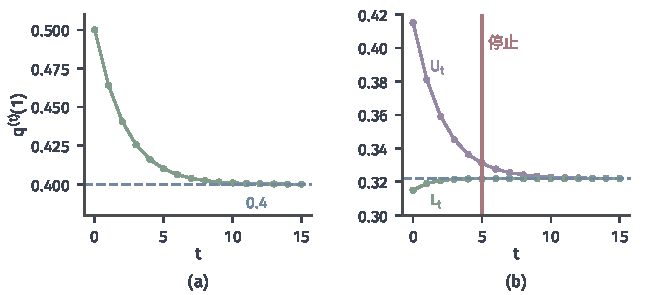
\includegraphics[width=110mm]{figures/07-probability/06-channel-coding/matplotlib/dcc-ba-z/figure.pdf}
 \caption{Z信道上从$q_0=(\tfrac12,\tfrac12)$出发的Blahut–Arimoto迭代。(a) 绿点为$q_t(1)$，蓝色虚线为最优值$0.4$；(b) 紫线为上界$U_t$，绿线为下界$L_t$，蓝色虚线为容量$\log_2(5/4)$，红线标出第一次满足$U_t-L_t\leq0.01$的轮次$t=5$。}
 \label{fig:dcc-ba-z}
\end{BookInlineFigure}

\paragraph{收敛性}
下界的收敛可以完整证明，并且给出速度。

\begin{theorem}[Blahut–Arimoto迭代的收敛]
\label{thm:dcc-ba-convergence}
设$q_0$的支撑是整个$\mathcal{X}$，$q^{*}$是任一最优输入分布。则$I(q_t)$与$L_t$都单调不减，并且
\begin{equation}
 C-L_T\leq\frac{D_{\mathrm{KL}}(q^{*}\Vert q_0)}{T+1},\qquad T=0,1,2,\dots .
 \label{eq:dcc-ba-rate}
\end{equation}
$q_0$均匀时右边不超过$\log_2\lvert\mathcal{X}\rvert/(T+1)$。
\end{theorem}

\begin{proof}
单调性。记$r_t=r_{q_t}$。由$J$对两个变量分别取最大的性质，
\[
 \begin{aligned}
 I(q_t)=J(q_t,r_t)&\leq J(q_{t+1},r_t)=L_t\\
 &\leq J(q_{t+1},r_{t+1})=I(q_{t+1})\leq J(q_{t+2},r_{t+1})=L_{t+1} .
 \end{aligned}
\]

速度。更新公式~\eqref{eq:dcc-ba-update}的对数形式是$\log_2\frac{q_{t+1}(x)}{q_t(x)}=D_t(x)-L_t$；$q_0$处处为正，每步乘以正数，所以$q_t$处处为正。按$q^{*}$求平均，
\[
 \sum_xq^{*}(x)\log_2\frac{q_{t+1}(x)}{q_t(x)}=\sum_xq^{*}(x)D_t(x)-L_t .
\]
定理~\ref{thm:dcc-kkt}证明中的恒等式（取$q=q^{*}$、$r=p_t$）给出
\[
 \sum_xq^{*}(x)D_t(x)=C+D_{\mathrm{KL}}(p^{*}\Vert p_t)\geq C ,
\]
所以右边不小于$C-L_t$。对$t=0,\dots,T$求和，左边逐项相消，
\[
 \begin{aligned}
 D_{\mathrm{KL}}(q^{*}\Vert q_0)-D_{\mathrm{KL}}(q^{*}\Vert q_{T+1})&=\sum_{t=0}^{T}\sum_xq^{*}(x)\log_2\frac{q_{t+1}(x)}{q_t(x)}\\
 &\geq\sum_{t=0}^{T}(C-L_t)\geq(T+1)(C-L_T) ,
 \end{aligned}
\]
最后一步用了$L_t$单调不减。$D_{\mathrm{KL}}(q^{*}\Vert q_{T+1})\geq0$，移项即得式~\eqref{eq:dcc-ba-rate}。均匀初始时
\[
 D_{\mathrm{KL}}(q^{*}\Vert q_0)=\log_2\lvert\mathcal{X}\rvert-H(q^{*})\leq\log_2\lvert\mathcal{X}\rvert .
\]
\end{proof}

上界$U_t$同样收敛到$C$，因为$p_t$收敛到唯一的最优输出分布；这一部分的证明更长，可查阅~\scite{math-cover2006information}。实践中不需要它的速度：只要算出$U_t$与$L_t$，区间$[L_t,U_t]$本身就是可验证的结论。

\paragraph{初始支撑与零概率输入}
证明中“$q_0$处处为正”不可省略。若$q_0(x)=0$，乘性更新使$q_t(x)$永远为零，迭代实际是在去掉输入$x$的信道上进行；若$x$是有用的输入，迭代会收敛到一个偏小的值。这时上界会暴露问题：$U_t$对全部输入取最大值，包括概率为零的输入，于是差距$U_t-L_t$不会趋于零。同样的原因，初始支撑完整时$p_t(y)>0$对一切可能出现的输出成立，散度不会出现除以零。

反过来，最优输入可能给某些符号零概率，迭代却只能让它们的概率趋于零而不能到达零。考虑三输入二输出的信道，三行为$(1,0)$、$(0,1)$、$(\tfrac12,\tfrac12)$：前两个输入无噪声，第三个输入的输出与输入无关。容量为$1$比特，最优输入是$(\tfrac12,\tfrac12,0)$。从均匀分布出发，由对称性$p_t=(\tfrac12,\tfrac12)$始终不变，散度始终为$(1,1,0)$，每轮第三个分量相对其余两个缩小一半：
\[
 q_t(2)=\frac{1}{2^{t+1}+1}:\qquad \tfrac13,\ \tfrac15,\ \tfrac19,\ \tfrac1{17},\ \dots
\]
上界从第$0$轮起就等于$1$，下界$L_t=\log_2(2-q_t(2))$的差距按几何速度缩小，远快于式~\eqref{eq:dcc-ba-rate}保证的$\log_23/(t+1)$。图~\ref{fig:dcc-ba-support}画出这两点。

\begin{BookInlineFigure}
 \centering
 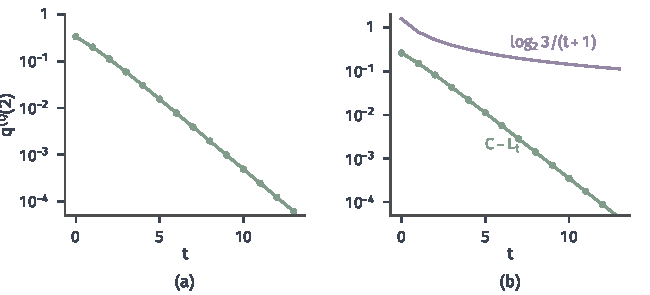
\includegraphics[width=110mm]{figures/07-probability/06-channel-coding/matplotlib/dcc-ba-support/figure.pdf}
 \caption{三行分别为$(1,0)$、$(0,1)$、$(\tfrac12,\tfrac12)$的信道上，从均匀分布出发的Blahut–Arimoto迭代，纵轴均为对数坐标。(a) 无用输入的概率$q_t(2)=1/(2^{t+1}+1)$按几何速度减小，但始终为正；(b) 绿线为下界的差距$C-L_t$，紫线为定理~\ref{thm:dcc-ba-convergence}的保证$\log_23/(t+1)$；上界$U_t$从第$0$轮起就等于$C=1$。}
 \label{fig:dcc-ba-support}
\end{BookInlineFigure}

这个例子说明两件事。第一，概率很小不等于应当为零，不能仅凭$q_t(x)$小就把输入删掉；需要删减时，应先用上下界确认删去后容量不变。第二，迭代变化小也不是停止的依据。Z信道第$7$轮以后$q_t$每轮只变化约$0.002$，差距仍有$0.004$；在收敛更慢的信道上，变化可以极小而离最优仍远。应当用的是$U_t-L_t$。

\paragraph{计算量}
每轮需要算$p_t=q_t\bm{W}$与全部散度，各需要$O(\lvert\mathcal{X}\rvert\lvert\mathcal{Y}\rvert)$次运算，更新与求界只需$O(\lvert\mathcal{X}\rvert)$。由式~\eqref{eq:dcc-ba-rate}，下界达到精度$\tau$至多需要约$\log_2\lvert\mathcal{X}\rvert/\tau$轮；实际中常快得多。

\paragraph{带成本约束的迭代}
对第~\ref{sec:dcc-costs}节的问题，先固定乘子$s\geq0$，求式~\eqref{eq:dcc-lagrangian}中的最大化。推导与上面相同，只是$a(x)$多了一项$-s\,c(x)$，更新变为
\begin{equation}
 q_{t+1}(x)\propto q_t(x)\,2^{D_t(x)-s\,c(x)} .
 \label{eq:dcc-ba-cost-update}
\end{equation}
固定$s$迭代到收敛，得到$C(\Gamma)$曲线上斜率为$s$的点：其横坐标是平均成本$\Gamma(s)=\sum_xq(x)c(x)$，纵坐标是$I(q)$。$s$越大，成本越受惩罚，$\Gamma(s)$越小。要对给定的$\Gamma$求$C(\Gamma)$，就在外层对$s$二分，使$\Gamma(s)$等于$\Gamma$。

图~\ref{fig:dcc-ba-cost}在Z信道上取$s=0,0.1,\dots,1.5$，各迭代$400$轮，得到的点都落在解析曲线$h_2(\Gamma/2)-\Gamma$上；对$\Gamma=0.25$二分得到$s\approx0.4037$，与第~\ref{sec:dcc-cost-capacity}小节算出的切线斜率一致。$s=0$给出无约束的最优点$\Gamma=0.4$。

\begin{BookInlineFigure}
 \centering
 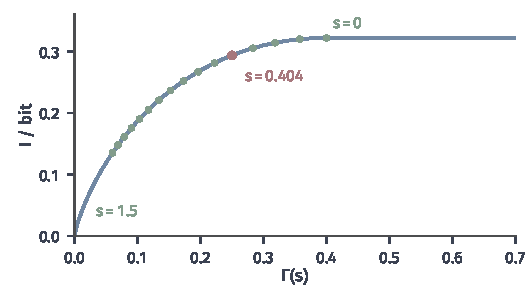
\includegraphics[width=90mm]{figures/07-probability/06-channel-coding/matplotlib/dcc-ba-cost/figure.pdf}
 \caption{Z信道、成本$c(0)=0$、$c(1)=1$时带乘子的Blahut–Arimoto迭代。蓝线为容量—成本函数的解析式，绿点为$s=0,0.1,\dots,1.5$各自迭代$400$轮得到的$(\Gamma(s),I)$，红点为二分求得的$s\approx0.404$，对应预算$\Gamma=0.25$。}
 \label{fig:dcc-ba-cost}
\end{BookInlineFigure}

带约束时，误差保证也要相应修改。上界来自弱对偶~\eqref{eq:dcc-weak-duality}：用定理~\ref{thm:dcc-kkt}中的恒等式，对任意$q$有
\[
 I(q)-s\sum_xq(x)c(x)\leq\max_x\bigl[D_{\mathrm{KL}}(W_x\Vert p_t)-s\,c(x)\bigr] ,
\]
所以
\[
 C(\Gamma)\leq\max_x\bigl[D_t(x)-s\,c(x)\bigr]+s\Gamma ,
\]
对任意$s\geq0$与任意一轮都成立。下界是当前输入的互信息$I(q_t)$，但只有在$\sum_xq_t(x)c(x)\leq\Gamma$时才算数：二分得到的$s$只使预算近似满足，若$q_t$略微超支，它的互信息不是$C(\Gamma)$的下界。所以报告结果时要同时核对实际的平均成本，必要时把$s$稍微调大，换取一个严格可行的输入。


\section{本章小结}
\label{sec:dcc-summary}

本章研究有限字母表上、编码器不使用反馈的离散无记忆信道。信道由转移矩阵$\bm{W}$给出，发送端能选择的是输入分布与码本；可靠传输的含义是码长增长时错误概率趋于零，速率按比特每次信道使用计量。

\paragraph{主要结论}
\begin{itemize}
 \item 容量公式：$C=\max_qI(q)$。$I(q)$是单纯形上的连续凹函数，最大值存在，最优输出分布唯一；最优输入由条件~\eqref{eq:dcc-kkt}刻画：被使用的输入的散度$D_{\mathrm{KL}}(W_x\Vert p^{*})$都等于$C$，未使用的不超过$C$。对任意输出分布$r$，$\max_xD_{\mathrm{KL}}(W_x\Vert r)$是容量的上界。

 \item 块的信息：无记忆与无反馈保证$I(X^n;Y^n)\leq nC$，独立使用最优输入达到等号。

 \item 编码定理：码率$R<C$时，随机码本加联合典型解码使平均错误趋于零，删去一半消息后最大错误也趋于零；码率$R>C$时，Fano不等式与数据处理给出$P_{\mathrm{e}}\geq1-C/R-1/(nR)$，错误不能趋于零。定理对$R=C$及有限块长不作承诺。

 \item 二元信道：二元对称信道$C=1-h_2(p)$，二元擦除信道$C=1-\varepsilon$；均匀输入最优来自交换对称性，Z信道的最优输入是$0.4$。已知错误位置的擦除比未知位置的翻转损失少，差值$h_2(p)-p$是定位错误的代价。

 \item 成本约束：逐条码字的预算下，容量是容量—成本函数$C(\Gamma)$，它单调、凹，切线斜率是预算的边际价值；可达性需要为预算留出余量，预算等于最小成本时改用受限字母表。

 \item 数值计算：Blahut–Arimoto迭代按$2^{D_{\mathrm{KL}}(W_x\Vert p_t)}$乘性地重新加权输入，每轮给出严格的上下界，下界误差不超过$D_{\mathrm{KL}}(q^{*}\Vert q_0)/(T+1)$；初始分布须有完整支撑，停止依据是上下界之差而不是迭代的变化量。
\end{itemize}

\paragraph{对比}
本章有几组容易混淆的概念，表~\ref{tab:dcc-summary-contrast}把它们并列。

\begin{BookInlineTable}
 \centering
 \caption{本章几组相邻概念的区别。}
 \label{tab:dcc-summary-contrast}
 \begin{tabular}{p{18mm}p{39mm}p{39mm}}
  \toprule
  对象 & 前者 & 后者 \\
  \midrule
  两个容量 & $C_{\mathrm{op}}$：可靠码率的上确界 & $C$：单次互信息的最大值 \\
  两种错误 & 平均错误：均匀消息下的错误率 & 最大错误：每条消息的保证 \\
  定理两向 & 可达性：存在好码，不给构造 & 逆定理：对一切码成立的限制 \\
  两种损坏 & 翻转：位置未知，$1-h_2(p)$ & 擦除：位置可见，$1-\varepsilon$ \\
  两种成本 & 期望成本：输入分布的约束 & 逐条预算：每条码字的约束 \\
  两种停止 & 迭代变化小：不是证书 & $U_t-L_t$小：严格的误差保证 \\
  \bottomrule
 \end{tabular}
\end{BookInlineTable}

容量回答“最多能多快”，没有回答“给定块长需要多少冗余”和“怎样以可承受的计算量编码与解码”。随机码本不可存储，典型性解码要搜索指数多个码字；有限长度的纠错构造与性能比较由第~\ref{chap:channel-codes}章展开。下一章先把输入字母从有限集合换成受功率限制的实数，研究高斯噪声下的容量，见第~\ref{chap:gaussian-channel-capacity}章。


\chapter{高斯信道的容量}
\label{chap:gaussian-channel-capacity}

一条线路每次传送一个实数幅值，接收端读到的是幅值加上一个方差为$1$的高斯噪声。发送设备的平均功率不能超过$3$，即每次传送的幅值平方平均不超过$3$。每次使用这条线路，最多能可靠地送出多少比特？若可以把幅值放得任意大，噪声就无关紧要，问题没有意义；正是功率预算与噪声的比例决定了答案。本章证明这个答案是
\[
 \frac12\log_2\Bigl(1+\frac{3}{1}\Bigr)=1\ \text{比特每次使用}.
\]

与第~\ref{chap:discrete-channel-capacity}章相比，困难在于输入和输出都是连续的。输入分布不再构成有限维单纯形，熵要换成可以为负的微分熵，可达性证明中数典型序列的办法也不能照搬。本章用三样东西克服这些困难：固定方差时高斯分布的熵最大，信道条件密度与输出密度之比的对数，以及随块长增大而集中的噪声能量。

全章按模型从简单到复杂推进。第~\ref{sec:gcc-channel}节写清加性高斯噪声模型和逐条码字的功率约束，并用球的体积比猜出容量公式。第~\ref{sec:gcc-scalar}节求单次使用的最大互信息，证明它就是可靠传输的速率极限。第~\ref{sec:gcc-parallel}节研究几个噪声不同的分量共享一个预算时怎样分配功率，得到注水规则。第~\ref{sec:gcc-correlated}节用正交变换把相关噪声化为独立分量，并说明白化时预算怎样随之改变。

本章沿用第~\ref{chap:discrete-channel-capacity}章的块码、码率、错误概率与可达速率的定义，所用的微分熵、互信息、数据处理不等式与Fano不等式取自第~\ref{chap:information-measures}章，固定方差下的高斯熵上界与反注水取自第~\ref{chap:rate-distortion}章。对数以2为底，信息量以比特计；容量的单位是比特每次信道使用，平行与相关模型中一次使用指一次向量输入。

\section{高斯信道}
\label{sec:gcc-channel}

第~\ref{chap:discrete-channel-capacity}章的信道只有有限个输入和输出。线路上实际传送的常常是一个连续的幅值，例如一个电压；接收端读到的是这个幅值加上一份随机扰动。扰动通常是许多微小独立因素的叠加，由第~\ref{chap:central-limit-theorem}章的中心极限定理，用高斯分布描述它是自然的近似。这一节先写清模型和编码的规则，再说明为什么必须限制输入的功率，最后用几何图景猜出容量公式。

\paragraph{加性高斯噪声模型}
输入、输出都取实数值，每次使用信道，输出等于输入加上一个独立的高斯噪声。

\begin{definition}[高斯信道]
\label{def:gcc-channel}
设$\sigma^2>0$。\term{高斯信道}（Gaussian channel）在第$i$次使用时把实数输入$x_i$变成输出
\begin{equation}
 Y_i=x_i+Z_i,\qquad i=1,\dots,n,
 \label{eq:gcc-channel}
\end{equation}
其中$Z_1,\dots,Z_n$独立同分布，$Z_i\sim\mathcal{N}(0,\sigma^2)$，并且与要传送的消息、与编码器选出的输入相互独立。
\end{definition}

记$g_v$为$\mathcal{N}(0,v)$的密度，
\begin{equation}
 g_v(t)=\frac{1}{\sqrt{2\pi v}}\exp\Bigl(-\frac{t^2}{2v}\Bigr),\qquad v>0 .
 \label{eq:gcc-gauss-density}
\end{equation}
给定输入块$x^n=(x_1,\dots,x_n)$，输出块$Y^n$的条件密度是各坐标密度之积，
\begin{equation}
 p(y^n\mid x^n)=\prod_{i=1}^{n}g_{\sigma^2}(y_i-x_i) .
 \label{eq:gcc-block-density}
\end{equation}
这就是第~\ref{chap:discrete-channel-capacity}章无记忆性的连续版本：转移矩阵的乘积换成了条件密度的乘积，各次使用的噪声互不影响。条件密度的含义取自第~\ref{chap:conditional-distributions}章。

与离散信道相比，有两处不同。第一，输入字母表是整条实轴，不能在有限个分布的单纯形上做优化；第二，任意两个输入都可能产生同一个输出，输出不会只落在有限个位置上。图~\ref{fig:gcc-channel-model}画出整块传输的过程。

\begin{BookInlineFigure}
 \centering
 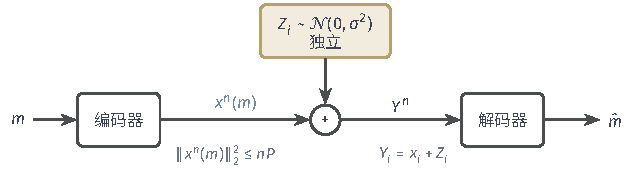
\includegraphics[width=107mm]{figures/07-probability/06-channel-coding/tikz/gcc-channel-model/figure.pdf}
 \caption{高斯信道上的块传输。编码器把消息$m$映成实数码字$x^n(m)$（蓝），它的能量不超过$nP$；每个坐标加上独立的噪声$Z_i\sim\mathcal{N}(0,\sigma^2)$（黄框），解码器根据输出块$Y^n$判决$\hat{m}$。}
 \label{fig:gcc-channel-model}
\end{BookInlineFigure}

\paragraph{不限制幅值时}
先看单次使用、只发两种消息的情形。发送$+A$或$-A$，接收端看输出的符号：输出为正判为$+A$，否则判为$-A$。发送$+A$而判错，需要噪声小于$-A$，概率是
\[
 \mathbb{P}(Z<-A)=\Phi\Bigl(-\frac{A}{\sigma}\Bigr) ,
\]
其中$\Phi$是标准高斯分布函数。取$\sigma=1$，$A=1$时这个概率是$0.159$，$A=3$时降到$0.00135$。图~\ref{fig:gcc-two-point}画出两种情形下的两条输出密度：幅值越大，两条钟形分得越开，重叠的尾部越小。

\begin{BookInlineFigure}
 \centering
 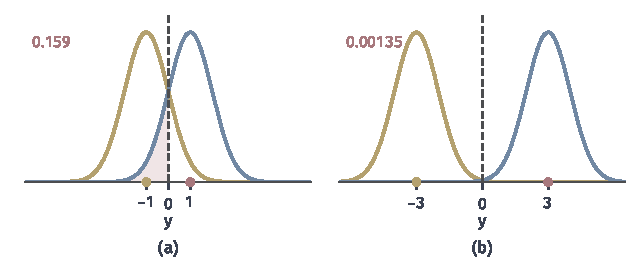
\includegraphics[width=108mm]{figures/07-probability/06-channel-coding/matplotlib/gcc-two-point/figure.pdf}
 \caption{两点输入$\pm A$经过$\sigma^2=1$的高斯噪声。黄线是发送$-A$时的输出密度，蓝线是发送$+A$时的输出密度，虚线是判决门限$0$，红色阴影是发送$+A$而判错的概率。(a)$A=1$，错误概率$0.159$。(b)$A=3$，错误概率$0.00135$。}
 \label{fig:gcc-two-point}
\end{BookInlineFigure}

幅值不受限制时，可靠传输没有上限。把间距固定为$d$，在实轴上放$K$个等距的输入点，每个点被判错的概率不超过$2\Phi(-d/(2\sigma))$，只要$d$足够大，这个概率可以任意小，而$K$可以任意大。于是每次使用可以近乎无错地送出$\log_2K$比特，$K$没有上界。同理，若$\sigma^2=0$，任意两个不同的实数都能被区分，一次使用就能送出任意多的比特。所以有意义的问题必须同时有两个前提：噪声方差为正，输入的幅值受到预算约束。

\paragraph{功率约束下的块码}
实际的发射设备受能量或平均功率的限制。约束加在每一条码字上：

\begin{definition}[功率约束下的块码]
\label{def:gcc-code}
设$P\geq0$。高斯信道上满足\term{功率约束}（power constraint）$P$的$(M,n)$码由编码器$f:\{1,\dots,M\}\to\mathbb{R}^n$与可测的解码器$g:\mathbb{R}^n\to\{1,\dots,M\}$组成，码字$x^n(m)=f(m)$对每条消息都满足
\begin{equation}
 \lVert x^n(m)\rVert_2^2=\sum_{i=1}^{n}x_i(m)^2\leq nP,\qquad m=1,\dots,M .
 \label{eq:gcc-power}
\end{equation}
\end{definition}

码率、条件错误概率、平均错误概率、最大错误概率和可达速率都沿用第~\ref{chap:discrete-channel-capacity}章的定义，只是把对输出块的求和换成对条件密度~\eqref{eq:gcc-block-density}的积分：
\begin{equation}
 \lambda_m=\int_{\{y^n:\,g(y^n)\neq m\}}p\bigl(y^n\mid x^n(m)\bigr)\,\mathrm{d}y^n ,
 \qquad P_{\mathrm{e}}=\frac1M\sum_{m=1}^{M}\lambda_m .
 \label{eq:gcc-errors}
\end{equation}
称$R$为功率$P$下的可达速率，若存在一列满足功率约束$P$的$(M_n,n)$码，$M_n\geq2^{nR}$且$P_{\mathrm{e}}\to0$。可达速率的上确界记作$C_{\mathrm{op}}(P)$。本章用$P$表示功率；分布写作带下标的$P_X$，概率写作$\mathbb{P}$，平均错误概率写作$P_{\mathrm{e}}$，三者不会混淆。

约束~\eqref{eq:gcc-power}有三点需要读清。

第一，它是沿一条码字的时间平均：$\frac1n\sum_ix_i(m)^2\leq P$。同一条码字可以在某些位置用大幅值、在另一些位置用小幅值，只要总能量不超预算。

第二，它对每一条码字分别成立，不允许一条码字超支、由另一条码字的节省来补偿。若只要求$\frac1M\sum_m\lVert x^n(m)\rVert_2^2\leq nP$，约束就变弱了。第~\ref{sec:gcc-coding}小节的逆定理说明，即使在这种较弱的约束下，速率也不能超过同一个上限。

第三，它是第~\ref{chap:discrete-channel-capacity}章输入成本约束的连续类比：成本函数取$c(x)=x^2$，预算取$\Gamma=P$。不同的是输入字母表不再有限，那里依赖有限单纯形紧性的论证都要重做。

$P=0$时，每条码字只能是零向量，不同消息的码字相同，只有$M=1$的码能做到无错，所以$C_{\mathrm{op}}(0)=0$。下文讨论容量公式时通常假设$P>0$，并在结论中注明端点。

\paragraph{噪声向量的长度}
把整块输出看成$\mathbb{R}^n$中的一个点，可以得到一幅几何图景。先看噪声向量$Z^n$的长度。由于$Z_i^2$独立同分布，期望为$\sigma^2$，第~\ref{chap:laws-of-large-numbers}章的弱大数律给出
\[
 \frac1n\lVert Z^n\rVert_2^2=\frac1n\sum_{i=1}^{n}Z_i^2\xrightarrow{\mathbb{P}}\sigma^2 .
\]
也就是说，块长很大时噪声向量的长度几乎总接近$\sqrt{n\sigma^2}$：$n$维高斯噪声集中在一个薄球壳上，而不是均匀地填满一个球。

图~\ref{fig:gcc-noise-norm}画出$\sigma^2=1$时$\lVert Z^n\rVert_2^2/n$的精确密度，它是$\chi^2_n$分布除以$n$。$\lVert Z^n\rVert_2^2/n$落在$[0.8,1.2]$中的概率，$n=4$时是$0.217$，$n=32$时是$0.579$，$n=256$时是$0.976$。

\begin{BookInlineFigure}
 \centering
 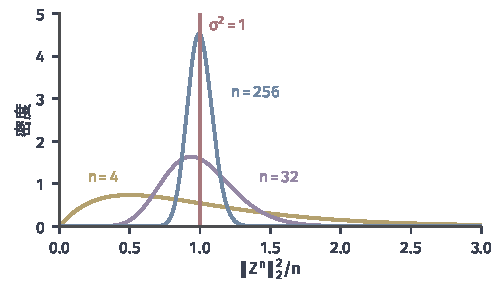
\includegraphics[width=84mm]{figures/07-probability/06-channel-coding/matplotlib/gcc-noise-norm/figure.pdf}
 \caption{$\sigma^2=1$时噪声向量的平均平方长度$\lVert Z^n\rVert_2^2/n$的密度，即$\chi^2_n/n$。黄、紫、蓝三条曲线分别对应$n=4,32,256$，红线是$\sigma^2=1$。块长越大，长度越集中在$\sqrt{n\sigma^2}$附近。}
 \label{fig:gcc-noise-norm}
\end{BookInlineFigure}

输出向量也有同样的现象。设码字满足$\lVert x^n\rVert_2^2\approx nP$，则
\[
 \frac1n\lVert x^n+Z^n\rVert_2^2=\frac1n\lVert x^n\rVert_2^2+\frac2n\langle x^n,Z^n\rangle+\frac1n\lVert Z^n\rVert_2^2 .
\]
中间的交叉项均值为零，方差为$4\sigma^2\lVert x^n\rVert_2^2/n^2\leq4\sigma^2P/n$，随$n$增大而趋于零；最后一项趋于$\sigma^2$。所以输出几乎总落在半径约$\sqrt{n(P+\sigma^2)}$的球内。

\paragraph{球的计数}
现在可以粗略地数一数能区分多少条消息。每条码字的输出集中在以码字为中心、半径约$\sqrt{n\sigma^2}$的小球附近；所有输出都在半径约$\sqrt{n(P+\sigma^2)}$的大球内。要从输出唯一认出码字，各个小球应当基本不重叠，于是码字数至多约为两球体积之比：
\[
 \frac{\bigl(\sqrt{n(P+\sigma^2)}\bigr)^{n}}{\bigl(\sqrt{n\sigma^2}\bigr)^{n}}
 =\Bigl(1+\frac{P}{\sigma^2}\Bigr)^{n/2} .
\]
这里用到了$n$维球的体积与半径的$n$次方成正比，比例常数在两球之间消去。取以2为底的对数再除以$n$，每次使用至多约送出
\[
 \frac12\log_2\Bigl(1+\frac{P}{\sigma^2}\Bigr)\ \text{比特}.
\]

全章的标量例子取$\sigma^2=1$，$P=3$。两球半径之比是$\sqrt{4}=2$，$n$维体积之比是$2^n$，每次使用约$1$比特。图~\ref{fig:gcc-sphere-packing}在平面上画出这幅图景；为了画得下，图中取$P/\sigma^2=8$。

\begin{BookInlineFigure}
 \centering
 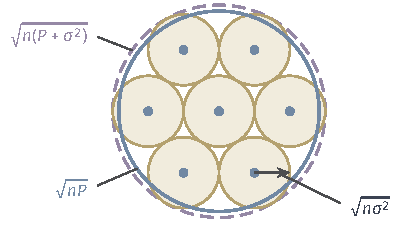
\includegraphics[width=68mm]{figures/07-probability/06-channel-coding/tikz/gcc-sphere-packing/figure.pdf}
 \caption{球的计数在平面上的示意（$n=2$，$P/\sigma^2=8$）。蓝点是码字，位于半径$\sqrt{nP}$的蓝色圆内；黄色小圆是半径$\sqrt{n\sigma^2}$的噪声球；所有输出落在半径$\sqrt{n(P+\sigma^2)}$的紫色虚线圆内。两圆面积之比是$9$，图中放下了$7$个互不重叠的噪声球。}
 \label{fig:gcc-sphere-packing}
\end{BookInlineFigure}

这个计数是启发，不是证明。体积之比只给出码字数的上限的猜测：它没有说明小球能否真的几乎不重叠地排满大球，也没有处理输出落在小球之外的情形。平面上的排列已经显示圆不能恰好铺满，图中$7$个小球只占大圆面积的$7/9$。下一节不再直接排列小球，而是先在单次使用上求互信息的最大值，再用随机选取的码字证明这个值可达；结果与上面的猜测一致。


\section{标量容量}
\label{sec:gcc-scalar}

球的计数猜出了$\frac12\log_2(1+P/\sigma^2)$。仿照第~\ref{chap:discrete-channel-capacity}章，严格的做法分两步：先把单次使用的输入看成随机变量$X$，在功率预算$\mathbb{E}[X^2]\leq P$下最大化互信息$I(X;Y)$；再证明这个最大值恰好是满足约束~\eqref{eq:gcc-power}的块码所能达到的速率极限。

\paragraph{单次使用的优化问题}
设$X$与$Z\sim\mathcal{N}(0,\sigma^2)$独立，$Y=X+Z$。输入不再限于有限个值，它可以是离散的、有密度的或两者混合的任意实值随机变量。互信息按第~\ref{chap:information-measures}章的一般定义理解为联合分布相对于边缘乘积的KL散度，
\[
 I(X;Y)=D_{\mathrm{KL}}\bigl(P_{XY}\,\Vert\,P_X\otimes P_Y\bigr),
\]
本章以比特计，即对数取以2为底。单次使用的优化问题是
\begin{equation}
 C(P)=\sup\bigl\{I(X;Y):\ X\text{与}Z\text{独立},\ \mathbb{E}[X^2]\leq P\bigr\} ,
 \label{eq:gcc-info-capacity}
\end{equation}
称为功率$P$下的信息容量。可行的输入分布组成一个无穷维的集合，这里先写上确界；下面会看到它能被取到。

\subsection{容量上界}
\label{sec:gcc-upper}

上界来自两个事实：输出$Y$的方差受预算控制；方差固定时，高斯分布的微分熵最大。后一个事实在第~\ref{chap:rate-distortion}章研究高斯信源时已经证明，这里重述结论，并回顾它的来源。

\begin{lemma}[固定方差的熵上界]
\label{lem:gcc-max-entropy}
设实值随机变量$Y$有密度$f$，方差$s\in(0,\infty)$，并且微分熵$h(Y)=-\int f\log_2f$有定义且有限。则
\begin{equation}
 h(Y)\leq\frac12\log_2(2\pi\mathrm{e}\,s),
 \label{eq:gcc-max-entropy}
\end{equation}
等号当且仅当$Y$服从高斯分布时成立。
\end{lemma}

回顾其理由：取与$Y$同均值$\mu$、同方差$s$的高斯密度$q$。$-\log_2q(y)$是$(y-\mu)^2$的一次函数，它在$Y$下的期望只依赖均值和方差，等于$\frac12\log_2(2\pi\mathrm{e}s)$。于是
\[
 0\leq D_{\mathrm{KL}}(f\Vert q)=-h(Y)+\frac12\log_2(2\pi\mathrm{e}\,s),
\]
等号当且仅当$f=q$几乎处处成立。高斯分布本身的微分熵正是右端，所以$h(Z)=\frac12\log_2(2\pi\mathrm{e}\sigma^2)$。

要把引理用在输出$Y$上，先要确认$Y$有密度、熵有限，并且互信息可以写成两个微分熵之差。这些都由“输入二阶矩有限、噪声是独立的高斯变量”保证。

\begin{lemma}[输出的密度与互信息]
\label{lem:gcc-output}
设$\mathbb{E}[X^2]<\infty$，$Z\sim\mathcal{N}(0,\sigma^2)$与$X$独立，$Y=X+Z$。则
\begin{enumerate}
 \item $Y$有密度$f_Y(y)=\mathbb{E}\bigl[g_{\sigma^2}(y-X)\bigr]$，并且$0<f_Y(y)\leq(2\pi\sigma^2)^{-1/2}$；
 \item $\mathbb{E}[Y^2]=\mathbb{E}[X^2]+\sigma^2$，并且$Y$的方差等于$X$的方差加上$\sigma^2$；
 \item $h(Y)$有限，并且
 \begin{equation}
  I(X;Y)=h(Y)-h(Z)=h(Y)-\frac12\log_2(2\pi\mathrm{e}\sigma^2) .
  \label{eq:gcc-mi-entropy}
 \end{equation}
\end{enumerate}
\end{lemma}

\begin{proof}
第一条。由独立性和Fubini定理，对任意$t$，
\[
 \mathbb{P}(Y\leq t)=\mathbb{E}\Bigl[\int_{-\infty}^{t}g_{\sigma^2}(y-X)\,\mathrm{d}y\Bigr]
 =\int_{-\infty}^{t}\mathbb{E}\bigl[g_{\sigma^2}(y-X)\bigr]\,\mathrm{d}y ,
\]
所以$f_Y(y)=\mathbb{E}[g_{\sigma^2}(y-X)]$是$Y$的密度。被平均的函数取值在$(0,(2\pi\sigma^2)^{-1/2}]$中，平均值也在这个范围内。

第二条。$X$与$Z$独立且$\mathbb{E}[Z]=0$，所以$\mathbb{E}[XZ]=0$，展开$(X+Z)^2$取期望即得前一式；独立变量的方差可加，即得后一式。

第三条。先说明$\log_2f_Y(Y)$可积。上界由第一条给出：$\log_2f_Y(y)\leq-\frac12\log_2(2\pi\sigma^2)$。下界用Jensen不等式：$\ln$是凹函数，
\[
 \begin{aligned}
  \ln f_Y(y)&=\ln\mathbb{E}\bigl[g_{\sigma^2}(y-X)\bigr]\geq\mathbb{E}\bigl[\ln g_{\sigma^2}(y-X)\bigr]\\
  &=-\frac12\ln(2\pi\sigma^2)-\frac{\mathbb{E}[(y-X)^2]}{2\sigma^2} .
 \end{aligned}
\]
再用$(y-x)^2\leq2y^2+2x^2$，得到
\[
 \ln f_Y(y)\geq-\frac12\ln(2\pi\sigma^2)-\frac{y^2+\mathbb{E}[X^2]}{\sigma^2} .
\]
两边夹住，$\lvert\ln f_Y(Y)\rvert$不超过常数加$Y^2/\sigma^2$，而$\mathbb{E}[Y^2]<\infty$，所以$h(Y)=-\mathbb{E}[\log_2f_Y(Y)]$有限。

再看互信息。对可测集$A,B$，由独立性，
\[
 \begin{aligned}
  P_{XY}(A\times B)&=\mathbb{E}\Bigl[\mathbf{1}_{A}(X)\int_Bg_{\sigma^2}(y-X)\,\mathrm{d}y\Bigr]\\
  &=\iint_{A\times B}\frac{g_{\sigma^2}(y-x)}{f_Y(y)}\,P_X(\mathrm{d}x)\,f_Y(y)\,\mathrm{d}y .
 \end{aligned}
\]
所以$r(x,y)=g_{\sigma^2}(y-x)/f_Y(y)$是$P_{XY}$相对于$P_X\otimes P_Y$的密度。KL散度是$\log_2r$在$P_{XY}$下的期望；在$(X,Y)$处$y-x=Z$，于是
\[
 I(X;Y)=\mathbb{E}\bigl[\log_2g_{\sigma^2}(Z)\bigr]-\mathbb{E}\bigl[\log_2f_Y(Y)\bigr]=-h(Z)+h(Y) .
\]
两个期望都有限，拆开是合法的。
\end{proof}

证明中密度$r$的存在性用的是卷四的Radon–Nikodym框架，可参考\BookChapterRef{chap:measure-densities}{卷四第8章“测度的密度”}。式~\eqref{eq:gcc-mi-entropy}的读法与离散情形相同：$h(Y)$度量输出的总分散程度，$h(Z)$是知道输入以后仍然剩下的分散程度，两者之差是观测输出对输入不确定性的减少。噪声加在输入之上、与输入独立，所以“知道输入后剩下的分散”总是同一个$h(Z)$，与输入怎样分布无关。

微分熵本身可以为负，单独一项没有“需要多少比特”的含义。例如$\sigma^2=0.01$时，
\[
 h(Z)=\frac12\log_2(2\pi\mathrm{e}\cdot0.01)=-1.27\ \text{比特}.
\]
这不妨碍式~\eqref{eq:gcc-mi-entropy}：把输入、输出同时乘以常数$a\neq0$，$h(Y)$和$h(Z)$都增加$\log_2\lvert a\rvert$，差不变，与互信息在可逆变换下不变一致。引理的第三条之所以要先证明$h(Y)$有限，正是为了保证这个差不是“无穷减无穷”。

\begin{theorem}[互信息的上界]
\label{thm:gcc-upper}
设$Z\sim\mathcal{N}(0,\sigma^2)$，$\sigma^2>0$，$X$与$Z$独立且$\mathbb{E}[X^2]\leq P$。则
\begin{equation}
 I(X;X+Z)\leq\frac12\log_2\Bigl(1+\frac{P}{\sigma^2}\Bigr) .
 \label{eq:gcc-upper}
\end{equation}
\end{theorem}

\begin{proof}
由引理~\ref{lem:gcc-output}，$Y=X+Z$有密度，$h(Y)$有限，方差满足
\[
 \sigma^2\leq\operatorname{Var}(Y)\leq\mathbb{E}[Y^2]=\mathbb{E}[X^2]+\sigma^2\leq P+\sigma^2 .
\]
方差为正且有限，引理~\ref{lem:gcc-max-entropy}适用，再利用$\log_2$单调递增，得到
\[
 h(Y)\leq\frac12\log_2\bigl(2\pi\mathrm{e}\operatorname{Var}(Y)\bigr)\leq\frac12\log_2\bigl(2\pi\mathrm{e}(P+\sigma^2)\bigr) .
\]
代入式~\eqref{eq:gcc-mi-entropy}，两项中的$2\pi\mathrm{e}$相消，
\[
 I(X;Y)\leq\frac12\log_2\bigl(2\pi\mathrm{e}(P+\sigma^2)\bigr)-\frac12\log_2(2\pi\mathrm{e}\sigma^2)=\frac12\log_2\frac{P+\sigma^2}{\sigma^2} .
\]
\end{proof}

定理的三个条件各有作用。$\sigma^2>0$保证$Y$有密度、$h(Z)$有限；若$\sigma^2=0$，$h(Z)$不存在，而上一节已经看到容量没有上限。$X$与$Z$独立保证知道输入后剩下的熵恰好是$h(Z)$，也保证方差相加。$\mathbb{E}[X^2]\leq P$只控制二阶矩，它同时约束了均值和方差。二阶矩等于均值的平方加方差，而输出熵只依赖于$Y$的分布形状和分散程度，平移不改变微分熵；所以均值非零的输入不带来任何好处，只是把一部分预算花在了平移上。

\paragraph{例：同一预算下的三种输入}
取$\sigma^2=1$，$P=3$。噪声的熵是$h(Z)=\frac12\log_2(2\pi\mathrm{e})=2.047$比特，输出熵的上界是$\frac12\log_2(8\pi\mathrm{e})=3.047$比特，所以任何满足预算的输入都有$I(X;Y)\leq1$比特。

比较三种功率都等于$3$的输入：等概率取$\pm\sqrt3$的二点输入，$[-3,3]$上的均匀输入，以及$\mathcal{N}(0,3)$。数值积分给出
\[
 I_{\text{二点}}=0.845,\qquad I_{\text{均匀}}=0.972,\qquad I_{\text{高斯}}=1.000 .
\]
图~\ref{fig:gcc-output-entropy}画出三种输入对应的输出密度。三者方差相同，二点输入的输出是两个钟形的叠加，中间凹下；均匀输入的输出顶部较平；只有高斯输入的输出仍是高斯形状。方差相同时形状越接近高斯，输出熵越大，互信息也越大。

\begin{BookInlineFigure}
 \centering
 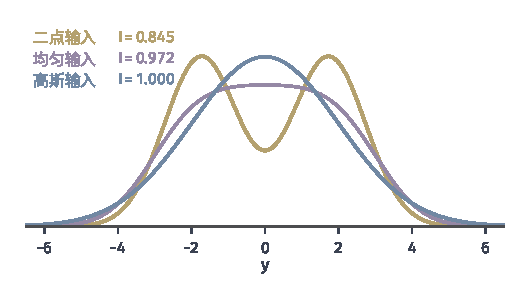
\includegraphics[width=88mm]{figures/07-probability/06-channel-coding/matplotlib/gcc-output-entropy/figure.pdf}
 \caption{$\sigma^2=1$时，三种功率都为$3$的输入经过信道后的输出密度：二点输入$\pm\sqrt3$（黄），$[-3,3]$上的均匀输入（紫），$\mathcal{N}(0,3)$（蓝）。三条输出的方差都是$4$，图中给出对应的互信息（比特）。}
 \label{fig:gcc-output-entropy}
\end{BookInlineFigure}

\subsection{最优输入}
\label{sec:gcc-optimal-input}

上界~\eqref{eq:gcc-upper}的证明中有两处放大：$\operatorname{Var}(Y)\leq P+\sigma^2$，以及固定方差的熵上界。要使两处都取等号，输出必须是方差恰为$P+\sigma^2$的高斯变量。独立高斯变量之和仍是高斯变量（第~\ref{chap:random-variable-transformations}章），所以取$X\sim\mathcal{N}(0,P)$即可：此时$Y\sim\mathcal{N}(0,P+\sigma^2)$。

\begin{theorem}[高斯信道的信息容量]
\label{thm:gcc-capacity}
设$\sigma^2>0$，$P\geq0$。式~\eqref{eq:gcc-info-capacity}中的上确界可以取到，并且
\begin{equation}
 C(P)=\frac12\log_2\Bigl(1+\frac{P}{\sigma^2}\Bigr)\quad\text{比特每次信道使用}.
 \label{eq:gcc-capacity}
\end{equation}
达到最大值的输入分布唯一，是$\mathcal{N}(0,P)$（$P=0$时理解为恒等于零的输入）。
\end{theorem}

\begin{proof}
上界由定理~\ref{thm:gcc-upper}给出。$P>0$时取$X\sim\mathcal{N}(0,P)$与$Z$独立，$Y\sim\mathcal{N}(0,P+\sigma^2)$，由式~\eqref{eq:gcc-mi-entropy}，
\[
 I(X;Y)=\frac12\log_2\bigl(2\pi\mathrm{e}(P+\sigma^2)\bigr)-\frac12\log_2(2\pi\mathrm{e}\sigma^2)=C(P) .
\]
$P=0$时只能$X=0$，$Y=Z$，互信息为零，与公式一致。

再证唯一性，设$P>0$且某个可行输入$X$达到$C(P)$。上界证明中的两处不等式都必须取等号：$Y$的方差等于$P+\sigma^2$，且$Y$是高斯变量。$Y$的方差是$X$的方差加$\sigma^2$，所以
\[
 \operatorname{Var}(X)=P\geq\mathbb{E}[X^2]=(\mathbb{E}X)^2+\operatorname{Var}(X),
\]
于是$\mathbb{E}[X]=0$，$Y\sim\mathcal{N}(0,P+\sigma^2)$。用第~\ref{chap:weak-convergence-of-distributions}章的特征函数，独立和的特征函数是乘积：
\[
 \mathrm{e}^{-(P+\sigma^2)t^2/2}=\phi_Y(t)=\phi_X(t)\,\phi_Z(t)=\phi_X(t)\,\mathrm{e}^{-\sigma^2t^2/2} .
\]
$\phi_Z(t)$处处不为零，两边相除得$\phi_X(t)=\mathrm{e}^{-Pt^2/2}$。特征函数唯一确定分布，所以$X\sim\mathcal{N}(0,P)$。
\end{proof}

比值$P/\sigma^2$称为\term{信噪比}（signal-to-noise ratio，SNR）。容量只依赖信噪比：把输出除以$\sigma$得到噪声方差为$1$、功率为$P/\sigma^2$的信道，接收端可以随时这样做或撤销，传输能力不变。工程上常用分贝表示信噪比，即$10\log_{10}(P/\sigma^2)$。

\paragraph{读容量公式}
公式~\eqref{eq:gcc-capacity}的单位是比特每次实值信道使用。全章的例子$P/\sigma^2=3$给出
\[
 C=\tfrac12\log_2 4=1\ \text{比特每次},
\]
与球的计数一致。把信噪比提到$15$，$1+P/\sigma^2$从$4$变成$16$，容量变成$2$比特：功率增加到五倍，容量只增加一倍。

容量是信噪比的凹函数，图~\ref{fig:gcc-capacity-curve}分两段读它。信噪比很小时，由$\ln(1+u)\leq u$且$u\to0$时二者之比趋于$1$，
\[
 C(P)\leq\frac{\log_2\mathrm{e}}{2}\cdot\frac{P}{\sigma^2},\qquad
 \frac{C(P)}{P/\sigma^2}\to\frac{\log_2\mathrm{e}}{2}\approx0.721\quad(P\to0) .
\]
低信噪比时容量与功率近似成正比，每单位信噪比约值$0.721$比特。信噪比很大时，$\log_2(1+u)-\log_2u\to0$，容量接近$\frac12\log_2(P/\sigma^2)$，功率每增加到四倍（约$6.02$分贝），容量只多$1$比特。

\begin{BookInlineFigure}
 \centering
 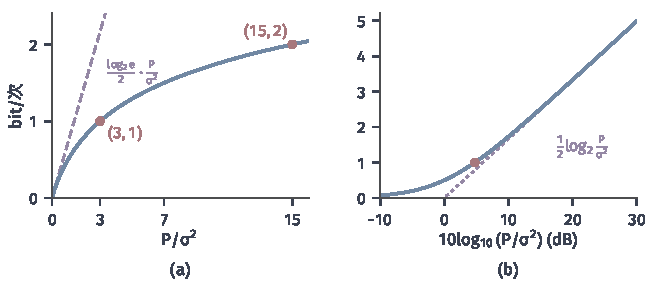
\includegraphics[width=110mm]{figures/07-probability/06-channel-coding/matplotlib/gcc-capacity-curve/figure.pdf}
 \caption{标量高斯信道的容量$C=\frac12\log_2(1+P/\sigma^2)$（蓝）。(a)线性横轴，红点是$(3,1)$和$(15,2)$，紫色虚线是低信噪比时的切线$\frac{\log_2\mathrm{e}}{2}\cdot\frac{P}{\sigma^2}$。(b)横轴为分贝，紫色点线是高信噪比的渐近线$\frac12\log_2(P/\sigma^2)$，斜率约为每$6.02$分贝$1$比特。}
 \label{fig:gcc-capacity-curve}
\end{BookInlineFigure}

\paragraph{有限个输入值的代价}
高斯输入要用到所有实数幅值。若只允许有限个输入值，互信息会低于$C(P)$。等概率二点输入$\pm\sqrt{P}$的互信息不超过$1$比特，无论功率多大；若接收端只记录输出的正负号，信道变成翻转概率$p=\Phi(-\sqrt{P/\sigma^2})$的二元对称信道，速率降为第~\ref{chap:discrete-channel-capacity}章的$1-h_2(p)$，$h_2$是以比特计的二元熵函数。$P/\sigma^2=3$时，$p=0.0416$，三个数是
\[
 C=1.000,\qquad I_{\text{二点}}=0.845,\qquad 1-h_2(p)=0.750 .
\]

图~\ref{fig:gcc-binary-input}把三条曲线画在一起。低信噪比时三者差距很小，因为容量本来就远小于$1$比特，二点输入已经够用；信噪比升高后，二点输入的曲线停在$1$比特，高斯输入继续增长。符号判决丢掉了输出幅值中的可信度信息，由第~\ref{chap:information-measures}章的数据处理不等式，它只能减少互信息。

\begin{BookInlineFigure}
 \centering
 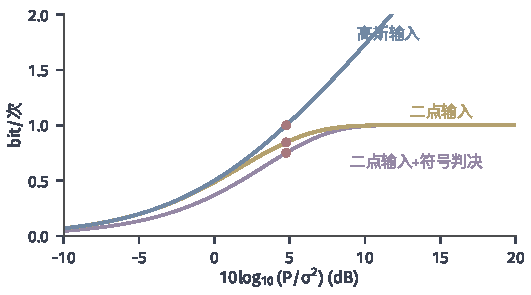
\includegraphics[width=90mm]{figures/07-probability/06-channel-coding/matplotlib/gcc-binary-input/figure.pdf}
 \caption{$\sigma^2=1$时三种传输方式的速率随信噪比（分贝）的变化。蓝：高斯输入，即容量；黄：等概率二点输入，接收端使用实数输出；紫：同样的二点输入，接收端只取输出的正负号。红点对应$P/\sigma^2=3$。}
 \label{fig:gcc-binary-input}
\end{BookInlineFigure}

\paragraph{计量单位}
$C(P)$是每次实值使用的比特数，功率$P$是每次使用的平均能量。改变计量方式时，两者要一起换算。

若每个时刻传送的是一个复数，可以把实部和虚部看成两次实值使用。常见的约定是复噪声的实部与虚部独立，各有方差$\sigma^2/2$，复输入满足$\mathbb{E}\lvert X\rvert^2\leq P$。实部和虚部各分到功率$P/2$时，两次实值使用合计
\[
 2\cdot\frac12\log_2\Bigl(1+\frac{P/2}{\sigma^2/2}\Bigr)=\log_2\Bigl(1+\frac{P}{\sigma^2}\Bigr)\ \text{比特每次复值使用}.
\]
平均分配为什么最优，由第~\ref{sec:gcc-parallel}节的平行信道回答。

若信道每秒使用$m$次，每秒能可靠传送$m\,C(P)$比特，前提是这$m$次使用仍满足本章的模型：噪声独立、方差都是$\sigma^2$，并且$P$指每次使用的功率。若改为给定每秒的总能量，或使用频率改变时噪声方差也随之改变，就要先把这些量折算回每次使用，再代入公式~\eqref{eq:gcc-capacity}。

\subsection{满足功率约束的编码}
\label{sec:gcc-coding}

信息容量是单次使用上的优化值。它是否就是块码的速率极限$C_{\mathrm{op}}(P)$，需要两个方向的证明：低于$C(P)$的速率都可达，高于$C(P)$的速率都不可达。

\begin{theorem}[高斯信道的编码定理]
\label{thm:gcc-coding}
设$\sigma^2>0$，$P>0$。
\begin{enumerate}
 \item 对每个$R<C(P)$，存在一列满足功率约束$P$的$(M_n,n)$码，$M_n\geq2^{nR}$，并且最大错误概率$\lambda_{\max}\to0$。
 \item 任意一列满足功率约束$P$的码，若平均错误概率$P_{\mathrm{e}}\to0$，则$\limsup_{n\to\infty}\frac1n\log_2M_n\leq C(P)$。
\end{enumerate}
因此$C_{\mathrm{op}}(P)=C(P)$；$P=0$时两者都是$0$。
\end{theorem}

\paragraph{为什么不能照搬典型集计数}
第~\ref{chap:discrete-channel-capacity}章的可达性证明数的是典型序列的个数：有限字母表上长为$n$的序列只有有限多个，每个典型序列的概率约为$2^{-nH}$。连续输入下，任何一个具体序列的概率都是零，“个数”没有意义，也不能把$2^{-nH}$中的$H$直接换成可以为负的微分熵。可以保留的是另一样东西：信道条件密度与输出边缘密度之比。下面用它的对数代替典型性。

\paragraph{信息密度}
选一个略低于预算的功率$P'\in(0,P)$，让码字的坐标独立地服从$\mathcal{N}(0,P')$。在这个输入分布下，输出的边缘密度是$g_{P'+\sigma^2}$。

\begin{definition}[信息密度]
\label{def:gcc-info-density}
对输入分布$\mathcal{N}(0,P')$，单次使用的\term{信息密度}（information density）是
\begin{equation}
 i(x;y)=\log_2\frac{g_{\sigma^2}(y-x)}{g_{P'+\sigma^2}(y)} ,
 \label{eq:gcc-info-density}
\end{equation}
长度为$n$的块上的信息密度是逐坐标之和$i_n(x^n;y^n)=\sum_{i=1}^{n}i(x_i;y_i)$。
\end{definition}

$i(x;y)$比较两种解释：$y$是$x$经过噪声得到的，还是与$x$无关地随机出现的。它为正，说明$y$更像由$x$产生。把两个高斯密度代入并展开，
\begin{equation}
 i(x;y)=C(P')+\frac{\log_2\mathrm{e}}{2}\Bigl(\frac{y^2}{P'+\sigma^2}-\frac{(y-x)^2}{\sigma^2}\Bigr) .
 \label{eq:gcc-info-density-explicit}
\end{equation}
信息密度有两个用途，分别对应发送的码字和其余的码字。

第一，对发送的码字及其输出，$i_n$集中在$nC(P')$附近。设$X\sim\mathcal{N}(0,P')$，$Y=X+Z$。此时$Y^2/(P'+\sigma^2)$与$Z^2/\sigma^2$都服从$\chi^2_1$，均值为$1$，所以$\mathbb{E}[i(X;Y)]=C(P')$，这正是式~\eqref{eq:gcc-mi-entropy}的互信息。再算方差：两项的方差都是$2$；$Y$与$Z$是联合高斯的零均值变量，对这样的变量有
\[
 \operatorname{Cov}(Y^2,Z^2)=2\operatorname{Cov}(Y,Z)^2=2\sigma^4 ,
\]
因此
\[
 \operatorname{Var}\Bigl(\frac{Y^2}{P'+\sigma^2}-\frac{Z^2}{\sigma^2}\Bigr)=2+2-\frac{4\sigma^4}{(P'+\sigma^2)\sigma^2}=\frac{4P'}{P'+\sigma^2} .
\]
乘以$(\log_2\mathrm{e}/2)^2$，单次信息密度的方差是
\begin{equation}
 V(P')=\operatorname{Var}\bigl(i(X;Y)\bigr)=(\log_2\mathrm{e})^2\,\frac{P'}{P'+\sigma^2} .
 \label{eq:gcc-info-variance}
\end{equation}
$i_n$是$n$个独立同分布项之和，均值$nC(P')$，方差$nV(P')$。

第二，对与输出无关的码字，$i_n$很少超过高的门限。设$\bar{X}^n$的坐标独立服从$\mathcal{N}(0,P')$，与$Y^n$独立，$Y^n$的坐标独立服从$\mathcal{N}(0,P'+\sigma^2)$。$(\bar{X}^n,Y^n)$的联合密度是乘积$q(x^n,y^n)=f(x^n)\prod_ig_{P'+\sigma^2}(y_i)$，而发送与输出配对时的联合密度是$p(x^n,y^n)=f(x^n)\prod_ig_{\sigma^2}(y_i-x_i)$，$f$是输入块的密度。由定义，二者之比正是
\[
 \frac{q(x^n,y^n)}{p(x^n,y^n)}=2^{-i_n(x^n;y^n)} .
\]
于是对任意$\gamma$，
\begin{equation}
 \mathbb{P}\bigl(i_n(\bar{X}^n;Y^n)>n\gamma\bigr)=\int_{\{i_n>n\gamma\}}2^{-i_n}\,p\leq2^{-n\gamma}\int p=2^{-n\gamma} .
 \label{eq:gcc-change-of-measure}
\end{equation}
这一步把“独立配对”的概率换成“发送配对”的积分，换算因子就是$2^{-i_n}$，在门限以上它不超过$2^{-n\gamma}$。

\paragraph{例：信息密度的两种分布}
取$\sigma^2=1$，$P'=3$。发送配对时$\mathbb{E}[i]=C(3)=1$，$V=(\log_2\mathrm{e})^2\cdot\frac34=1.561$。独立配对时，$\mathbb{E}[(Y-\bar{X})^2]=(P'+\sigma^2)+P'=7$，代入式~\eqref{eq:gcc-info-density-explicit}，
\[
 \mathbb{E}[i(\bar{X};Y)]=1+\frac{\log_2\mathrm{e}}{2}\Bigl(1-7\Bigr)=1-3\log_2\mathrm{e}=-3.33 .
\]
图~\ref{fig:gcc-info-density}画出$n=20$与$n=200$时两种配对的$i_n/n$的直方图。块长增大，两个直方图分别收拢到$1$和$-3.33$；在两者之间放一个门限$\gamma$，发送的码字几乎总在门限之上，独立的码字几乎总在门限之下。

\begin{BookInlineFigure}
 \centering
 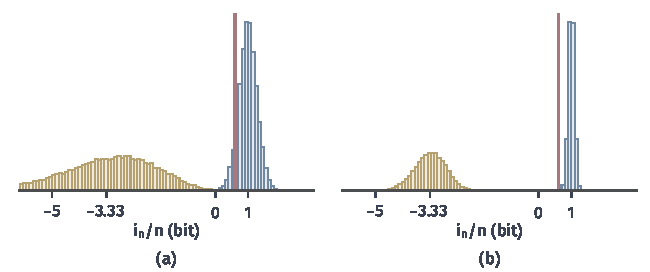
\includegraphics[width=110mm]{figures/07-probability/06-channel-coding/matplotlib/gcc-info-density/figure.pdf}
 \caption{$\sigma^2=1$、码字坐标服从$\mathcal{N}(0,3)$时归一化信息密度$i_n/n$的直方图（种子$7$，每个直方图$20000$对）。蓝：发送的码字与其输出，均值$1$；黄：与输出独立的码字，均值$-3.33$。红线是门限$\gamma=0.6$。(a)$n=20$，蓝色样本有$7.3\%$落在门限以下。(b)$n=200$，没有蓝色样本落在门限以下，也没有黄色样本落在门限以上。}
 \label{fig:gcc-info-density}
\end{BookInlineFigure}

\paragraph{随机码本与阈值判决}
现在构造码。给定$R<C(P)$，由$C$的连续性和严格单调性，可以依次选出
\[
 0<P'<P,\qquad R<\gamma<C(P') .
\]
取$M_n=2^{\lceil nR\rceil+1}$。码本由$M_n$个独立的随机码字$X^n(1),\dots,X^n(M_n)$组成，每个码字的坐标独立服从$\mathcal{N}(0,P')$。解码采用\term{阈值判决}（threshold decoding）：收到$y^n$后，若恰有一个$m$满足$i_n(X^n(m);y^n)>n\gamma$，判为这个$m$；否则判为$1$。

随机码字有可能超过预算，这样的码字不允许发送。分析时采取保守的记账：若$\lVert X^n(m)\rVert_2^2>nP$，就把消息$m$的条件错误概率记为$1$。

\paragraph{例：一次阈值判决}
用一个极小的码本走一遍判决过程。取$\sigma^2=1$，$P'=3$，$n=2$，门限$\gamma=0.6$，即要求$i_2>1.2$。三条码字和收到的输出是
\[
 \begin{gathered}
  x^2(1)=(1.5,-2.0),\quad x^2(2)=(-1.0,1.0),\quad x^2(3)=(2.0,1.5);\\
  y^2=(1.2,-1.4) .
 \end{gathered}
\]
由式~\eqref{eq:gcc-info-density-explicit}，此时
\[
 i(x;y)=1+\frac{\log_2\mathrm{e}}{2}\Bigl(\frac{y^2}{4}-(y-x)^2\Bigr) .
\]
对码字$1$的第一个坐标，$y^2/4=0.36$，$(y-x)^2=0.09$，代入得$1.195$；第二个坐标得$1.094$。三条码字的块信息密度分别是
\[
 i_2(x^2(1);y^2)=2.289,\quad i_2(x^2(2);y^2)=-5.033,\quad i_2(x^2(3);y^2)=-3.915 .
\]
只有码字$1$越过$1.2$，判为消息$1$。码字$3$的第一个坐标与输出也相当接近，信息密度为$0.798$，但第二个坐标相差$2.9$，在噪声标准差为$1$的信道上很不可能，贡献了$-4.713$，整块被否决。块信息密度把各坐标的证据加起来，一个坐标上的偶然吻合抵不过其他坐标上的明显不符。

\paragraph{三类错误}
由对称性，只需分析消息$1$，并对码本的随机性取平均。消息$1$被记为错误，只可能是下面三件事之一发生：
\begin{enumerate}
 \item $E_0$：码字超预算，$\lVert X^n(1)\rVert_2^2>nP$；
 \item $E_1$：发送的码字没有越过门限，$i_n(X^n(1);Y^n)\leq n\gamma$；
 \item $E_2$：某个其他码字越过了门限，即存在$m\neq1$使$i_n(X^n(m);Y^n)>n\gamma$。
\end{enumerate}
三件事都不发生时，恰有消息$1$越过门限，判决正确。三个概率可以分别估计。

$E_0$：$X_i^2$独立同分布，均值$P'$，方差$2P'^2$。由第~\ref{chap:tail-probabilities}章的Chebyshev不等式，
\[
 \mathbb{P}(E_0)=\mathbb{P}\Bigl(\sum_{i=1}^{n}(X_i^2-P')>n(P-P')\Bigr)\leq\frac{2P'^2}{n(P-P')^2} .
\]

$E_1$：$i_n$的均值是$nC(P')$，方差是$nV(P')$，门限$n\gamma$比均值低$n(C(P')-\gamma)$。同样由Chebyshev不等式，
\[
 \mathbb{P}(E_1)\leq\frac{V(P')}{n\bigl(C(P')-\gamma\bigr)^2} .
\]

$E_2$：每个$m\neq1$的码字与发送的码字独立，也与噪声独立，所以与$Y^n$独立，式~\eqref{eq:gcc-change-of-measure}适用。对$M_n-1$个码字用并集界，并利用$M_n\leq2^{nR+2}$，
\[
 \mathbb{P}(E_2)\leq(M_n-1)\,2^{-n\gamma}\leq4\cdot2^{-n(\gamma-R)} .
\]

三项相加，对码本取平均后，消息$1$的记账错误概率不超过
\begin{equation}
 \varepsilon_n=\frac{2P'^2}{n(P-P')^2}+\frac{V(P')}{n\bigl(C(P')-\gamma\bigr)^2}+4\cdot2^{-n(\gamma-R)} ,
 \label{eq:gcc-random-code-bound}
\end{equation}
三项都随$n\to\infty$趋于零。前两项来自大数律，按$1/n$减小；第三项来自门限与码率之间的余量$\gamma-R$，按指数减小。

以$\sigma^2=1$、$P=3$、$R=0.5$为例，取$P'=2.4$，$\gamma=0.7$。此时$C(P')=\frac12\log_2 3.4=0.883$，$V(P')=1.469$。$n=400$时式~\eqref{eq:gcc-random-code-bound}的三项约为
\[
 0.080,\qquad 0.110,\qquad 3\times10^{-24} .
\]
Chebyshev界相当粗：图~\ref{fig:gcc-codeword-energy}的精确计算表明，$n=400$时码字超预算的概率只有$0.00048$，而不是$0.080$。证明只需要这些界趋于零，不需要它们精确。

\begin{BookInlineFigure}
 \centering
 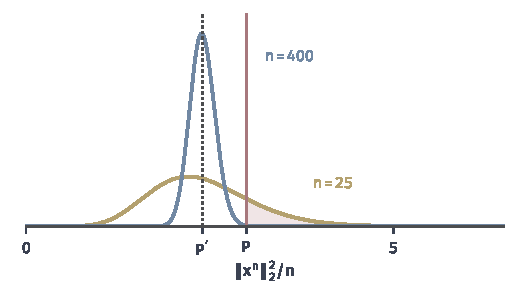
\includegraphics[width=88mm]{figures/07-probability/06-channel-coding/matplotlib/gcc-codeword-energy/figure.pdf}
 \caption{坐标独立服从$\mathcal{N}(0,P')$的随机码字的每坐标能量$\lVert x^n\rVert_2^2/n$的精确密度，$P'=2.4$，预算$P=3$（红线），点线标出$P'$。黄：$n=25$；蓝：$n=400$。红色阴影是超预算的概率，$n=25$时为$0.181$，$n=400$时为$0.00048$。}
 \label{fig:gcc-codeword-energy}
\end{BookInlineFigure}

\paragraph{从随机码本到确定的码}
式~\eqref{eq:gcc-random-code-bound}是对码本取平均的结果。由对称性，每条消息的平均记账错误都相同，所以$\frac1{M_n}\sum_m\tilde{\lambda}_m$对码本的平均也不超过$\varepsilon_n$，其中$\tilde{\lambda}_m$表示消息$m$的记账错误概率。平均值不超过$\varepsilon_n$，至少有一个码本取到不超过$\varepsilon_n$的值；固定这个码本。

这个码本中，记账错误超过$2\varepsilon_n$的消息至多占一半，否则平均值会超过$\varepsilon_n$。删去记账错误最大的一半消息，保留$M_n/2=2^{\lceil nR\rceil}\geq2^{nR}$条，每条都满足$\tilde{\lambda}_m\leq2\varepsilon_n$。当$n$足够大使$2\varepsilon_n<1$时，被保留的码字都不超预算，因为超预算的码字记账错误是$1$。

解码器改为只在保留的码字中做阈值判决。对一条保留的消息，新的错误事件包含在原来的$E_1$与“某个保留的其他码字越过门限”之并中，后者又包含在原来的$E_2$中，所以错误概率不会增加。这样得到的码满足功率约束，码率至少为$R$，最大错误概率不超过$2\varepsilon_n\to0$，定理~\ref{thm:gcc-coding}的第一条得证。

\begin{BookInlineFigure}
 \centering
 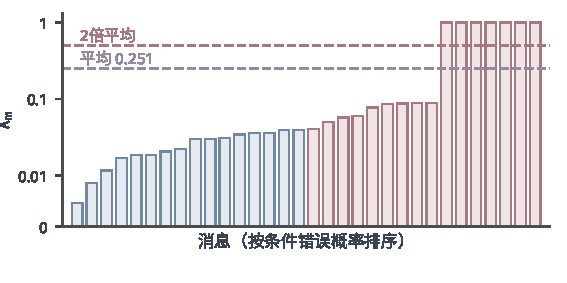
\includegraphics[width=96mm]{figures/07-probability/06-channel-coding/matplotlib/gcc-expurgation/figure.pdf}
 \caption{一个随机高斯码本（种子$5$，$n=12$，$M=32$，$P'=2.4$，$P=3$，$\sigma^2=1$，最近码字判决）中各消息的条件错误概率$\lambda_m$，按大小排序，每条消息用$20000$次噪声模拟估计。超预算的$7$个码字记为$1$。紫色虚线是平均值$0.251$，红色虚线是平均值的两倍；红色柱是删去的一半，保留的消息错误都在$0.04$以下。纵轴在$0.01$以下为线性刻度，以上为对数刻度。}
 \label{fig:gcc-expurgation}
\end{BookInlineFigure}

图~\ref{fig:gcc-expurgation}在一个很短的码上演示这一步。码长只有$12$时，$32$个随机码字中有$7$个超预算，把平均错误抬到$0.251$；删去最差的一半，超预算的码字全部被删掉，剩下的$16$条消息错误都在$0.04$以下。块长增大时，超预算的比例和其他错误都趋于零，删去一半只让码率损失$1/n$。

\paragraph{块长的作用}
证明保证错误趋于零，但没有说多长的块才够。图~\ref{fig:gcc-random-code}用模拟给出一个印象：码率固定为$R=\frac12$，码字取随机方向、长度恰为$\sqrt{nP}$，从而每条码字都恰好用满预算，接收端选与输出最近的码字。$C(P)=\frac12$对应$P/\sigma^2=1$，即$0$分贝。块长从$8$增加到$32$，错误率曲线变陡，在容量对应的信噪比右侧下降得越来越快；但$n=32$时，要把错误率压到$10^{-3}$，信噪比仍需高出约$4$分贝。逼近容量需要长得多的块和高效的译码方法，这是第~\ref{chap:channel-codes}章的话题。

\begin{BookInlineFigure}
 \centering
 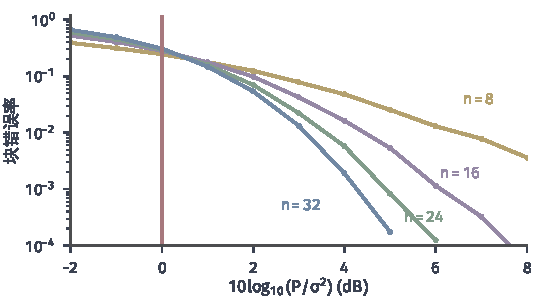
\includegraphics[width=92mm]{figures/07-probability/06-channel-coding/matplotlib/gcc-random-code/figure.pdf}
 \caption{码率$R=\frac12$的随机码在$\sigma^2=1$的高斯信道上的块错误率随信噪比（分贝）的变化，最近码字判决。码字是随机方向上长度为$\sqrt{nP}$的向量。黄、紫、绿、蓝分别对应$n=8,16,24,32$（$M=2^{n/2}$），每点模拟$40000$条消息（种子$11$）。红线是$C(P)=\frac12$对应的$0$分贝。}
 \label{fig:gcc-random-code}
\end{BookInlineFigure}

\paragraph{逆定理}
现在证明第二条：速率超过$C(P)$时，错误不能趋于零。思路与离散信道相同，只是单次互信息的上界换成定理~\ref{thm:gcc-upper}，并且要处理各时刻功率不同的情形。

设$(M,n)$码满足功率约束$P$，消息$W$在$\{1,\dots,M\}$上均匀分布，$X^n=x^n(W)$，$Y^n$是输出。第$i$个时刻在消息上的平均功率记作
\[
 P_i=\mathbb{E}[X_i^2]=\frac1M\sum_{m=1}^{M}x_i(m)^2 .
\]
对$i$求平均，由约束~\eqref{eq:gcc-power}，
\[
 \frac1n\sum_{i=1}^{n}P_i=\frac1M\sum_{m=1}^{M}\frac1n\lVert x^n(m)\rVert_2^2\leq P .
\]

第一步，由第~\ref{chap:information-measures}章的Fano不等式和数据处理不等式，
\[
 \log_2M=H(W)=I(W;Y^n)+H(W\mid Y^n)\leq I(X^n;Y^n)+1+P_{\mathrm{e}}\log_2M .
\]

第二步，上界$I(X^n;Y^n)$。$X^n$只取有限个值，引理~\ref{lem:gcc-output}的证明逐字推广到$n$维：$Y^n$有密度，$h(Y^n)$有限，并且$I(X^n;Y^n)=h(Y^n)-h(Z^n)$。噪声坐标独立，$h(Z^n)=\sum_ih(Z_i)$；由微分熵的链式法则和“条件化不增加熵”，$h(Y^n)\leq\sum_ih(Y_i)$。于是
\[
 I(X^n;Y^n)\leq\sum_{i=1}^{n}\bigl(h(Y_i)-h(Z_i)\bigr)\leq\sum_{i=1}^{n}C(P_i) ,
\]
最后一步对每个时刻用了定理~\ref{thm:gcc-upper}的证明：$\operatorname{Var}(Y_i)\leq P_i+\sigma^2$。

第三步，用凹性合并各时刻。$C(p)=\frac12\log_2(1+p/\sigma^2)$是$p$的凹增函数，由Jensen不等式，
\[
 \sum_{i=1}^{n}C(P_i)\leq n\,C\Bigl(\frac1n\sum_{i=1}^{n}P_i\Bigr)\leq n\,C(P) .
\]
图~\ref{fig:gcc-concavity}说明这一步：把功率在时刻之间不均匀地分配，各时刻上界的平均落在弦上，低于平均功率处的曲线值。

\begin{BookInlineFigure}
 \centering
 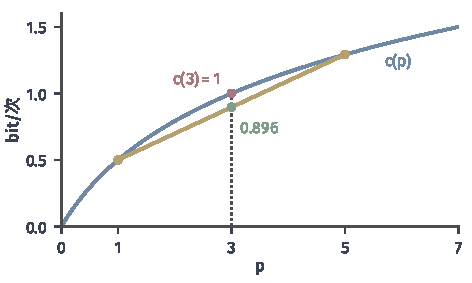
\includegraphics[width=80mm]{figures/07-probability/06-channel-coding/matplotlib/gcc-concavity/figure.pdf}
 \caption{$c(p)=\frac12\log_2(1+p)$（蓝，$\sigma^2=1$）的凹性。一半时刻用功率$1$、一半用$5$，平均功率为$3$；各时刻上界的平均是弦的中点$0.896$（绿），低于$c(3)=1$（红）。}
 \label{fig:gcc-concavity}
\end{BookInlineFigure}

三步合起来，
\begin{equation}
 \log_2M\leq\frac{n\,C(P)+1}{1-P_{\mathrm{e}}} .
 \label{eq:gcc-converse}
\end{equation}
对一列满足约束的码，若$P_{\mathrm{e}}\to0$，两边除以$n$再取上极限，便知码率$\frac1n\log_2M_n$的上极限不超过$C(P)$。定理~\ref{thm:gcc-coding}的第二条得证。

式~\eqref{eq:gcc-converse}也给出错误的下界。以$\sigma^2=1$、$P=3$为例，若码率为$1.2$比特，$\log_2M=1.2n$，整理得
\[
 P_{\mathrm{e}}\geq1-\frac{n+1}{1.2n}\to\frac16 .
\]
块再长，平均错误也不会低于约$16.7\%$。错误概率实际上趋于一，这称为强逆定理，它在这个模型中也成立，但证明需要对信息密度作更细的集中估计，本章不给出证明。

逆定理只用了$\frac1n\sum_iP_i\leq P$，即在消息和时刻上同时平均的功率不超过$P$。所以即使把逐条码字的约束放宽为对消息平均的约束，速率上限仍是$C(P)$；而可达性部分构造的码满足逐条约束。两种约束给出同一个容量。


\section{平行高斯信道}
\label{sec:gcc-parallel}

设发送端同时掌握三条互不干扰的线路，噪声方差分别是$1$、$2$、$5$，但三条线路共用一个功率预算$5$。功率应当平均分给三条线路，全部给最安静的那条，还是另有更好的分法？分法确定以后，三条线路合起来每次能送多少比特？

\paragraph{模型}
设$k$为固定的正整数，$\sigma_1^2,\dots,\sigma_k^2>0$。每次使用信道，发送端送出一个向量$\bm{x}_i=(x_{i,1},\dots,x_{i,k})\in\mathbb{R}^k$，接收端得到
\begin{equation}
 Y_{i,j}=x_{i,j}+Z_{i,j},\qquad j=1,\dots,k,\quad i=1,\dots,n ,
 \label{eq:gcc-parallel}
\end{equation}
其中全部噪声$Z_{i,j}$相互独立，$Z_{i,j}\sim\mathcal{N}(0,\sigma_j^2)$，并且与消息独立。第$j$个分量的噪声方差$\sigma_j^2$不随时刻改变。这样的信道称为\term{平行高斯信道}（parallel Gaussian channel）。

满足功率约束$P$的$(M,n)$码要求每条码字在所有时刻与所有分量上的总能量不超过$nP$：
\begin{equation}
 \sum_{i=1}^{n}\sum_{j=1}^{k}x_{i,j}(m)^2\leq nP,\qquad m=1,\dots,M .
 \label{eq:gcc-parallel-power}
\end{equation}
码率仍是$\frac1n\log_2M$，单位是比特每次向量使用。图~\ref{fig:gcc-parallel-model}画出$k=3$的情形。

\begin{BookInlineFigure}
 \centering
 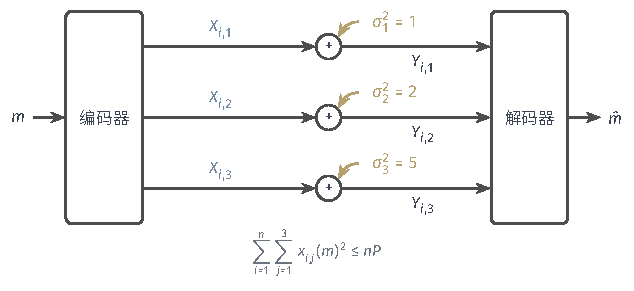
\includegraphics[width=107mm]{figures/07-probability/06-channel-coding/tikz/gcc-parallel-model/figure.pdf}
 \caption{$k=3$的平行高斯信道。第$i$次使用时，向量输入的三个分量（蓝）分别加上方差为$1,2,5$的独立噪声（黄）；三个分量和全部$n$次使用共享同一个能量预算$nP$。}
 \label{fig:gcc-parallel-model}
\end{BookInlineFigure}

\paragraph{单次使用的上界}
与标量情形一样，先在单次使用上优化。设随机输入向量$\bm{X}$的分量为$X_1,\dots,X_k$，平均能量$\mathbb{E}\lVert\bm{X}\rVert_2^2\leq P$，它与噪声向量$\bm{Z}$独立，输出$\bm{Y}=\bm{X}+\bm{Z}$。记第$j$个分量的功率为$P_j=\mathbb{E}[X_j^2]$，它们的和不超过$P$。

引理~\ref{lem:gcc-output}的证明对向量逐字成立：$\bm{Y}$有密度，$h(\bm{Y})$有限，并且
\[
 I(\bm{X};\bm{Y})=h(\bm{Y})-h(\bm{Z}) .
\]
噪声分量独立，所以$h(\bm{Z})$等于各$h(Z_j)$之和。由第~\ref{chap:information-measures}章熵的链式法则和条件化不增加熵，联合微分熵不超过各分量微分熵之和：
\[
 h(\bm{Y})\leq\sum_{j=1}^{k}h(Y_j) .
\]
每个分量的方差不超过$P_j+\sigma_j^2$，对每个分量用引理~\ref{lem:gcc-max-entropy}，得到
\begin{equation}
 I(\bm{X};\bm{Y})\leq\sum_{j=1}^{k}\bigl(h(Y_j)-h(Z_j)\bigr)\leq\sum_{j=1}^{k}\frac12\log_2\Bigl(1+\frac{P_j}{\sigma_j^2}\Bigr) .
 \label{eq:gcc-parallel-upper}
\end{equation}

这个上界可以取到：让各分量独立，$X_j\sim\mathcal{N}(0,P_j)$。此时各$Y_j$独立，次可加性取等号；每个$Y_j$是方差$P_j+\sigma_j^2$的高斯变量，熵上界也取等号。于是单次使用的问题化为一个只关于功率分配$(P_1,\dots,P_k)$的有限维问题。

\subsection{注水分配}
\label{sec:gcc-waterfilling}

要求解的是
\begin{equation}
 \max_{P_1,\dots,P_k}\ \sum_{j=1}^{k}\frac12\log_2\Bigl(1+\frac{P_j}{\sigma_j^2}\Bigr)
 \quad\text{s.t.}\quad P_j\geq0,\quad\sum_{j=1}^{k}P_j\leq P .
 \label{eq:gcc-allocation}
\end{equation}

\paragraph{边际收益}
先看每个分量多分一点功率能多得多少。第$j$项对$P_j$的导数是
\[
 \frac{\partial}{\partial P_j}\,\frac12\log_2\Bigl(1+\frac{P_j}{\sigma_j^2}\Bigr)=\frac{1}{2\ln2}\cdot\frac{1}{\sigma_j^2+P_j} .
\]
它随$P_j$增大而减小，并且在$P_j=0$处等于$1/(2\ln2\,\sigma_j^2)$：噪声越小的分量，第一份功率越值钱。于是分配应当从最安静的分量开始；它的边际收益随投入下降，降到与次安静分量的起始值相等时，再同时投入两者，使两者的边际收益保持相等，依此类推。最优时，所有分到功率的分量边际收益相同，没分到功率的分量起始收益不高于这个公共值。

\paragraph{乘子条件}
把上面的直观写成严格的最优性条件。目标函数是凹函数，约束是线性的，并且$P>0$时$P_j=P/(2k)$严格满足所有不等式约束。由卷五的凸优化理论，KKT条件对最优解既必要又充分，可参考\BookChapterRef{chap:constrained-optimality}{卷五第17章“约束问题的最优性”}。引入预算约束的乘子$\mu\geq0$与非负约束的乘子$\eta_j\geq0$，KKT条件是
\[
 \frac{1}{2\ln2}\cdot\frac{1}{\sigma_j^2+P_j}=\mu-\eta_j,\qquad \eta_jP_j=0,\qquad \mu\Bigl(P-\sum_{j}P_j\Bigr)=0 .
\]

目标函数关于每个$P_j$严格递增，预算不会留有剩余，所以$\sum_jP_j=P$且$\mu>0$。记$\nu=1/(2\ln2\,\mu)$。若$P_j>0$，则$\eta_j=0$，由第一式得$\sigma_j^2+P_j=\nu$；若$P_j=0$，则$\eta_j\geq0$，由第一式得$1/\sigma_j^2\leq1/\nu$，即$\sigma_j^2\geq\nu$。两种情形合并为$P_j=\max\{\nu-\sigma_j^2,0\}$。

\begin{theorem}[注水分配]
\label{thm:gcc-waterfilling}
设$P>0$，$\sigma_j^2>0$。问题~\eqref{eq:gcc-allocation}的唯一最优解是
\begin{equation}
 P_j=(\nu-\sigma_j^2)^{+},\qquad j=1,\dots,k,
 \label{eq:gcc-waterfilling}
\end{equation}
其中$(t)^{+}=\max\{t,0\}$，水位$\nu$是方程$\sum_{j=1}^{k}(\nu-\sigma_j^2)^{+}=P$的唯一解。平行高斯信道的信息容量是
\begin{equation}
 C(P)=\sum_{j=1}^{k}\frac12\log_2\Bigl(1+\frac{(\nu-\sigma_j^2)^{+}}{\sigma_j^2}\Bigr)
 =\sum_{j:\,\sigma_j^2<\nu}\frac12\log_2\frac{\nu}{\sigma_j^2} .
 \label{eq:gcc-parallel-capacity}
\end{equation}
\end{theorem}

\begin{proof}
函数$\nu\mapsto\sum_j(\nu-\sigma_j^2)^{+}$连续、不减，在$\nu\leq\min_j\sigma_j^2$时为零，在$\nu>\min_j\sigma_j^2$时严格递增且趋于无穷，所以方程有唯一解$\nu>\min_j\sigma_j^2$。由此定义的$P_j$非负、总和为$P$；取$\mu=1/(2\ln2\,\nu)$，$P_j>0$时取$\eta_j=0$，$P_j=0$时取$\eta_j=\mu-1/(2\ln2\,\sigma_j^2)\geq0$，KKT条件全部满足，所以它是最优解。目标函数是各分量严格凹函数之和，因而在可行集上严格凹，最优解唯一。代入目标函数，活跃分量上$1+P_j/\sigma_j^2=\nu/\sigma_j^2$，即得式~\eqref{eq:gcc-parallel-capacity}。
\end{proof}

式~\eqref{eq:gcc-waterfilling}称为\term{注水}（water-filling）分配。把第$j$个分量画成底部高度为$\sigma_j^2$的一格容器，往这排容器里倒总量为$P$的水，水面在各格中齐平，高度就是$\nu$；每格的水深就是分给它的功率。底部高于水面的格子一滴水也没有。类比的对应是：底部高度对应噪声方差，水的总量对应预算，水面齐平对应边际收益相等。类比只描述分配规则，水深与容量的关系仍要回到对数公式。

\paragraph{例：三条线路}
回到本节开头的问题：$\sigma^2=(1,2,5)$，$P=5$。把噪声方差从小到大排列，先假设只有最安静的$a$个分量活跃，由$\sum_{j\leq a}(\nu-\sigma_j^2)=P$解出
\[
 \nu_a=\frac{1}{a}\Bigl(P+\sum_{j=1}^{a}\sigma_j^2\Bigr),
\]
再检查它是否高于第$a$个、不高于第$a+1$个噪声方差。$a=3$时$\nu_3=(5+8)/3=4.33$，低于$\sigma_3^2=5$，第三个分量分不到功率，假设不成立。$a=2$时$\nu_2=(5+3)/2=4$，高于$\sigma_2^2=2$，不高于$\sigma_3^2=5$，成立。于是
\[
 \nu=4,\qquad P_1=3,\quad P_2=2,\quad P_3=0 .
\]
代入式~\eqref{eq:gcc-parallel-capacity}，容量是
\[
 C=\frac12\log_2\frac41+\frac12\log_2\frac42=1+\frac12=1.5\ \text{比特每次向量使用}.
\]

作为对照，平均分配$P_j=5/3$得到
\[
 \frac12\log_2\Bigl(1+\frac53\Bigr)+\frac12\log_2\Bigl(1+\frac56\Bigr)+\frac12\log_2\Bigl(1+\frac13\Bigr)=1.352 ;
\]
全部给第一个分量得到$\frac12\log_2 6=1.292$。平均分配把三分之一的预算放在噪声最大的分量上，那里每单位功率换来的信息最少；全部给第一个分量则让它的边际收益降到$1/(2\ln2\cdot6)$，低于第二个分量起始的$1/(2\ln2\cdot2)$。图~\ref{fig:gcc-waterfilling}(a)画出注水的结果。

\begin{BookInlineFigure}
 \centering
 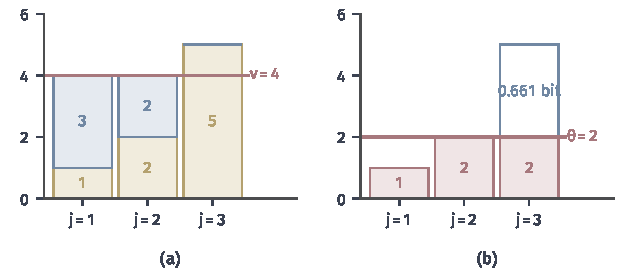
\includegraphics[width=106mm]{figures/07-probability/06-channel-coding/matplotlib/gcc-waterfilling/figure.pdf}
 \caption{两种“注水”的对照，三个分量的方差都是$(1,2,5)$。(a)平行高斯信道的功率分配，总功率$5$：黄色是噪声方差构成的底，蓝色是分到的功率，红线是水位$\nu=4$，功率为$(3,2,0)$。(b)第~\ref{chap:rate-distortion}章独立高斯分量的反注水，总失真$5$：红色是各分量的失真$\min\{\theta,\sigma_j^2\}$，红线是$\theta=2$，蓝框中高出$\theta$的部分需要描述，码率为$(0,0,0.661)$比特。}
 \label{fig:gcc-waterfilling}
\end{BookInlineFigure}

\paragraph{预算增加时}
水位随预算连续上升，分量按噪声从小到大依次加入。例中水位到达$2$时第二个分量开始分到功率，此时$P=\nu-1=1$；水位到达$5$时第三个分量加入，此时$P=(5-1)+(5-2)=7$。所以
\[
 P\leq1:\ \text{只用分量}1;\qquad 1<P\leq7:\ \text{用分量}1,2;\qquad P>7:\ \text{三个都用}.
\]
在每一段内，活跃分量的功率随$P$线性增长，斜率都是$1/a$，$a$是活跃分量数。图~\ref{fig:gcc-waterfill-path}(a)画出三条分配曲线，(b)比较三种分配方式的容量。

\begin{BookInlineFigure}
 \centering
 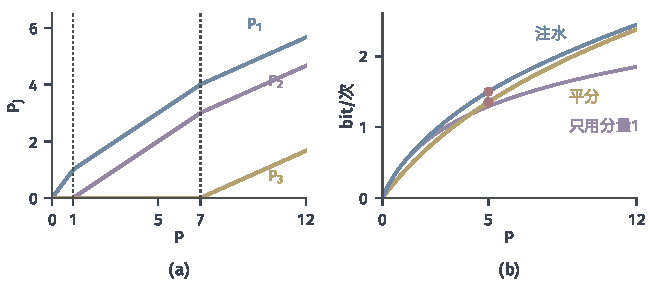
\includegraphics[width=110mm]{figures/07-probability/06-channel-coding/matplotlib/gcc-waterfill-path/figure.pdf}
 \caption{噪声方差为$(1,2,5)$时随总功率$P$的变化。(a)注水分配给三个分量的功率$P_1$（蓝）、$P_2$（紫）、$P_3$（黄），点线标出分量加入的位置$P=1$与$P=7$。(b)容量：注水分配（蓝）、平均分配（黄）、全部给分量$1$（紫）；红点是$P=5$时的$1.5$与$1.352$。}
 \label{fig:gcc-waterfill-path}
\end{BookInlineFigure}

乘子还有一层含义。由第~\ref{chap:discrete-channel-capacity}章成本约束下乘子的解释，$\mu$是预算的边际价值：总预算增加一个小量$\delta$，容量约增加$\mu\delta$。例中$\nu=4$，
\[
 \mu=\frac{1}{2\ln2\cdot4}=0.180\ \text{比特每单位功率}.
\]
直接验证：新增的功率平均分给两个活跃分量，每个水深增加$\delta/2$，每个分量的边际收益都是$1/(2\ln2\cdot4)$，容量增加约
\[
 2\cdot\frac{1}{2\ln2\cdot4}\cdot\frac{\delta}{2}=\mu\delta .
\]
第三个分量的起始边际收益是$1/(2\ln2\cdot5)=0.144$，低于$\mu=0.180$，这正是KKT条件中$\eta_3=\mu-0.144\geq0$的含义：把功率挪一点给它，只会得不偿失。

\paragraph{与反注水的对照}
第~\ref{chap:rate-distortion}章为独立高斯信源分配码率时也出现了一个“水位”，称为反注水：各分量的失真取$D_j=\min\{\theta,\sigma_j^2\}$，方差不超过$\theta$的分量不必描述。两种分配形式相似，分配的对象和方向却相反。图~\ref{fig:gcc-waterfilling}把它们并排画出，表~\ref{tab:gcc-water-vs-reverse}列出对应关系。

\begin{BookInlineTable}
 \centering
 \caption{注水与反注水的对照}
 \label{tab:gcc-water-vs-reverse}
 \begin{tabular}{lll}
  \toprule
   & 注水（信道） & 反注水（信源） \\
  \midrule
  分配的量 & 发送功率$P_j$ & 允许的失真$D_j$ \\
  分配规则 & $P_j=(\nu-\sigma_j^2)^{+}$ & $D_j=\min\{\theta,\sigma_j^2\}$ \\
  $\sigma_j^2$的含义 & 噪声方差 & 信源方差 \\
  被舍弃的分量 & 噪声高于水位 & 方差低于水位 \\
  目标 & 最大化容量 & 最小化码率 \\
  \bottomrule
 \end{tabular}
\end{BookInlineTable}

信道一侧，水倒在噪声上面，噪声越小的分量越先得到功率，因为同样的功率在那里换来更多的可区分性。信源一侧，水位以下是允许的失真，方差越大的分量越需要码率，方差小于水位的分量直接用均值重构即可。两种问题都把总资源按边际收益相等的原则分配，只是一个分配的是用来传送的资源，一个分配的是允许损失的量。

\subsection{并行传输的计量}
\label{sec:gcc-parallel-accounting}

式~\eqref{eq:gcc-parallel-capacity}是单次向量使用上的信息容量。它的单位、它与标量公式的关系，以及它是否也是块码的速率极限，需要分别说明。

\paragraph{一次向量使用}
一次使用同时占用$k$个实分量，容量计的是这$k$个分量合起来送出的比特数。例中$C=1.5$比特每次向量使用，折合每个实分量$0.5$比特；这两个数不能与单个实分量的公式~\eqref{eq:gcc-capacity}直接比较。比如把全部功率$5$放在一条噪声方差为$1$的标量信道上，得到$\frac12\log_2 6=1.292$比特每次使用，它比$1.5$小，比$0.5$大：前者比的是同一预算下“一条线路”与“三条线路”的总量，后者把三条线路的总量摊到了每条线路上。比较时要先说清楚：资源是什么（总功率还是每条线路的功率），计量单位是什么（每次向量使用还是每个实分量）。

复值信道就是$k=2$且两分量噪声相同的平行信道。两个噪声方差都是$\sigma^2/2$，注水的水位是$\nu=\sigma^2/2+P/2$，两分量平分功率，容量是
\[
 2\cdot\frac12\log_2\frac{\sigma^2/2+P/2}{\sigma^2/2}=\log_2\Bigl(1+\frac{P}{\sigma^2}\Bigr)\ \text{比特每次复值使用},
\]
这回答了第~\ref{sec:gcc-optimal-input}小节留下的问题：平分不是约定，而是最优分配。

\paragraph{可达性}
单次使用的容量能否被块码达到，回答与标量情形相同。

\begin{theorem}[平行信道的编码定理]
\label{thm:gcc-parallel-coding}
设分量数$k$固定，$P>0$，信道由式~\eqref{eq:gcc-parallel}给出，码满足约束~\eqref{eq:gcc-parallel-power}。低于式~\eqref{eq:gcc-parallel-capacity}中$C(P)$的速率都可达，且最大错误概率可以趋于零；平均错误概率趋于零的码列，其码率的上极限不超过$C(P)$。
\end{theorem}

可达性可以直接由标量结果拼出来。设$R<C(P)$，$(P_1,\dots,P_k)$是注水分配，活跃分量的集合记作$J$。因为$R<\sum_{j\in J}\frac12\log_2(1+P_j/\sigma_j^2)$，可以把$R$拆成$R=\sum_{j\in J}R_j$，使每个$R_j$严格小于第$j$个分量的标量容量。对每个$j\in J$，由定理~\ref{thm:gcc-coding}，存在第$j$个分量上满足功率约束$P_j$、码率至少$R_j$、最大错误概率$\lambda^{(j)}_{\max}\to0$的码；不活跃的分量始终发送零。

把各分量的消息组成向量$m=(m_j)_{j\in J}$，消息总数是各分量消息数之积，至少为$2^{nR}$。每条组合码字的总能量不超过$n\sum_jP_j=nP$。接收端在每个分量上独立解码，只要有一个分量判错，整条消息就判错；由并集界，最大错误概率不超过$\sum_{j\in J}\lambda^{(j)}_{\max}\to0$。

也可以不拆分，把第~\ref{sec:gcc-coding}小节的证明中的“字母”换成$k$维向量：码字在每个时刻独立地抽取$\mathcal{N}(0,P_j')$的各分量，信息密度是各分量信息密度之和，三类错误的估计逐字成立，只是能量和信息密度的平均对时刻和分量同时进行。这种做法说明向量信息密度的集中同样可以控制整组分量的联合判决。

\paragraph{逆定理}
逆向的论证与标量情形相同，只多一层对分量的求和。记$P_{i,j}=\frac1M\sum_mx_{i,j}(m)^2$为第$i$个时刻第$j$个分量在消息上的平均功率。Fano不等式和数据处理之后，与第~\ref{sec:gcc-coding}小节的第二步相同，得到
\[
 I(X^n;Y^n)\leq\sum_{i=1}^{n}F(P_{i,1},\dots,P_{i,k}),\qquad
 F(p_1,\dots,p_k)=\sum_{j=1}^{k}\frac12\log_2\Bigl(1+\frac{p_j}{\sigma_j^2}\Bigr) .
\]
$F$是凹函数，由Jensen不等式，$\sum_iF(\bm{p}_i)\leq nF(\bar{\bm{p}})$，其中$\bar{\bm{p}}$是各时刻分配向量的平均。约束~\eqref{eq:gcc-parallel-power}保证$\bar{\bm{p}}$的分量之和不超过$P$，所以$F(\bar{\bm{p}})\leq C(P)$。其余步骤与式~\eqref{eq:gcc-converse}相同。

论证依赖两个条件：分量数$k$固定，不随块长增长；噪声在时间上独立，且各分量的方差不随时刻改变。若$k$随$n$增长，或者噪声方差随时刻变化，就需要重新处理这里的大数律和单次上界。


\section{相关高斯噪声}
\label{sec:gcc-correlated}

平行信道假设各分量的噪声互相独立。两条并排的线路常常受到同一个干扰源的影响，噪声会相关。设两条线路的噪声方差都是$2$，协方差是$1$，即
\[
 \bm{Z}\sim\mathcal{N}(\bm{0},\bm{\Sigma}),\qquad \bm{\Sigma}=\begin{bmatrix}2&1\\1&2\end{bmatrix},
\]
总功率预算为$P=2$。这时各分量不能单独处理，注水规则还能用吗？功率应当分给哪个方向？

\paragraph{模型}
设$\bm{\Sigma}$是$k\times k$实对称正定矩阵。每次使用时输入$\bm{x}_i\in\mathbb{R}^k$，输出
\begin{equation}
 \bm{Y}_i=\bm{x}_i+\bm{Z}_i,\qquad \bm{Z}_1,\dots,\bm{Z}_n\ \text{独立同分布},\ \bm{Z}_i\sim\mathcal{N}(\bm{0},\bm{\Sigma}),
 \label{eq:gcc-correlated}
\end{equation}
噪声与消息独立。码字满足欧氏总能量约束$\sum_{i=1}^{n}\lVert\bm{x}_i(m)\rVert_2^2\leq nP$。同一时刻各分量的噪声可以相关，不同时刻之间仍然独立。

\paragraph{正交变换}
由谱分解（\BookChapterRef{chap:eigen-spectral-decomposition}{卷二第6章“谱分解”}），$\bm{\Sigma}=\bm{U}\bm{\Lambda}\bm{U}^{\top}$，其中$\bm{U}$是正交矩阵，列向量$\bm{u}_1,\dots,\bm{u}_k$是$\bm{\Sigma}$的单位特征向量，$\bm{\Lambda}$是以特征值$\lambda_1,\dots,\lambda_k$为对角元的对角阵，正定性保证每个$\lambda_j>0$。在特征向量的坐标下看噪声：
\[
 \tilde{\bm{Z}}=\bm{U}^{\top}\bm{Z}\sim\mathcal{N}\bigl(\bm{0},\bm{U}^{\top}\bm{\Sigma}\bm{U}\bigr)=\mathcal{N}(\bm{0},\bm{\Lambda}) .
\]
$\tilde{\bm{Z}}$的协方差矩阵是对角阵，各分量不相关；它们又是联合高斯的，由第~\ref{chap:multivariate-distributions}章，不相关的联合高斯分量相互独立。所以在这组坐标下，噪声变成了方差为$\lambda_1,\dots,\lambda_k$的独立分量。

同一组坐标也保持功率预算：$\bm{U}$是正交矩阵，对任意$\bm{x}\in\mathbb{R}^k$，
\[
 \lVert\bm{U}^{\top}\bm{x}\rVert_2=\lVert\bm{x}\rVert_2 .
\]
噪声变得独立、预算形式不变，这两点合起来说明相关噪声信道与平行信道等价。

\begin{lemma}[正交坐标下的等价]
\label{lem:gcc-rotation}
对式~\eqref{eq:gcc-correlated}的信道，记噪声方差为$\lambda_1,\dots,\lambda_k$的平行信道为$\tilde{\mathcal{C}}$。满足功率约束$P$的$(M,n)$码在两个信道之间可以一一对应，对应的码满足同样的约束，并且每条消息的条件错误概率相同。
\end{lemma}

\begin{proof}
设$(\tilde{f},\tilde{g})$是$\tilde{\mathcal{C}}$上的码，消息$m$的码字由$n$个向量$\tilde{\bm{x}}_i(m)$组成，$i=1,\dots,n$。在相关噪声信道上，令编码器发送$\bm{x}_i(m)=\bm{U}\tilde{\bm{x}}_i(m)$，解码器先把每个输出向量乘以$\bm{U}^{\top}$，再用$\tilde{g}$判决。能量逐时刻保持，所以约束成立。发送消息$m$时，
\[
 \bm{U}^{\top}\bm{Y}_i=\tilde{\bm{x}}_i(m)+\bm{U}^{\top}\bm{Z}_i ,
\]
$\bm{U}^{\top}\bm{Z}_1,\dots,\bm{U}^{\top}\bm{Z}_n$独立同分布于$\mathcal{N}(\bm{0},\bm{\Lambda})$，所以$\tilde{g}$看到的输入与在$\tilde{\mathcal{C}}$上看到的分布完全相同，条件错误概率相同。反方向把$\bm{U}$与$\bm{U}^{\top}$对调即可。
\end{proof}

图~\ref{fig:gcc-rotation-equivalence}画出这个对应：发送端和接收端各乘一个正交矩阵，中间的相关噪声信道在外面看来就是平行信道。

\begin{BookInlineFigure}
 \centering
 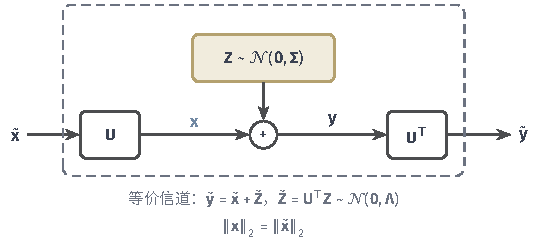
\includegraphics[width=90mm]{figures/07-probability/06-channel-coding/tikz/gcc-rotation-equivalence/figure.pdf}
 \caption{相关噪声信道与平行信道的等价。发送端把$\tilde{\bm{x}}$变成$\bm{x}=\bm{U}\tilde{\bm{x}}$，信道加上噪声$\bm{Z}\sim\mathcal{N}(\bm{0},\bm{\Sigma})$（黄框），接收端乘以$\bm{U}^{\top}$。虚线框整体是噪声方差为$\lambda_1,\dots,\lambda_k$的平行信道，正交变换保持欧氏长度。}
 \label{fig:gcc-rotation-equivalence}
\end{BookInlineFigure}

由引理~\ref{lem:gcc-rotation}和定理~\ref{thm:gcc-parallel-coding}，相关噪声信道的容量就是对特征值$\lambda_1,\dots,\lambda_k$注水得到的值。最优输入也可以写回原坐标。

\begin{theorem}[相关高斯噪声信道的容量]
\label{thm:gcc-correlated}
设$\bm{\Sigma}$正定，特征分解为$\bm{U}\bm{\Lambda}\bm{U}^{\top}$，$P>0$。式~\eqref{eq:gcc-correlated}的信道在功率约束$P$下的容量是
\begin{equation}
 C(P)=\sum_{j=1}^{k}\frac12\log_2\Bigl(1+\frac{(\nu-\lambda_j)^{+}}{\lambda_j}\Bigr),\qquad \sum_{j=1}^{k}(\nu-\lambda_j)^{+}=P .
 \label{eq:gcc-correlated-capacity}
\end{equation}
单次使用的最优输入是$\bm{X}\sim\mathcal{N}(\bm{0},\bm{K}^{\star})$，其中
\begin{equation}
 \bm{K}^{\star}=\bm{U}\operatorname{diag}\bigl((\nu-\lambda_1)^{+},\dots,(\nu-\lambda_k)^{+}\bigr)\bm{U}^{\top} ,
 \label{eq:gcc-optimal-covariance}
\end{equation}
并且
\begin{equation}
 C(P)=\max_{\bm{K}\succeq\bm{0},\ \operatorname{tr}\bm{K}\leq P}\ \frac12\log_2\frac{\det(\bm{\Sigma}+\bm{K})}{\det\bm{\Sigma}} .
 \label{eq:gcc-logdet}
\end{equation}
\end{theorem}

\begin{proof}
式~\eqref{eq:gcc-correlated-capacity}由引理~\ref{lem:gcc-rotation}与定理~\ref{thm:gcc-parallel-coding}、定理~\ref{thm:gcc-waterfilling}得到。再看式~\eqref{eq:gcc-logdet}。$k$维高斯向量$\mathcal{N}(\bm{0},\bm{A})$的微分熵是$\frac12\log_2\bigl((2\pi\mathrm{e})^k\det\bm{A}\bigr)$。对输入$\bm{X}\sim\mathcal{N}(\bm{0},\bm{K})$，输出$\bm{Y}\sim\mathcal{N}(\bm{0},\bm{\Sigma}+\bm{K})$，由$I(\bm{X};\bm{Y})=h(\bm{Y})-h(\bm{Z})$，
\[
 I(\bm{X};\bm{Y})=\frac12\log_2\frac{\det(\bm{\Sigma}+\bm{K})}{\det\bm{\Sigma}} .
\]
输入的平均能量是协方差矩阵的迹，可行的$\bm{K}$满足$\operatorname{tr}\bm{K}\leq P$。互信息在两端的可逆线性变换下不变（第~\ref{chap:information-measures}章），所以
\[
 I(\bm{X};\bm{Y})=I(\bm{U}^{\top}\bm{X};\bm{U}^{\top}\bm{Y}) ,
\]
右端是平行信道$\tilde{\mathcal{C}}$上一个满足预算的输入的互信息，由式~\eqref{eq:gcc-parallel-upper}和定理~\ref{thm:gcc-waterfilling}不超过$C(P)$。另一方面，$\bm{K}=\bm{K}^{\star}$对应平行信道上的独立高斯注水输入，取到$C(P)$。
\end{proof}

\paragraph{例：两条相关的线路}
回到本节开头的例子。$\bm{\Sigma}$的特征值和单位特征向量是
\[
 \lambda_1=1,\ \bm{u}_1=\tfrac{1}{\sqrt2}(1,-1)^{\top};\qquad \lambda_2=3,\ \bm{u}_2=\tfrac{1}{\sqrt2}(1,1)^{\top} .
\]
沿$\bm{u}_2$方向，两条线路的噪声同向，叠加得大；沿$\bm{u}_1$方向，共同的干扰在两条线路的差中抵消，只剩方差$1$。

对$(\lambda_1,\lambda_2)=(1,3)$注水，预算$P=2$。先试两个分量都活跃：$\nu=(2+1+3)/2=3$，恰好等于$\lambda_2$，第二个分量的功率是$0$。所以
\[
 \nu=3,\qquad P_1=2,\quad P_2=0,\qquad C=\frac12\log_2 3=0.792\ \text{比特每次使用}.
\]
最优输入是$\bm{X}=X_1\bm{u}_1$，$X_1\sim\mathcal{N}(0,2)$：两条线路发送大小相同、符号相反的信号，每条线路的平均功率是$1$。接收端看两条线路的差，共同干扰被抵消。

对照两种做法。若忽略相关性，让两条线路独立地各用功率$1$，即$\bm{K}=\bm{I}$，由式~\eqref{eq:gcc-logdet}，
\[
 \frac12\log_2\frac{\det(\bm{\Sigma}+\bm{I})}{\det\bm{\Sigma}}=\frac12\log_2\frac{8}{3}=0.708 .
\]
若两条线路的噪声方差仍是$2$，但相互独立，平均分配功率得到$2\cdot\frac12\log_2(1+\frac12)=0.585$。同样的边缘方差，相关的噪声反而让容量更大：相关性造出了一个噪声较小的方向，前提是发送端知道这个方向并把功率放在那里。图~\ref{fig:gcc-correlated-noise}画出原坐标和旋转后的坐标。

\begin{BookInlineFigure}
 \centering
 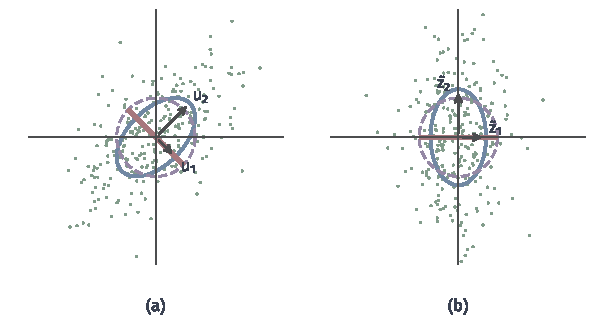
\includegraphics[width=104mm]{figures/07-probability/06-channel-coding/matplotlib/gcc-correlated-noise/figure.pdf}
 \caption{协方差为$\bm{\Sigma}=\bigl[\begin{smallmatrix}2&1\\1&2\end{smallmatrix}\bigr]$的噪声。绿点是$250$个噪声样本（种子$3$），蓝色椭圆是$\bm{z}^{\top}\bm{\Sigma}^{-1}\bm{z}=1$，黑色箭头是$\sqrt{\lambda_j}\bm{u}_j$，紫色虚线圆的半径是$\sqrt{P}=\sqrt2$，红色线段是最优输入沿$\bm{u}_1$方向的$\pm$一个标准差。(a)原坐标。(b)乘以$\bm{U}^{\top}$后的坐标，噪声分量独立，方差为$1$与$3$。}
 \label{fig:gcc-correlated-noise}
\end{BookInlineFigure}

\paragraph{白化}
另一种常见的处理是先把噪声变成单位协方差。接收端把输出乘以对称矩阵$\bm{\Sigma}^{-1/2}$，它与$\bm{\Sigma}$有相同的特征向量，特征值为$\lambda_j^{-1/2}$。这一操作称为白化：
\[
 \bar{\bm{Y}}=\bm{\Sigma}^{-1/2}\bm{Y}=\bm{\Sigma}^{-1/2}\bm{X}+\bm{N},\qquad \bm{N}=\bm{\Sigma}^{-1/2}\bm{Z}\sim\mathcal{N}(\bm{0},\bm{I}) .
\]
接收端的可逆变换可以随时撤销，不改变容量。但白化以后，信道的“输入”变成了$\bar{\bm{X}}=\bm{\Sigma}^{-1/2}\bm{X}$。若把$\bar{\bm{X}}$当作新的输入，信道是$\bar{\bm{Y}}=\bar{\bm{X}}+\bm{N}$，噪声是白的，预算却要跟着变：
\[
 \lVert\bm{X}\rVert_2^2=\lVert\bm{\Sigma}^{1/2}\bar{\bm{X}}\rVert_2^2=\bar{\bm{X}}^{\top}\bm{\Sigma}\bar{\bm{X}} .
\]
于是约束成为带权的预算
\begin{equation}
 \sum_{i=1}^{n}\bar{\bm{x}}_i^{\top}\bm{\Sigma}\bar{\bm{x}}_i\leq nP .
 \label{eq:gcc-weighted-budget}
\end{equation}
沿$\bm{u}_j$方向，$\bar{\bm{x}}$每单位平方长度要花$\lambda_j$单位的实际功率。

若忽略这一点，把白化后的问题当作单位噪声、欧氏预算的普通平行信道，注水会把功率平分，得到错误的答案。例中两个分量噪声都是$1$，平分预算$2$，得到
\[
 2\cdot\frac12\log_2(1+1)=1\ \text{比特},
\]
高于真正的容量$0.792$。多出来的部分来自一个不存在的便宜方向：沿$\bm{u}_2$放置的$\bar{\bm{x}}$实际要付三倍的功率。图~\ref{fig:gcc-whitening}画出白化后的坐标：噪声云变圆，真正的预算是紫色椭圆，错误的预算是黄色虚线圆。

\begin{BookInlineFigure}
 \centering
 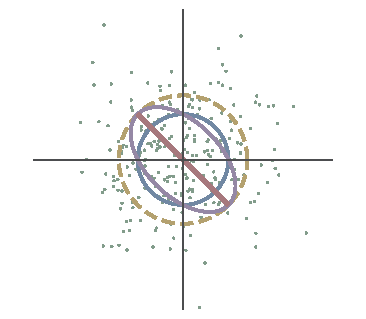
\includegraphics[width=62mm]{figures/07-probability/06-channel-coding/matplotlib/gcc-whitening/figure.pdf}
 \caption{白化后的坐标（与图~\ref{fig:gcc-correlated-noise}同一组噪声样本，绿点）。蓝圆是单位噪声的等高线；紫色椭圆是真正的预算$\bar{\bm{x}}^{\top}\bm{\Sigma}\bar{\bm{x}}\leq P$，沿$\bm{u}_1$的半轴为$\sqrt2$，沿$\bm{u}_2$的半轴为$\sqrt{2/3}$；黄色虚线圆是错误的预算$\lVert\bar{\bm{x}}\rVert_2^2\leq P$。红色线段是最优输入方向。}
 \label{fig:gcc-whitening}
\end{BookInlineFigure}

正确的做法有两种，结果相同。其一，保留原来的输入$\bm{X}$，把白化后的信道写成带增益的形式$\bar{\bm{Y}}=\bm{G}\bm{X}+\bm{N}$，$\bm{G}=\bm{\Sigma}^{-1/2}$。在特征向量坐标下，第$j$个分量是
\[
 \tilde{Y}_j=\lambda_j^{-1/2}\tilde{X}_j+N_j ,
\]
增益为$\lambda_j^{-1/2}$。两边乘以$\lambda_j^{1/2}$，得到$\tilde{X}_j$加上方差$\lambda_j$的噪声，回到对$\lambda_j$注水。其二，保留带权预算，把沿$\bm{u}_j$方向的白化输入功率记为$\bar{p}_j$，它的实际成本是$\lambda_j\bar{p}_j$，容量贡献是$\frac12\log_2(1+\bar{p}_j)$；令$P_j=\lambda_j\bar{p}_j$，问题又变成$\sum_j\frac12\log_2(1+P_j/\lambda_j)$在$\sum_jP_j\leq P$下的最大化。

\paragraph{一般的可逆变换}
上面的现象对任何可逆变换都成立。接收端的可逆变换不改变互信息，也不改变容量。发送端若用可逆矩阵$\bm{A}$换元，$\bm{X}=\bm{A}\bar{\bm{X}}$，预算中的$\lVert\bm{X}\rVert_2^2$就变成以$\bm{A}^{\top}\bm{A}$为矩阵的二次型；只有$\bm{A}$是正交矩阵时，$\bm{A}^{\top}\bm{A}=\bm{I}$，欧氏预算才保持原样。容量是“信道加约束”这一整体的性质，变换信道时必须同时变换约束。

同样的办法处理带增益矩阵的信道$\bm{Y}=\bm{H}\bm{X}+\bm{N}$，$\bm{H}$可逆，$\bm{N}\sim\mathcal{N}(\bm{0},\bm{I})$。由奇异值分解$\bm{H}=\bm{V}\bm{S}\bm{U}^{\top}$，发送端用$\bm{U}$、接收端用$\bm{V}^{\top}$，两者都是正交矩阵，信道化为增益为奇异值$s_j$的平行分量；每个分量除以增益后，等价于噪声方差为$1/s_j^2$的平行信道，再对$1/s_j^2$注水。

\paragraph{正定的作用}
定理要求$\bm{\Sigma}$正定。若$\bm{\Sigma}$有一个特征值为零，相应方向上没有噪声：沿这个方向发送任意实数，接收端在这个方向上的投影就是它本身，于是不同的实数都能被区分，容量为无穷。特征值很小但为正时，容量有限；这个方向的水底最低，注水时它最先分到功率。


\section{本章小结}
\label{sec:gcc-summary}

本章回答了章首的问题：独立高斯噪声下，每次使用在功率预算$P$内最多能可靠送出多少比特。答案由三层论证组成。

第一层是上界。输入二阶矩有限、噪声独立且方差为正时，输出有密度，互信息等于输出熵减去噪声熵；输出方差不超过$P+\sigma^2$，固定方差时高斯分布的熵最大，于是单次互信息不超过$\frac12\log_2(1+P/\sigma^2)$。去掉任何一个条件，结论都可能失效：不限功率或噪声方差为零时，容量没有上限。

第二层把上界连接到可靠传输。零均值高斯输入$\mathcal{N}(0,P)$使输出仍为高斯并达到上界，它是唯一的最优输入。坐标独立服从$\mathcal{N}(0,P')$、$P'<P$的随机码配合信息密度的阈值判决，使发送的码字以接近一的概率越过门限、其他码字以指数小的概率越过门限；超预算和错误偏高的码字在删去一半消息时一并去掉，得到满足逐条功率约束、最大错误趋于零的码。反方向由Fano不等式、逐时刻的熵上界和容量对功率的凹性给出。两者合起来，$C_{\mathrm{op}}(P)=\frac12\log_2(1+P/\sigma^2)$比特每次实值使用，单位换成复值使用或每秒时须一起换算功率和使用次数。

第三层处理多个分量。独立的平行分量把单次问题化为功率分配，最优分配是注水：低噪声分量先得到功率，所有活跃分量的边际收益相等，噪声高于水位的分量不用。它与率失真中的反注水形式相似，但分配的是发送功率而不是允许的失真。相关噪声经正交变换变成独立分量，欧氏预算保持不变，容量是对噪声协方差的特征值注水；白化同样可用，但必须把预算一起变换成带权的形式。

\begin{BookInlineTable}
 \centering
 \caption{本章的三种高斯信道}
 \label{tab:gcc-summary}
 \begin{tabular}{llll}
  \toprule
  模型 & 噪声 & 容量 & 最优输入 \\
  \midrule
  标量 & $\mathcal{N}(0,\sigma^2)$ & $\frac12\log_2(1+P/\sigma^2)$ & $\mathcal{N}(0,P)$ \\
  平行 & 独立，方差$\sigma_j^2$ & 对$\sigma_j^2$注水 & 独立，功率$(\nu-\sigma_j^2)^{+}$ \\
  相关 & $\mathcal{N}(\bm{0},\bm{\Sigma})$ & 对特征值$\lambda_j$注水 & $\mathcal{N}(\bm{0},\bm{K}^{\star})$ \\
  \bottomrule
 \end{tabular}
\end{BookInlineTable}

这些结论都依赖指定的条件：噪声与输入独立，各次使用之间独立，噪声方差或协方差固定并为发送端所知，分量数固定，预算按每条码字计算。噪声在时间上相关、信道带有记忆或反馈时，需要随机过程的工具重新建立单次上界与大数律，可参考\BookChapterRef{chap:discrete-time-stochastic-processes}{卷九第3章“离散时间随机过程”}。容量定理是关于块长趋于无穷的陈述：图~\ref{fig:gcc-random-code}已经显示，有限块长下距离容量还有明显的差距，随机码本的存储和最近码字的搜索也随块长指数增长。下一章转向可以实际构造和译码的有限长度纠错码。


\chapter{信道编码}
\label{chap:channel-codes}

在翻转概率$p=0.1$的二元对称信道上发送$4$个比特。直接发送时，$4$位全部正确的概率是$0.9^4\approx0.656$，每三次传送中就有一次出错。把每一位连发三遍，错误率降到约$0.107$，却要用$12$次信道。有没有办法只用$7$次信道，就保证这$4$位中无论哪一位、甚至哪一个传送符号被翻转，接收端都能把它改回来？接收端又怎样不必记住全部码字，就能找出被翻转的位置？

第~\ref{chap:discrete-channel-capacity}章回答了极限问题：码率低于容量$C$时，存在错误概率趋于零的码列，高于容量时不存在。那里的证明从随机抽取的码本出发，码字没有结构，码本要整体存储，解码要逐一比较全部码字。对固定的块长，它也没有告诉我们需要多少冗余。本章转向具体的码：用有限长度的码字和可以执行的判决规则纠正传输错误。

全章围绕三个问题展开。第一，冗余怎样转化为纠错能力？我们用码字之间的Hamming距离刻画能够保证检测和纠正的翻转个数。第二，怎样让编码与解码都可计算？把码本限制为模$2$运算下的子空间，编码成为矩阵乘法，接收端用校验矩阵算出只依赖错误的“综合征”，Hamming码是其中最整齐的例子。第三，固定块长时能做到多好？我们分别给出任何码都越不过的下界、随机码能够保证的上界，以及具体码的实际数值，看清它们与容量之间的差距。

最后回到信源。消息本身来自一个有规律的信源，第~\ref{chap:lossless-coding}章与第~\ref{chap:rate-distortion}章研究了怎样压缩它，本部分研究怎样可靠地传送比特。两件事能否分开设计、先压缩再加冗余？我们证明，在无记忆信源和无记忆信道上，只要描述所需的速率低于容量，分开设计在渐近意义下没有损失，并说明这一结论的适用范围。

全章沿用第~\ref{chap:discrete-channel-capacity}章的块码、码率与错误概率的口径，对数以$2$为底，信息量以bit计。贯穿全章的信道是翻转概率$p=0.1$的二元对称信道，其容量为$C=1-h_2(0.1)\approx0.531$比特每次信道使用，其中$h_2$是以bit计的二元熵函数。

\section{冗余与纠错}
\label{sec:ccode-redundancy}

第~\ref{chap:discrete-channel-capacity}章的三次重复码把一个比特连发三遍，接收端按多数判决，在$p=0.1$的二元对称信道上把错误概率从$0.1$降到$0.028$。重复的遍数增加时，错误还会怎样变化？具体地说，固定块长$n$以后，多数判决一定能纠正几个翻转？纠不过来的概率又是多少？

\paragraph{多数判决能纠正的翻转数}
取奇数块长$n=2t+1$。消息$0$的码字是$n$个$0$，消息$1$的码字是$n$个$1$。设发送的是全$0$码字，信道翻转了其中$j$个位置，接收块里就有$j$个$1$和$n-j$个$0$。多数判决把它判为$0$，当且仅当$0$占多数，即
\[
 n-j>j,\qquad\text{也就是}\qquad j\leq t .
\]
发送全$1$码字时的情形完全对称。所以长度为$2t+1$的重复码配合多数判决，无论翻转发生在哪些位置，只要不超过$t$个就一定判对；超过$t$个就一定判错。

“一定纠正$t$个”是一个与信道概率无关的组合保证：它只数翻转的个数，不问翻转多常发生。要得到错误概率，还需要知道翻转个数的分布。在二元对称信道上，各位置独立地以概率$p$翻转，所以翻转个数服从$\operatorname{Bin}(n,p)$。判错恰好是翻转个数超过$t$，于是块错误概率为
\begin{equation}
 P_{\mathrm{e}}^{\mathrm{rep}}(n)=\sum_{j=t+1}^{n}\binom{n}{j}p^{j}(1-p)^{n-j},\qquad n=2t+1 .
 \label{eq:ccode-rep-error}
\end{equation}
这里两条消息的错误概率相同，平均错误概率与最大错误概率是同一个数。

\paragraph{块长为五的例子}
取$n=5$，$t=2$，$p=0.1$。至多两个翻转都能纠正，判错需要至少三个翻转。按式~\eqref{eq:ccode-rep-error}逐项计算：
\[
 \begin{aligned}
 \binom53p^3(1-p)^2&=10\times0.001\times0.81=0.0081 ,\\
 \binom54p^4(1-p)&=5\times0.0001\times0.9=0.00045 ,\\
 \binom55p^5&=0.00001 .
 \end{aligned}
\]
三项相加，得到
\[
 P_{\mathrm{e}}^{\mathrm{rep}}(5)=0.00856 .
\]
块长从$3$增加到$5$，错误概率从$0.028$降到约原来的三分之一，码率从$\tfrac13$降到$\tfrac15$。图~\ref{fig:ccode-repetition-flips}(a)画出$\operatorname{Bin}(5,0.1)$的全部质量：蓝色的三根柱是能纠正的情形，合计$0.99144$；红色是判错的情形，几乎看不见，因为三个以上的翻转很少发生。

\begin{BookInlineFigure}
 \centering
 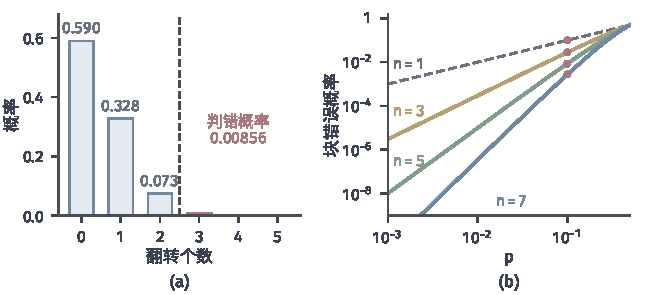
\includegraphics[width=110mm]{figures/07-probability/06-channel-coding/matplotlib/ccode-repetition-flips/figure.pdf}
 \caption{重复码与多数判决。(a) 块长$5$、$p=0.1$时翻转个数的分布$\operatorname{Bin}(5,0.1)$；虚线左侧（蓝）至多两个翻转，一定纠正，右侧（红）一定判错，总概率$0.00856$。(b) 块长$n=1,3,5,7$的块错误概率随翻转概率$p$的变化，双对数坐标；$n=1$（灰色虚线）即不编码，红点标出$p=0.1$处的值。}
 \label{fig:ccode-repetition-flips}
\end{BookInlineFigure}

图~\ref{fig:ccode-repetition-flips}(b)显示了另一面：块长为$2t+1$时，$p$很小的一端曲线的斜率约为$t+1$。原因是式~\eqref{eq:ccode-rep-error}的第一项$\binom{n}{t+1}p^{t+1}(1-p)^{t}$在$p\to0$时起主导作用，错误概率与$p^{t+1}$同阶。能纠正的翻转数$t$决定了噪声变小时错误下降得多快。$p$接近$\tfrac12$时，所有曲线汇合到$\tfrac12$，此时信道输出与输入独立，重复多少遍也没有用。

\paragraph{偶数块长}
块长为偶数时会出现平局。以$n=4$为例，收到两个$0$、两个$1$时，两条消息同样可能，接收端只能任选一个，或者宣布“出错了但不知道是哪条”。所以四次重复码能保证纠正的仍然只有一个翻转，与三次重复码相同，多出来的一次使用只换来了发现两个翻转的能力。区分“发现有错”与“改正错误”，是下一节的主题。

\paragraph{冗余的代价}
重复码的每一份冗余只保护一个消息比特。用三次重复码发送$4$个比特要$12$次信道使用，每个比特独立地以$0.028$的概率出错，$4$位全对的概率是
\[
 (1-0.028)^4\approx0.8926 ,
\]
块错误概率约为$0.107$。不编码时只用$4$次，块错误概率是$1-0.9^4\approx0.344$。三倍的信道使用换来了错误概率的下降，但第~\ref{chap:discrete-channel-capacity}章说明，码率可以接近$0.531$而错误仍趋于零，重复码的$\tfrac13$离此很远。

浪费在哪里？三次重复码把$2^{12}=4096$个可能的接收块分给$16$条消息，平均每条消息占$256$个接收块。但真正需要的只是：每条消息的码字周围，那些“翻转少数几位就能到达”的接收块不要与别的消息混淆。若一个校验位同时参与保护几个消息比特，冗余可以被共享。例如在两个消息比特后面附上它们的模$2$和，任何单个翻转都会让三位之和变成奇数，从而被发现，而码率是$\tfrac23$。只是这一个校验位还不能指出是哪一位出了错。

于是本章面对两个构造问题。一是怎样安排有限的冗余，使不同消息的码字彼此分得足够开，少数翻转之后仍能区分；二是消息很多时，例如$2^{100}$条，怎样不必存储完整的码本，就能完成编码和解码。第~\ref{sec:ccode-min-distance}节用距离回答第一个问题，第~\ref{sec:ccode-linear}节用线性结构回答第二个问题。


\section{最小距离}
\label{sec:ccode-min-distance}

重复码能纠正$t$个翻转，是因为两个码字相差$2t+1$位：从一个码字出发翻转$t$位，离它仍比离另一个码字近。这个观察不依赖于“重复”本身。对任意一个二元码本，两条码字相差几位，决定了翻转之后它们还能不能被区分。

\paragraph{Hamming距离与最小距离}
长度为$n$的二元串记作行向量$\bm{x}$，它的分量是$x_1,\dots,x_n$，全体这样的串记作$\{0,1\}^{n}$。两个串取值不同的位置个数记作$\operatorname{dist}(\bm{x},\bm{y})$，称为\term{Hamming距离}（Hamming distance）。它满足非负、对称、只在$\bm{x}=\bm{y}$时为零，以及三角不等式：$\bm{x},\bm{z}$不同的每个位置上，$\bm{y}$必与其中之一不同，所以这个位置至少计入$\operatorname{dist}(\bm{x},\bm{y})$与$\operatorname{dist}(\bm{y},\bm{z})$之一。这些性质的一般讨论可参考\BookChapterRef{chap:metric-spaces}{卷四第2章“度量空间”}。串中$1$的个数记作$\operatorname{wt}(\bm{x})$，称为\term{Hamming重量}（Hamming weight），它就是$\bm{x}$到全零串的距离。

信道翻转了哪些位置，接收块与码字就在这些位置上不同，所以翻转个数正是接收块到所发码字的Hamming距离。把码本中最近的两条码字之间的距离作为码的指标。

\begin{definition}[最小距离]
\label{def:ccode-min-distance}
设二元码本$\mathcal{C}\subseteq\{0,1\}^{n}$至少含两条码字。它的\term{最小距离}（minimum distance）是
\begin{equation}
 d_{\min}=\min\bigl\{\operatorname{dist}(\bm{c},\bm{c}'):\ \bm{c},\bm{c}'\in\mathcal{C},\ \bm{c}\neq\bm{c}'\bigr\} .
 \label{eq:ccode-dmin}
\end{equation}
\end{definition}

长度为$n$的重复码$d_{\min}=n$。再看一个本章反复使用的码本，它有$4$条长度为$5$的码字：
\[
 \mathcal{C}_5=\{00000,\ 10110,\ 01011,\ 11101\} .
\]
六对码字的距离依次计算：
\[
 \begin{gathered}
 \operatorname{dist}(00000,10110)=3,\quad \operatorname{dist}(00000,01011)=3,\\
 \operatorname{dist}(00000,11101)=4,\quad \operatorname{dist}(10110,01011)=4,\\
 \operatorname{dist}(10110,11101)=3,\quad \operatorname{dist}(01011,11101)=3 .
 \end{gathered}
\]
所以$d_{\min}=3$。它与三次重复码有相同的最小距离，码率却是$\log_24/5=0.4$，高于$\tfrac13$。

\paragraph{检测与纠正}
接收端可以做两件程度不同的事。\term{检错}（error detection）只判断接收块是不是码字：若不是，就知道出了错，可以要求重发或丢弃。\term{纠错}（error correction）还要给出发送的是哪条码字。纠错用的规则是\term{最小距离译码}（minimum-distance decoding）：把接收块判为离它最近的码字，并列时按事先约定的规则任取其一。第~\ref{chap:discrete-channel-capacity}章已经说明，在$p<\tfrac12$的二元对称信道上，码字的似然$p^{k}(1-p)^{n-k}$随距离$k$增大而减小，所以最小距离译码就是最大似然解码。

\begin{theorem}[最小距离的保证]
\label{thm:ccode-detect-correct}
设码本$\mathcal{C}$的最小距离为$d_{\min}$，发送码字$\bm{c}\in\mathcal{C}$，接收块$\bm{y}$与$\bm{c}$相差$j$位。
\begin{enumerate}
 \item 若$1\leq j\leq d_{\min}-1$，则$\bm{y}\notin\mathcal{C}$，错误一定被检测到。
 \item 若
 \begin{equation}
  j\leq t,\qquad t=\Bigl\lfloor\frac{d_{\min}-1}{2}\Bigr\rfloor ,
  \label{eq:ccode-correct-radius}
 \end{equation}
 则$\bm{c}$是离$\bm{y}$最近的唯一码字，最小距离译码一定判对。
\end{enumerate}
\end{theorem}

\begin{proof}
(1) $\bm{y}$与$\bm{c}$不同，且距离$j$小于$d_{\min}$。若$\bm{y}$是码字，它就是与$\bm{c}$不同、距离小于$d_{\min}$的码字，与最小距离的定义矛盾。

(2) 由$t$的定义，$2t\leq d_{\min}-1$，即$2t<d_{\min}$。对任一码字$\bm{c}'\neq\bm{c}$，三角不等式给出
\[
 d_{\min}\leq\operatorname{dist}(\bm{c},\bm{c}')\leq\operatorname{dist}(\bm{c},\bm{y})+\operatorname{dist}(\bm{y},\bm{c}') .
\]
移项并代入$\operatorname{dist}(\bm{c},\bm{y})=j\leq t$，得到
\[
 \operatorname{dist}(\bm{y},\bm{c}')\geq d_{\min}-j\geq d_{\min}-t>t\geq j .
\]
所以每个其他码字都比$\bm{c}$离$\bm{y}$更远，最近的码字唯一，就是$\bm{c}$。
\end{proof}

对$\mathcal{C}_5$，$d_{\min}=3$，保证检测至多$2$个翻转、纠正$1$个翻转。图~\ref{fig:ccode-distance-chain}用重复码说明两个半径怎样产生。(a)中$d_{\min}=5$，两条码字之间相隔五步，各自往中间走两步的范围不相交，所以两个翻转可以纠正；任何不超过四步的走法都到不了另一端，所以四个翻转可以检测。(b)中$d_{\min}=4$，正中间的$1100$离两端都是两步，两个翻转只能被发现，不能被纠正。

\begin{BookInlineFigure}
 \centering
 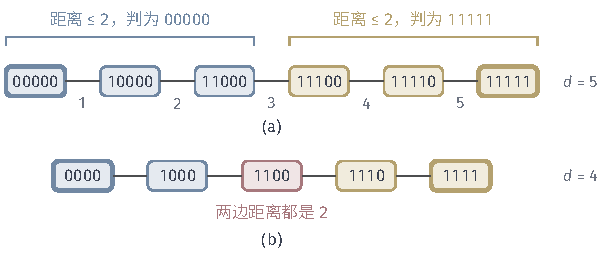
\includegraphics[width=103.2mm]{figures/07-probability/06-channel-coding/tikz/ccode-distance-chain/figure.pdf}
 \caption{沿一条每步翻转一位的路径，从一个码字走到另一个码字（粗框）。(a) 长度$5$的重复码，$d_{\min}=5$：距$00000$不超过$2$的串（蓝）判为$00000$，距$11111$不超过$2$的串（黄）判为$11111$，两部分不相交。(b) 长度$4$的重复码，$d_{\min}=4$：中间的$1100$（红）到两个码字的距离都是$2$。}
 \label{fig:ccode-distance-chain}
\end{BookInlineFigure}

\paragraph{判决球}
定理~\ref{thm:ccode-detect-correct}的第二条有一个几何读法。以码字$\bm{c}$为中心、半径为$t$的Hamming球
\[
 B(\bm{c},t)=\bigl\{\bm{y}\in\{0,1\}^{n}:\ \operatorname{dist}(\bm{y},\bm{c})\leq t\bigr\}
\]
是“翻转不超过$t$个”所能到达的全部接收块。证明中的不等式说明，当$2t<d_{\min}$时，不同码字的球互不相交：若$\bm{y}$同时在两个球内，它到两个中心的距离之和不超过$2t$，与两中心距离至少$d_{\min}$矛盾。互不相交的球给每条码字划出了一块专属的领地，落在领地里的接收块只有一种合理的解释。

图~\ref{fig:ccode-decoding-balls}是这一图景的示意。落在某个球里的接收块$y_1$被纠正到球心；落在所有球之外的$y_2$离每个码字都超过$t$，接收端知道出了错，但定理不保证它会被判对。检测的半径更大：从一个码字出发翻转不到$d_{\min}$位，到不了别的码字，所以只要接收块不是码字，就能发现错误。

\begin{BookInlineFigure}
 \centering
 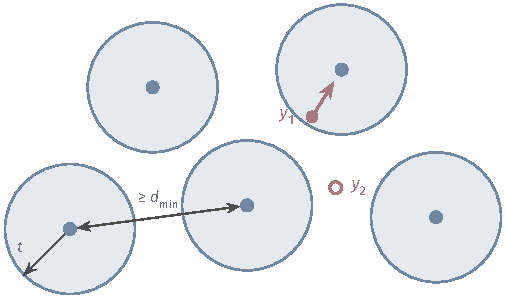
\includegraphics[width=85.7mm]{figures/07-probability/06-channel-coding/tikz/ccode-decoding-balls/figure.pdf}
 \caption{Hamming空间中判决球的示意（平面上的圆只表示“距离不超过$t$”的集合，不按真实形状绘制）。蓝点为码字，两两距离至少$d_{\min}$；浅蓝圆为半径$t=\lfloor(d_{\min}-1)/2\rfloor$的球，互不相交。红点$y_1$在球内，被纠正到球心；空心红点$y_2$不在任何球内，只能确定出了错。}
 \label{fig:ccode-decoding-balls}
\end{BookInlineFigure}

用$\mathcal{C}_5$数一数这些领地。长度为$5$的串共有$32$个，每个半径为$1$的球含中心本身和$5$个只差一位的串，共$6$个。四个球互不相交，合计$24$个串，剩下$8$个串不在任何球内。这$8$个串每个都与某两条码字相距$2$，例如$00101$到$00000$与$11101$的距离都是$2$，到另外两条码字的距离都是$3$。

\paragraph{超出半径之后}
翻转个数超过$t$时，定理不作任何承诺，但这不等于一定判错。$\mathcal{C}_5$上翻转两位后，接收块可能落进另一条码字的球里，也可能落在那$8$个“无主”的串上；后一种情形下，最小距离译码要在两条并列最近的码字中选一个，选中原码字的机会是存在的。所以超出半径后的错误概率，要按具体的信道、具体的码和具体的判决规则（包括并列时怎样选）来计算。只用保证半径计算，能得到的是错误概率的上界：在$p=0.1$时，
\[
 P_{\mathrm{e}}\leq\mathbb{P}(\text{翻转个数}\geq2)=1-0.9^5-5\times0.1\times0.9^4=0.08146 .
\]
第~\ref{sec:ccode-syndrome}小节给出一个具体的并列规则，精确算出它的错误概率。


\section{二元线性码}
\label{sec:ccode-linear}

传送$100$个比特的消息，码本有$2^{100}$条码字，无法逐条写下来，也无法逐条比较。需要一种结构，让码字可以按规则现场算出，让接收端只做少量运算就能判断接收块是否合法、错在哪里。$\mathcal{C}_5$已经暗示了这种结构：$10110$与$01011$逐位模$2$相加，恰好得到第四条码字$11101$。

\paragraph{模2运算}
在$\{0,1\}$上规定加法为模$2$加法，乘法为普通乘法：
\[
 0+0=0,\quad 0+1=1+0=1,\quad 1+1=0,\qquad 0\cdot x=0,\quad 1\cdot x=x .
\]
加法就是“异或”，$1$加两次回到原处，所以每个元素的负元是它自己，减法与加法相同。这两种运算满足交换律、结合律、分配律，$1$有乘法逆元$1$，所以$\{0,1\}$在这两种运算下构成一个只有两个元素的域，称为\term{二元域}（binary field），记作$\mathbb{F}_2$。

长度为$n$的二元串逐位相加、逐位乘以$0$或$1$，就构成$\mathbb{F}_2$上的$n$维线性空间$\mathbb{F}_2^{n}$。线性无关、基、维数、秩、零空间以及秩与零空间维数之和等于列数的结论，推导中只用到域的四则运算，所以在$\mathbb{F}_2$上照样成立，Gauss消元也照样可用，只是每一步都按模$2$计算。这些结论在实数域上的叙述可参考\BookChapterRef{chap:linear-representation}{卷二第2章“线性空间、映射与坐标”}。$\mathbb{F}_2^{n}$只有有限个向量，一个$k$维子空间恰有$2^{k}$个向量，因为每个向量由它在一组基下的$k$个系数唯一确定，每个系数有两种取法。

与实数空间的一个不同是，$\mathbb{F}_2^{n}$中的非零向量可以与自身“正交”：$(1,1)$与自身逐位相乘再相加得$1+1=0$。所以下面不使用正交投影的直觉，只使用秩与零空间。

\begin{definition}[二元线性码]
\label{def:ccode-linear-code}
$\mathbb{F}_2^{n}$的一个$k$维线性子空间$\mathcal{C}$称为$[n,k]$\term{二元线性码}（binary linear code）。它含$M=2^{k}$条码字，码率为
\begin{equation}
 R=\frac{\log_2M}{n}=\frac{k}{n} .
 \label{eq:ccode-linear-rate}
\end{equation}
若还知道最小距离为$d_{\min}$，就记作$[n,k,d_{\min}]$码。
\end{definition}

式~\eqref{eq:ccode-linear-rate}就是第~\ref{chap:discrete-channel-capacity}章块码码率$\log_2M/n$在$M=2^{k}$时的值：一条码字承载$k$个消息比特，用$n$次信道。检查$\mathcal{C}_5$是子空间，只需验证它含零向量且对加法封闭：
\[
 10110+01011=11101,\quad 10110+11101=01011,\quad 01011+11101=10110 ,
\]
码字与自身相加得$00000$。所以$\mathcal{C}_5$是$[5,2,3]$码。长度为$n$的重复码$\{0\cdots0,\,1\cdots1\}$是$[n,1,n]$码。

\paragraph{距离化为重量}
线性结构立刻简化了最小距离的计算。两条码字不同的位置，正是它们的和为$1$的位置，所以
\[
 \operatorname{dist}(\bm{c},\bm{c}')=\operatorname{wt}(\bm{c}+\bm{c}') .
\]

\begin{lemma}[线性码的最小距离]
\label{lem:ccode-min-weight}
线性码的最小距离等于非零码字的最小重量：
\begin{equation}
 d_{\min}=\min\{\operatorname{wt}(\bm{c}):\ \bm{c}\in\mathcal{C},\ \bm{c}\neq\bm{0}\} .
 \label{eq:ccode-min-weight}
\end{equation}
\end{lemma}

\begin{proof}
对两条不同码字，$\bm{c}+\bm{c}'$是非零码字，由上式它们的距离就是这条码字的重量，所以$d_{\min}$不小于右边。反过来，对任一非零码字$\bm{c}$，$\bm{0}$也是码字，它的重量就是它到$\bm{0}$的距离，不小于$d_{\min}$，且取到最小重量的那条码字给出等号。
\end{proof}

一般码本要比较$M(M-1)/2$对码字，线性码只需检查$M-1$条非零码字的重量。$\mathcal{C}_5$的非零码字重量是$3,3,4$，最小距离为$3$，与上一节逐对计算的结果一致。线性码还有一个性质：从任何一条码字看出去，其他码字的距离分布都一样，因为加上一条固定码字把码本映成它自身，并保持距离不变。所以分析一条码字（通常取全零码字）的错误，就是在分析所有码字。

\subsection{生成矩阵}
\label{sec:ccode-generator}

一个$k$维子空间由它的任意一组基确定。把基向量作为行排成矩阵，就能用矩阵乘法从消息算出码字。

\begin{definition}[生成矩阵]
\label{def:ccode-generator}
设$\bm{G}\in\mathbb{F}_2^{k\times n}$的秩为$k$，它的行张成$[n,k]$码$\mathcal{C}$。称$\bm{G}$为$\mathcal{C}$的\term{生成矩阵}（generator matrix），编码规则为
\begin{equation}
 \bm{u}\mapsto\bm{c}=\bm{u}\bm{G},\qquad \bm{u}\in\mathbb{F}_2^{k},
 \label{eq:ccode-encode}
\end{equation}
运算按模$2$进行，消息$\bm{u}$与码字$\bm{c}$都是行向量。
\end{definition}

秩为$k$保证消息可以唯一恢复。若$\bm{u}\bm{G}=\bm{u}'\bm{G}$，则$(\bm{u}+\bm{u}')\bm{G}=\bm{0}$，这是$\bm{G}$的各行以$\bm{u}+\bm{u}'$的分量为系数的组合；行线性无关，只能有$\bm{u}+\bm{u}'=\bm{0}$，即$\bm{u}=\bm{u}'$。所以式~\eqref{eq:ccode-encode}是从$2^{k}$条消息到$2^{k}$条码字的一一对应。若$\bm{G}$的秩小于$k$，就有两条不同的消息被编成同一条码字，接收端无论如何也无法区分它们。

\paragraph{系统形式}
若生成矩阵的前$k$列是单位矩阵，
\begin{equation}
 \bm{G}=\bigl[\,\bm{I}_k\ \ \bm{A}\,\bigr],\qquad \bm{A}\in\mathbb{F}_2^{k\times(n-k)},
 \label{eq:ccode-systematic}
\end{equation}
称它为\term{系统形式}（systematic form）。这时码字是$\bm{c}=(\bm{u},\ \bm{u}\bm{A})$：前$k$位照抄消息，称为消息位；后$n-k$位是消息比特的若干模$2$和，称为校验位。接收端纠正错误以后，直接读出前$k$位就得到消息。

任何线性码都可以化成这种形式，至多需要重排列的顺序。对$\bm{G}$作行的初等变换（交换两行、把一行加到另一行），行空间不变，码本也不变；化成约化行阶梯形后，主元所在的$k$列构成单位矩阵。把这些列移到最前面，等于对所有码字同时重排坐标，各码字之间的距离不变。

\paragraph{$[5,2,3]$码的编码}
$\mathcal{C}_5$的生成矩阵可以取系统形式
\[
 \bm{G}_5=\begin{pmatrix}1&0&1&1&0\\ 0&1&0&1&1\end{pmatrix},
 \qquad
 \bm{A}=\begin{pmatrix}1&1&0\\ 0&1&1\end{pmatrix} .
\]
消息$\bm{u}=(u_1,u_2)$编成
\[
 \bm{c}=(u_1,\ u_2,\ u_1,\ u_1+u_2,\ u_2) .
\]
例如$\bm{u}=(1,1)$时，$\bm{c}=\bm{u}\bm{G}_5$是两行之和，即$10110+01011=11101$。图~\ref{fig:ccode-generator-map}画出每个码字位由哪些消息比特决定，以及全部四条码字。

\begin{BookInlineFigure}
 \centering
 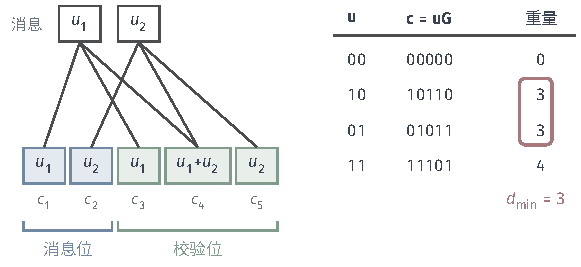
\includegraphics[width=98.3mm]{figures/07-probability/06-channel-coding/tikz/ccode-generator-map/figure.pdf}
 \caption{$[5,2,3]$码的系统编码$\bm{c}=\bm{u}\bm{G}_5$。左：$c_1,c_2$（蓝）照抄消息，$c_3,c_4,c_5$（绿）是消息比特的模$2$和，连线表示参与求和的比特。右：四条消息及其码字和重量，红框标出最小非零重量$3$，即最小距离。}
 \label{fig:ccode-generator-map}
\end{BookInlineFigure}

\paragraph{结构节省了什么}
存储整个码本需要$2^{k}\times n$个比特，存储生成矩阵只要$k\times n$个比特。编码一条消息是把$\bm{G}$中对应$u_i=1$的行相加，至多$k(n-k)$次比特加法（系统形式下消息位不用算）。$k=100$、$n=200$时，码本有$2^{100}$行，生成矩阵只有$100$行。线性结构解决了存储与编码的问题，解码则需要下面的校验矩阵。

\subsection{校验矩阵}
\label{sec:ccode-parity-check}

生成矩阵描述码字“怎样产生”。接收端需要的是另一种描述：给一个接收块，怎样快速判断它是不是码字。$\mathcal{C}_5$的码字满足三条关系$c_3=c_1$，$c_4=c_1+c_2$，$c_5=c_2$，在模$2$下移项，就是三个和为零的方程：
\[
 c_1+c_3=0,\qquad c_1+c_2+c_4=0,\qquad c_2+c_5=0 .
\]
把这些方程的系数排成矩阵，码本就成为它的零空间。

\begin{definition}[校验矩阵]
\label{def:ccode-parity-check}
设$\bm{H}\in\mathbb{F}_2^{(n-k)\times n}$的秩为$n-k$。若
\begin{equation}
 \mathcal{C}=\bigl\{\bm{c}\in\mathbb{F}_2^{n}:\ \bm{H}\bm{c}^{\top}=\bm{0}\bigr\},
 \label{eq:ccode-null-space}
\end{equation}
称$\bm{H}$为$[n,k]$码$\mathcal{C}$的\term{校验矩阵}（parity-check matrix）。$\bm{H}$的每一行给出一条校验方程。
\end{definition}

\begin{lemma}[由系统形式构造校验矩阵]
\label{lem:ccode-h-from-g}
若$\bm{G}=[\,\bm{I}_k\ \ \bm{A}\,]$，则
\begin{equation}
 \bm{H}=\bigl[\,\bm{A}^{\top}\ \ \bm{I}_{n-k}\,\bigr]
 \label{eq:ccode-h-systematic}
\end{equation}
是同一个码的校验矩阵，并且
\begin{equation}
 \bm{G}\bm{H}^{\top}=\bm{0} .
 \label{eq:ccode-gh}
\end{equation}
\end{lemma}

\begin{proof}
分块相乘，
\[
 \bm{G}\bm{H}^{\top}=\bm{I}_k\bm{A}+\bm{A}\bm{I}_{n-k}=\bm{A}+\bm{A}=\bm{0},
\]
最后一步用到模$2$下$x+x=0$。于是$\bm{G}$的每一行都满足$\bm{H}\bm{g}^{\top}=\bm{0}$；零空间是子空间，行的任意组合也满足，所以$\mathcal{C}$包含在$\bm{H}$的零空间中。

$\bm{H}$含单位矩阵$\bm{I}_{n-k}$作为子块，所以秩为$n-k$，由秩与零空间维数之和等于列数$n$，零空间的维数是$k$。$\mathcal{C}$是这个$k$维空间的$k$维子空间，两者相等。
\end{proof}

相容条件~\eqref{eq:ccode-gh}的含义是：生成矩阵的每一行都通过全部校验。它与秩的条件一起，就足以说明两个矩阵描述同一个码；验证一个给定的$\bm{H}$时不必列出全部码字。对$\mathcal{C}_5$，$\bm{A}^{\top}$是$3\times2$矩阵，
\[
 \bm{H}_5=\begin{pmatrix}1&0&1&0&0\\ 1&1&0&1&0\\ 0&1&0&0&1\end{pmatrix} .
\]
它的三行正是上面的三条校验方程。检查第一行生成向量$10110$：三条方程依次给出$1+1=0$，$1+0+1=0$，$0+0=0$，全部通过。

\paragraph{错误向量}
二元对称信道翻转哪些位置，可以用一个错误向量$\bm{e}\in\mathbb{F}_2^{n}$记录：$e_i=1$表示第$i$位被翻转。翻转就是加$1$，所以接收块是
\begin{equation}
 \bm{y}=\bm{c}+\bm{e} .
 \label{eq:ccode-error-model}
\end{equation}
在二元对称信道上，$e_1,\dots,e_n$相互独立，都服从$\operatorname{Bern}(p)$，并且与发送的码字独立。一个具体错误向量的概率只依赖它的重量：
\[
 \mathbb{P}(\bm{e})=p^{\operatorname{wt}(\bm{e})}(1-p)^{n-\operatorname{wt}(\bm{e})} .
\]

用校验矩阵作用于接收块，码字的部分消失了：
\begin{equation}
 \bm{H}\bm{y}^{\top}=\bm{H}\bm{c}^{\top}+\bm{H}\bm{e}^{\top}=\bm{H}\bm{e}^{\top} .
 \label{eq:ccode-syndrome-error}
\end{equation}
接收端不知道$\bm{c}$也不知道$\bm{e}$，但能算出左边；右边说明这个量只取决于信道造成的错误，与发送哪条消息无关。它是接收端能够直接计算、又只携带错误信息的量，下一小节用它定位错误。

\paragraph{一次校验}
发送$\bm{c}=10110$，信道翻转第$3$位，收到$\bm{y}=10010$。三条校验依次为
\[
 y_1+y_3=1+0=1,\qquad y_1+y_2+y_4=1+0+1=0,\qquad y_2+y_5=0+0=0 .
\]
只有第一条不通过。图~\ref{fig:ccode-check-graph}把每条校验画成连接若干位置的方框：第一条校验连接位置$1$和$3$，但位置$1$还参与第二条校验，而第二条校验通过了，所以单个翻转只能在位置$3$。这就是用校验结果定位错误的思路。

\begin{BookInlineFigure}
 \centering
 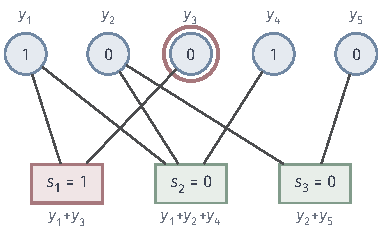
\includegraphics[width=64.7mm]{figures/07-probability/06-channel-coding/tikz/ccode-check-graph/figure.pdf}
 \caption{$[5,2,3]$码的校验关系，上方圆圈为接收块$\bm{y}=10010$的各位，下方方框为$\bm{H}_5$的三条校验，连线表示参与该校验的位置。红色方框是不通过的校验，红圈标出被翻转的第$3$位。}
 \label{fig:ccode-check-graph}
\end{BookInlineFigure}

\paragraph{从校验矩阵读出最小距离}
校验矩阵还能直接判断码能纠正几个错误。记$\bm{H}$的第$j$列为$\bm{h}_j$。若$\bm{c}$在位置集合$S$上为$1$、其余为$0$，则$\bm{H}\bm{c}^{\top}=\sum_{j\in S}\bm{h}_j$。所以$\bm{c}$是码字，当且仅当它为$1$的那些列相加为零。

\begin{lemma}[由校验列判断最小距离]
\label{lem:ccode-columns}
$[n,k]$码的最小距离至少为$3$，当且仅当其校验矩阵的各列都非零且两两不同。
\end{lemma}

\begin{proof}
由引理~\ref{lem:ccode-min-weight}，最小距离至少为$3$等价于没有重量为$1$或$2$的非零码字。重量为$1$、在位置$j$上为$1$的码字存在，当且仅当$\bm{h}_j=\bm{0}$。重量为$2$、在位置$i\neq j$上为$1$的码字存在，当且仅当$\bm{h}_i+\bm{h}_j=\bm{0}$，即$\bm{h}_i=\bm{h}_j$。两种情形都排除，就是各列非零且互不相同。
\end{proof}

$\bm{H}_5$的五列是$110,011,100,010,001$（按列从上到下读），互不相同且非零，所以$d_{\min}\geq3$；第$1$、$3$、$4$列之和为$110+100+010=000$，对应重量为$3$的码字$10110$，所以$d_{\min}=3$。这条引理把“设计纠单错的码”变成了“选一些互不相同的非零列”，第~\ref{sec:ccode-hamming}节正是这样构造Hamming码的。

\subsection{综合征译码}
\label{sec:ccode-syndrome}

式~\eqref{eq:ccode-syndrome-error}给出了只依赖错误的量。它能确定错误吗？在$\mathcal{C}_5$上，校验结果只有$2^{3}=8$种，而可能的错误向量有$32$个，平均每种校验结果对应$4$个错误。接收端要在这$4$个候选中选出最可能的一个。

\begin{definition}[综合征]
\label{def:ccode-syndrome}
设$\bm{H}$是$[n,k]$码的校验矩阵。接收块$\bm{y}$的\term{综合征}（syndrome）是
\begin{equation}
 \bm{s}=\bm{H}\bm{y}^{\top}\in\mathbb{F}_2^{\,n-k} .
 \label{eq:ccode-syndrome}
\end{equation}
\end{definition}

综合征为零，当且仅当$\bm{y}$是码字。所以检错只需计算一次综合征，不为零就报告出错，代价是$(n-k)\times n$次比特运算。

\paragraph{主要思想}
综合征为$\bm{s}$时，哪些错误向量与它相容？若$\bm{e}_0$是其中一个，即$\bm{H}\bm{e}_0^{\top}=\bm{s}$，则$\bm{H}\bm{e}^{\top}=\bm{s}$当且仅当$\bm{H}(\bm{e}+\bm{e}_0)^{\top}=\bm{0}$，即$\bm{e}+\bm{e}_0\in\mathcal{C}$。所以相容的错误向量恰好组成集合
\begin{equation}
 \bm{e}_0+\mathcal{C}=\{\bm{e}_0+\bm{c}:\ \bm{c}\in\mathcal{C}\},
 \label{eq:ccode-coset}
\end{equation}
它是码空间平移后得到的\term{陪集}（coset），含$2^{k}$个向量。不同的综合征对应不相交的陪集，$2^{n-k}$个陪集恰好把$\mathbb{F}_2^{n}$分成大小相同的$2^{n-k}$块。

接收端观察到$\bm{y}$后，真实的错误一定在$\bm{y}$所在的陪集$\bm{y}+\mathcal{C}$里（因为$\bm{e}=\bm{y}+\bm{c}$），这正是综合征为$\bm{H}\bm{y}^{\top}$的陪集。陪集中每个候选$\bm{e}$对应一个候选码字$\bm{y}+\bm{e}$。由错误向量的概率只依赖重量，当$p<\tfrac12$时，$p^{w}(1-p)^{n-w}$随$w$增大而减小，最可能的错误就是陪集中重量最小的向量。

\begin{definition}[陪集首与综合征译码]
\label{def:ccode-syndrome-decoding}
在每个陪集中选定一个重量最小的向量$\hat{\bm{e}}(\bm{s})$，称为该陪集的\term{陪集首}（coset leader）。\term{综合征译码}（syndrome decoding）把接收块$\bm{y}$译为
\begin{equation}
 \hat{\bm{c}}=\bm{y}+\hat{\bm{e}}\bigl(\bm{H}\bm{y}^{\top}\bigr) .
 \label{eq:ccode-syndrome-decode}
\end{equation}
\end{definition}

$\hat{\bm{c}}$一定是码字：$\bm{y}$与$\hat{\bm{e}}$在同一陪集中，它们的和属于$\mathcal{C}$。它也是离$\bm{y}$最近的码字，因为$\bm{y}$到码字$\bm{c}$的距离是$\bm{y}+\bm{c}$的重量，而$\bm{y}+\bm{c}$在$\bm{c}$取遍$\mathcal{C}$时恰好取遍这个陪集。所以综合征译码就是最小距离译码，陪集首的选择就是并列时的选择规则；在$p<\tfrac12$的二元对称信道上，它是最大似然解码。

把$\mathbb{F}_2^{n}$按陪集逐行排开，每行以陪集首开头，按列对齐码字，得到的表称为\term{标准阵}（standard array）。接收块所在的列顶端就是译码结果。实际译码只需存储综合征到陪集首的对照表，共$2^{n-k}$项，不需要标准阵本身。

\paragraph{计算过程}
用$\mathcal{C}_5$走一遍。

\needspace{6\baselineskip}
\paragraph{变量}
\begin{itemize}
 \item 校验矩阵$\bm{H}_5$，$3\times5$；
 \item 对照表：$8$个综合征$\bm{s}\in\mathbb{F}_2^{3}$各对应一个陪集首$\hat{\bm{e}}(\bm{s})\in\mathbb{F}_2^{5}$；
 \item 每个接收块$\bm{y}$（$1\times5$）、它的综合征$\bm{s}$（$3\times1$）、纠正后的码字$\hat{\bm{c}}$与消息$\hat{\bm{u}}$（$1\times2$）。
\end{itemize}

\paragraph{初始化}
对照表在收到任何数据之前一次建好。按重量从小到大枚举错误向量，同重量的按位置组合的字典序，算出综合征；某个综合征第一次出现时，记下这个向量作为它的陪集首，$8$个综合征都出现后停止。

例中重量$0$的$00000$给出$\bm{s}=000$。重量$1$的向量在位置$j$为$1$，综合征是第$j$列，依次得到
\[
 \begin{gathered}
 10000\mapsto110,\quad 01000\mapsto011,\quad 00100\mapsto100,\\
 00010\mapsto010,\quad 00001\mapsto001 .
 \end{gathered}
\]
还剩$101$与$111$。重量$2$的向量按位置对$(1,2),(1,3),\dots$枚举：$11000$的综合征是第$1$、$2$列之和
\[
 110+011=101 ,
\]
记下$\hat{\bm{e}}(101)=11000$；接着$10100\mapsto010$、$10010\mapsto100$都已出现；$10001\mapsto110+001=111$，记下$\hat{\bm{e}}(111)=10001$。对照表完成。

\needspace{6\baselineskip}
\paragraph{每轮更新}
每收到一个接收块执行一轮：
\begin{enumerate}
 \item 由式~\eqref{eq:ccode-syndrome}算综合征$\bm{s}=\bm{H}_5\bm{y}^{\top}$。例中第一轮收到$\bm{y}=10010$（发送$10110$，第$3$位翻转），上一小节已算出
 \[
  \bm{s}=100 .
 \]
 \item 查表得$\hat{\bm{e}}(\bm{s})$。例中第一轮$\hat{\bm{e}}(100)=00100$。
 \item 由式~\eqref{eq:ccode-syndrome-decode}纠正，再读出前两位作为消息。例中第一轮
 \[
  \hat{\bm{c}}=10010+00100=10110,\qquad \hat{\bm{u}}=10 ,
 \]
 与发送的消息一致。
\end{enumerate}
第二轮发送同一条码字$10110$，信道翻转第$3$、$5$两位，$\bm{e}=00101$，收到$\bm{y}=10011$。三条校验给出
\[
 s_1=1+0=1,\qquad s_2=1+0+1=0,\qquad s_3=0+1=1 ,
\]
即$\bm{s}=101$。查表得$\hat{\bm{e}}=11000$，于是
\[
 \hat{\bm{c}}=10011+11000=01011,\qquad \hat{\bm{u}}=01 ,
\]
译错了。真实错误$00101$与陪集首$11000$在同一陪集中，重量都是$2$，在二元对称信道上出现的概率相同，接收端没有任何依据区分它们。每个接收块只需一次综合征计算和一次查表，处理完全部接收块即结束。最终得到：单个翻转都被纠正，两个翻转是否被纠正取决于它是否恰好是陪集首。

图~\ref{fig:ccode-standard-array}是$\mathcal{C}_5$的标准阵。第一行是码本，每一行是一个陪集，左边是它的综合征。最后两行的陪集中有两个重量为$2$的向量，陪集首只能选其中一个；另一个错误模式（红框）出现时，接收块所在列顶端的码字就不是原码字。第二轮的接收块$10011$位于综合征$101$那一行、码字$01011$那一列。

\begin{BookInlineFigure}
 \centering
 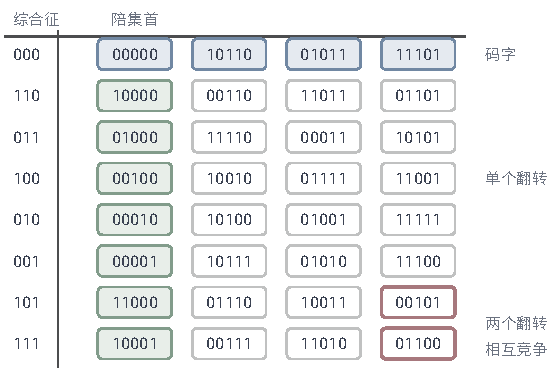
\includegraphics[width=94.6mm]{figures/07-probability/06-channel-coding/tikz/ccode-standard-array/figure.pdf}
 \caption{$[5,2,3]$码的标准阵：$32$个长度为$5$的串分成$8$个陪集，每行一个，左列为综合征。第一行（蓝）是码本，第一列（绿）是按正文枚举顺序选出的陪集首，每个串都等于所在行的陪集首加上所在列顶端的码字。最后两行各有两个重量为$2$的串，未被选为陪集首的那个用红框标出。}
 \label{fig:ccode-standard-array}
\end{BookInlineFigure}

\paragraph{错误概率}
综合征译码何时判对？由式~\eqref{eq:ccode-error-model}与式~\eqref{eq:ccode-syndrome-decode}，
\[
 \hat{\bm{c}}=\bm{c}+\bm{e}+\hat{\bm{e}}(\bm{H}\bm{e}^{\top}) .
\]
$\bm{e}$与$\hat{\bm{e}}$在同一陪集，它们的和是码字；$\hat{\bm{c}}=\bm{c}$当且仅当这个和为零，即真实错误恰好是陪集首。这一条件与发送哪条码字无关，所以每条消息的条件错误概率相同，平均错误与最大错误相等：
\begin{equation}
 1-P_{\mathrm{e}}=\sum_{\bm{s}\in\mathbb{F}_2^{n-k}}p^{\operatorname{wt}(\hat{\bm{e}}(\bm{s}))}(1-p)^{n-\operatorname{wt}(\hat{\bm{e}}(\bm{s}))} .
 \label{eq:ccode-syndrome-success}
\end{equation}

$\mathcal{C}_5$的陪集首有$1$个重量$0$、$5$个重量$1$、$2$个重量$2$。在$p=0.1$时，三类的贡献分别是
\[
 0.9^5=0.59049,\qquad 5\times0.1\times0.9^4=0.32805,\qquad 2\times0.1^2\times0.9^3=0.01458 .
\]
相加得到
\[
 1-P_{\mathrm{e}}=0.93312,\qquad P_{\mathrm{e}}=0.06688 .
\]
这比上一节只用保证半径得到的上界$0.08146$小，差额$0.01458$正是被“碰巧纠对”的两个翻转。图~\ref{fig:ccode-beyond-radius}按错误重量分组显示这一点：重量不超过$1$的错误全部纠正；$10$个重量为$2$的错误中只有$2$个是陪集首；重量$3$及以上的错误一个也纠不了。作为对照，用三次重复码发送两个比特要$6$次信道，块错误概率为$1-0.972^2\approx0.0552$；$\mathcal{C}_5$少用一次信道，错误概率略高。

\begin{BookInlineFigure}
 \centering
 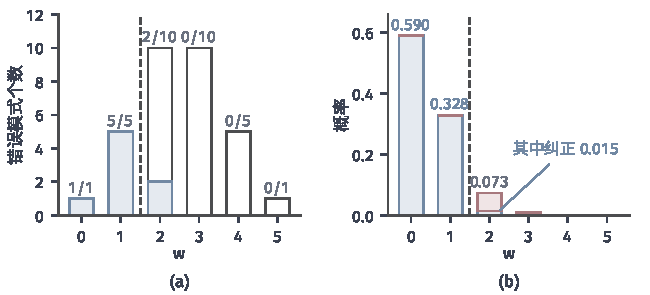
\includegraphics[width=110mm]{figures/07-probability/06-channel-coding/matplotlib/ccode-beyond-radius/figure.pdf}
 \caption{$[5,2,3]$码在$p=0.1$的二元对称信道上用综合征译码，按错误向量的重量$w$分组。(a) 每组错误模式的个数（白柱）与其中被选为陪集首、因而被纠正的个数（蓝），柱顶为二者之比；虚线左侧在保证半径$t=1$之内。(b) 每组的概率，蓝色为被纠正的部分，红色为未被纠正的部分；$w=2$的一组概率$0.073$中只有$0.015$被纠正。}
 \label{fig:ccode-beyond-radius}
\end{BookInlineFigure}

\paragraph{三件不同的事}
综合征译码把接收端可以做的事分成三个层次。检测非法码字只看综合征是否为零，对任何线性码都便宜。选出最可能的错误要在陪集中找最小重量的向量，这是一个依赖信道的判断：在二元对称信道上是最小重量，在别的信道上要改用相应的似然。保证唯一纠错则是关于码本身的结论：重量不超过$t$的错误在各自的陪集中是唯一的最小重量向量，由定理~\ref{thm:ccode-detect-correct}，它们一定被纠正，而超过$t$的错误可能与别的向量并列，甚至不是陪集中重量最小的。

\paragraph{译码的代价}
线性结构把编码变成了矩阵乘法，但没有自动让译码变得容易。对照表有$2^{n-k}$项，冗余位数$n-k$稍大，表就无法存储：$n=1000$、$k=500$时有$2^{500}$项。不建表而在陪集中现场寻找最小重量向量，需要搜索的向量同样多。对于一般的线性码，目前没有已知的方法能在块长的多项式时间内完成最大似然译码。所以“线性”只是可计算的起点；要得到可以实际使用的长码，还需要更多的代数结构或专门设计的迭代译码方法，这超出了本章的范围。下一节的Hamming码是一个结构使译码变得非常简单的例子。


\section{Hamming码}
\label{sec:ccode-hamming}

引理~\ref{lem:ccode-columns}说，只要校验矩阵的各列非零且互不相同，码就能纠正任意一个翻转。校验矩阵有$r=n-k$行时，非零的列向量一共只有$2^{r}-1$个，所以块长至多为$2^{r}-1$。把它们全部用上，就在给定的冗余位数下得到最长、码率最高的纠单错码，这就是\term{Hamming码}（Hamming code）。$r=3$时，$n=7$，$k=4$，这正是本章开头要找的码：用$7$次信道发送$4$个比特，任何一位翻转都能改回来。

\paragraph{校验矩阵与校验位置}
把$7$个非零的三维列向量按“第$j$列是$j$的二进制表示”排列，最上面一行是最低位：
\begin{equation}
 \bm{H}_7=\begin{pmatrix}
 1&0&1&0&1&0&1\\
 0&1&1&0&0&1&1\\
 0&0&0&1&1&1&1
 \end{pmatrix} .
 \label{eq:ccode-hamming-h}
\end{equation}
例如第$5$列是$(1,0,1)^{\top}$，自下而上读作$101$，正是二进制的$5$。三行分别要求位置$\{1,3,5,7\}$、$\{2,3,6,7\}$、$\{4,5,6,7\}$上的比特之和为偶数。

第$1$、$2$、$4$列是单位向量，各自只出现在一条校验中。可以让这三个位置专门承担校验，其余位置$3,5,6,7$放消息比特$u_1,u_2,u_3,u_4$。每条校验恰好含一个校验位置，于是校验位由消息位直接算出：
\begin{equation}
 c_1=c_3+c_5+c_7,\qquad c_2=c_3+c_6+c_7,\qquad c_4=c_5+c_6+c_7 .
 \label{eq:ccode-hamming-parity}
\end{equation}
这与系统形式只差一个坐标排列：消息仍然原样出现在码字中，只是不在最前面。$\bm{H}_7$的秩为$3$（它含三个单位列），所以码空间的维数是$7-3=4$，码率为$\tfrac47$。

\paragraph{编码一条消息}
取消息$\bm{u}=1011$，放入位置$3,5,6,7$：
\[
 c_3=1,\qquad c_5=0,\qquad c_6=1,\qquad c_7=1 .
\]
由式~\eqref{eq:ccode-hamming-parity}算三个校验位：
\[
 c_1=1+0+1=0,\qquad c_2=1+1+1=1,\qquad c_4=0+1+1=0 .
\]
按位置顺序排好，码字是
\[
 \bm{c}=0110011 .
\]
对四个单位消息分别编码，得到生成矩阵的四行，它们满足$\bm{G}_7\bm{H}_7^{\top}=\bm{0}$：
\[
 \bm{G}_7=\begin{pmatrix}
 1&1&1&0&0&0&0\\
 1&0&0&1&1&0&0\\
 0&1&0&1&0&1&0\\
 1&1&0&1&0&0&1
 \end{pmatrix} .
\]
上面的码字也等于第$1$、$3$、$4$行之和，与式~\eqref{eq:ccode-encode}一致。

\paragraph{最小距离}
$\bm{H}_7$的各列非零且互不相同，由引理~\ref{lem:ccode-columns}，$d_{\min}\geq3$。第$1$、$2$、$3$列之和为零，对应重量为$3$的码字$1110000$，所以$d_{\min}=3$，这是$[7,4,3]$码。枚举全部$16$条码字，重量分布是：重量$0$一条，重量$3$七条，重量$4$七条，重量$7$一条。由定理~\ref{thm:ccode-detect-correct}，它保证纠正一个翻转、检测两个翻转。

\paragraph{单个翻转的定位}
设第$j$位被翻转，$\bm{e}$只在位置$j$为$1$。由式~\eqref{eq:ccode-syndrome-error}，综合征是$\bm{H}_7$的第$j$列，也就是$j$的二进制表示。所以接收端算出综合征，自下而上读成二进制数，就直接得到出错的位置；综合征为零则没有可纠正的错误。不需要查表，对照表已经由列的排列方式给出。

\paragraph{完整核对一次纠错}
发送上面的码字$0110011$，信道翻转第$5$位，收到
\[
 \bm{y}=0110111 .
\]
三条校验依次为
\[
 \begin{aligned}
 s_1&=y_1+y_3+y_5+y_7=0+1+1+1=1 ,\\
 s_2&=y_2+y_3+y_6+y_7=1+1+1+1=0 ,\\
 s_3&=y_4+y_5+y_6+y_7=0+1+1+1=1 .
 \end{aligned}
\]
自下而上读作$s_3s_2s_1=101$，即位置$5$。把第$5$位翻回来得到$0110011$，读出位置$3,5,6,7$上的$1,0,1,1$，恢复消息$1011$。

图~\ref{fig:ccode-hamming-venn}(a)把三条校验画成三个圆：第$i$个圆包含二进制表示中第$i$位为$1$的位置，每个圆内的比特之和必须为偶数。七个位置恰好占据三圆划出的七块区域，校验位$1,2,4$各在只属于一个圆的区域里。翻转第$5$位后，检验$1$与检验$3$不通过，检验$2$通过；同时在圆$1$和圆$3$内、不在圆$2$内的区域只有一块，就是位置$5$。图(b)是同一件事的矩阵读法：综合征$(1,0,1)^{\top}$等于$\bm{H}_7$的第$5$列。

\begin{BookInlineFigure}
 \centering
 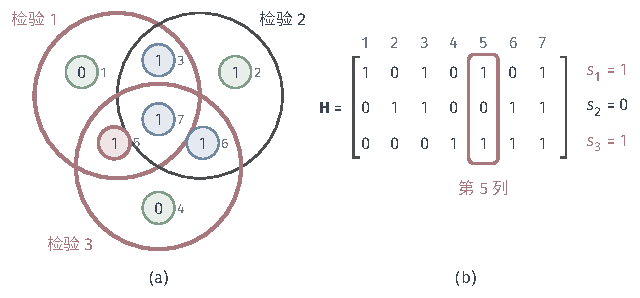
\includegraphics[width=108.3mm]{figures/07-probability/06-channel-coding/tikz/ccode-hamming-venn/figure.pdf}
 \caption{$[7,4,3]$ Hamming码的单错定位。(a) 三个圆是$\bm{H}_7$的三条校验，圆内比特之和应为偶数；小圆中的数是接收块$0110111$各位的值，旁边的小字是位置，绿色为校验位，蓝色为消息位，红色为被翻转的第$5$位。红色粗圆是不通过的检验。(b) 校验矩阵$\bm{H}_7$，第$j$列是$j$的二进制表示（自下而上读）；综合征$(s_1,s_2,s_3)=(1,0,1)$等于红框中的第$5$列。}
 \label{fig:ccode-hamming-venn}
\end{BookInlineFigure}

\paragraph{一个也不浪费}
半径为$1$的Hamming球含$1+7=8$个长度为$7$的串，$16$个码字的球互不相交，合计
\[
 16\times8=128=2^{7}
\]
个串，恰好铺满全部接收块。所以每个接收块都与唯一一条码字相距不超过$1$；$8$个综合征恰好对应“无错”和$7$个单错位置，没有一个综合征被浪费。代价也随之而来：两个翻转一定被“纠正”成第三个翻转。例如两位翻转$\bm{e}$的综合征是两列之和，它等于另一列，译码器会翻转那一位，结果与原码字相差三位。

\paragraph{与重复码对比}
Hamming码与三次重复码的最小距离都是$3$，都保证纠正一个翻转，但保证的范围不同。三次重复码在每$3$次使用中纠正一个翻转，每个消息比特各有自己的保护；Hamming码在$7$次使用中只纠正一个翻转，四个消息比特共享这份保护。前者码率$\tfrac13$，后者码率$\tfrac47\approx0.571$。

在$p=0.1$时，Hamming码的块错误概率是至少两位翻转的概率：
\[
 P_{\mathrm{e}}=1-0.9^7-7\times0.1\times0.9^6=1-0.47830-0.37201=0.14969 .
\]
三次重复码发送同样$4$个比特的块错误概率约为$0.107$，不编码时为$0.344$。逐个比特看，对$128$个错误向量逐一枚举综合征译码的结果，Hamming码的比特错误率是$0.0669$，三次重复码是$0.028$，不编码是$0.1$。

图~\ref{fig:ccode-hamming-ber}把比较延伸到不同的翻转概率。$p$较小时，两种码的比特错误率都与$p^2$同阶，因为都需要两个翻转才出错；Hamming码的系数更大，因为$7$位中出现两个翻转的方式比$3$位中多。$p=0.01$时，Hamming码的比特错误率为$8.7\times10^{-4}$，三次重复码为$3.0\times10^{-4}$。Hamming码用略高的错误换取了高得多的码率。

\begin{BookInlineFigure}
 \centering
 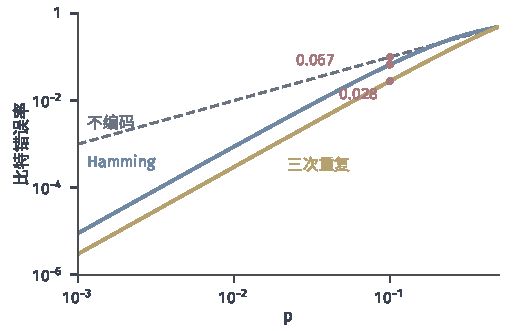
\includegraphics[width=88mm]{figures/07-probability/06-channel-coding/matplotlib/ccode-hamming-ber/figure.pdf}
 \caption{二元对称信道上的比特错误率随翻转概率$p$的变化，双对数坐标，均为精确值：不编码（灰色虚线，码率$1$），$[7,4,3]$ Hamming码配合综合征译码（蓝，码率$\tfrac47$，对$128$个错误向量逐一枚举），三次重复码配合多数判决（黄，码率$\tfrac13$）。红点为$p=0.1$处的值。}
 \label{fig:ccode-hamming-ber}
\end{BookInlineFigure}

\paragraph{有限构造不是容量的证明}
在$p=0.1$的信道上，Hamming码的码率$0.571$已经超过容量$0.531$。这并不矛盾：容量限制的是错误能否趋于零，单个有限码的错误概率$0.15$并不为零。同一族中更长的Hamming码码率更高，$r$个校验位对应码率
\[
 \frac{2^{r}-1-r}{2^{r}-1}\to1 ,
\]
但每个块只保证纠正一个翻转。块长$n$增大时，$n$个位置中至多一个翻转的概率$(1-p)^{n}+np(1-p)^{n-1}$趋于零，所以对固定的$p>0$，块错误概率趋于$1$。要让错误趋于零而码率保持为正，能纠正的翻转数必须随块长按比例增长，Hamming码族做不到这一点。它是一个结构清楚、译码极其简单的有限构造，不能当作渐近达到容量的例子。


\section{有限块的性能}
\label{sec:ccode-finite}

假设要在$p=0.1$的二元对称信道上设计一个块长$n=1000$的码，要求块错误概率不超过$10^{-3}$。码率最高能取多少？容量$0.531$只说码率低于它时，块长足够长就能把错误压到任意小，并不说$n=1000$够不够长，也不说需要多少冗余。本节固定信道、块长与错误口径，分三类陈述来回答：任何码都做不到的界限，某个码一定能做到的保证，以及具体码的实际数值。

\paragraph{评价的口径}
比较之前要先说清比较什么。第~\ref{chap:discrete-channel-capacity}章区分了平均错误概率与最大错误概率，本章又用到比特错误率，即消息比特被译错的平均比例。三者衡量不同的东西：Hamming码在$p=0.1$时块错误概率为$0.150$，比特错误率只有$0.067$，因为一个块出错时通常不是四个消息比特全错。下面说“错误概率”时指均匀消息下的平均块错误概率。对线性码配合综合征译码，各消息的条件错误概率相同，平均与最大两种口径一致。除错误以外，码率、冗余位数$n-k$以及编码与译码的计算量都是评价的一部分，它们之间需要权衡。

\paragraph{球填充界}
先看纯粹组合的限制。若一个码保证纠正$t$个翻转，即半径为$t$的判决球互不相交，那么$M$个球必须装进$2^{n}$个串里。半径为$t$的球所含串的个数是
\[
 V(n,t)=\sum_{j=0}^{t}\binom{n}{j} ,
\]
因为与中心相差恰好$j$位的串有$\binom nj$个，与中心无关。

\begin{theorem}[球填充界]
\label{thm:ccode-hamming-bound}
若长度为$n$的二元码本含$M$条码字，且以每条码字为中心、半径为$t$的Hamming球两两不相交，则
\begin{equation}
 M\,V(n,t)\leq2^{n},\qquad\text{即}\qquad R=\frac{\log_2M}{n}\leq1-\frac{\log_2V(n,t)}{n} .
 \label{eq:ccode-hamming-bound}
\end{equation}
\end{theorem}

\begin{proof}
$M$个两两不相交的球各含$V(n,t)$个串，它们的并集是$\{0,1\}^{n}$的子集，所以总数$MV(n,t)$不超过$2^{n}$。两边取以$2$为底的对数并除以$n$，得到码率的形式。
\end{proof}

由第~\ref{sec:ccode-min-distance}节，$d_{\min}\geq2t+1$的码满足定理的条件，所以式~\eqref{eq:ccode-hamming-bound}称为\term{球填充界}（sphere-packing bound），也叫Hamming界。等号成立时，球恰好铺满全部串，没有一个接收块落在球外，这样的码称为\term{完备码}（perfect code）。$t=1$时界为$M\leq2^{n}/(n+1)$。上一节的$[7,4,3]$码给出$16\times8=128$，是完备码；所有块长$n=2^{r}-1$的Hamming码都是完备码，因为
\[
 2^{\,n-r}(1+n)=2^{\,n-r}\cdot2^{r}=2^{n} .
\]
$[5,2,3]$码则有$4\times6=24<32$，剩下$8$个串不在任何球内，正是它在两个翻转上存在并列的原因。图~\ref{fig:ccode-hamming-bound}画出$t=1$时的界与这些码的位置。

\begin{BookInlineFigure}
 \centering
 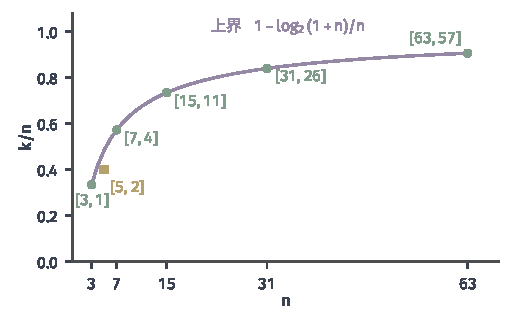
\includegraphics[width=88mm]{figures/07-probability/06-channel-coding/matplotlib/ccode-hamming-bound/figure.pdf}
 \caption{纠单错二元码的球填充界$k/n\leq1-\log_2(1+n)/n$（紫线，按整数$n$连成）。绿点是块长$n=2^{r}-1$的Hamming码，恰好落在界上；$[3,1]$即三次重复码。黄色方块是$[5,2,3]$码，位于界的下方。}
 \label{fig:ccode-hamming-bound}
\end{BookInlineFigure}

球填充界只依赖“保证纠正$t$个”这一组合要求，与信道的翻转概率无关。在$p=0.1$的信道上，块长$1000$时平均有$100$个翻转，若要求保证纠正它们，需要
\[
 R\leq1-\frac{\log_2V(1000,100)}{1000}\approx0.535 ,
\]
而且保证纠正$100$个并不够：翻转个数超过$100$的概率约为$0.47$。概率意义下的错误需要另外的论证。

\paragraph{错误概率的下界}
现在允许任意码本、任意解码器，只问块错误概率能小到什么程度。思路仍然是“领地”：解码器把每个接收块判给一条消息，于是$2^{n}$个接收块被分成$M$个判决区域$D_1,\dots,D_M$。消息$m$判对的概率是码字$\bm{c}_m$的输出落在$D_m$中的概率。一个区域能“接住”多少概率，取决于它包含哪些接收块；最划算的是包含离码字最近的那些，也就是一个Hamming球。

为了精确表述，把一条码字到全部$2^{n}$个接收块的转移概率从大到小排成
\[
 a_1\geq a_2\geq\cdots\geq a_{2^{n}} .
\]
在二元对称信道上，$W^{n}(\bm{y}\mid\bm{c})=p^{d}(1-p)^{n-d}$，其中$d=\operatorname{dist}(\bm{y},\bm{c})$；与码字相距$d$的接收块有$\binom nd$个，所以这个排列对每条码字都相同。定义
\begin{equation}
 g(s)=\sum_{i=1}^{\lfloor s\rfloor}a_i+(s-\lfloor s\rfloor)\,a_{\lfloor s\rfloor+1},\qquad 0\leq s\leq2^{n},
 \label{eq:ccode-g}
\end{equation}
约定$a_{2^{n}+1}=0$。整数$s$处，$g(s)$是最大的$s$个转移概率之和；整数之间线性插值。

\begin{theorem}[有限块长的逆向界]
\label{thm:ccode-sphere-converse}
在二元对称信道上，任意$M$条码字、块长为$n$的码，配合任意确定的解码器，均匀消息下的平均块错误概率满足
\begin{equation}
 1-P_{\mathrm{e}}\leq g\Bigl(\frac{2^{n}}{M}\Bigr) .
 \label{eq:ccode-sphere-converse}
\end{equation}
\end{theorem}

\begin{proof}
设判决区域为$D_1,\dots,D_M$，它们两两不相交，并集是全部$2^{n}$个接收块，所以
\[
 \sum_{m=1}^{M}\lvert D_m\rvert=2^{n} .
\]
均匀消息下判对的概率是
\[
 1-P_{\mathrm{e}}=\frac1M\sum_{m=1}^{M}\ \sum_{\bm{y}\in D_m}W^{n}(\bm{y}\mid\bm{c}_m) .
\]

第一步，固定$m$。$D_m$含$\lvert D_m\rvert$个接收块，它们的转移概率是$a_1,\dots,a_{2^{n}}$中的$\lvert D_m\rvert$个，和不超过最大的$\lvert D_m\rvert$个之和：
\[
 \sum_{\bm{y}\in D_m}W^{n}(\bm{y}\mid\bm{c}_m)\leq g(\lvert D_m\rvert) .
\]

第二步，$g$是凹函数。它在每个区间$[i-1,i]$上是斜率为$a_i$的线段，斜率随$i$不增，所以$g$是凹的。对有限个点取平均，凹函数满足Jensen不等式：
\[
 \frac1M\sum_{m=1}^{M}g(\lvert D_m\rvert)\leq g\Bigl(\frac1M\sum_{m=1}^{M}\lvert D_m\rvert\Bigr)=g\Bigl(\frac{2^{n}}{M}\Bigr) .
\]
两步合起来就是式~\eqref{eq:ccode-sphere-converse}。
\end{proof}

这个界的读法是：最理想的情形是每条码字恰好独占一个大小为$2^{n}/M$、由离它最近的接收块组成的区域。码字越多，每条分到的区域越小，能接住的概率越少。证明中两个不等号同时取等，要求每个判决区域都是以码字为中心的Hamming球（必要时连同一部分下一层），且大小都相同。完备码满足这一点。

对$n=7$、$M=16$，$2^{7}/16=8$，最大的$8$个转移概率是距离$0$的一个与距离$1$的七个，于是
\[
 1-P_{\mathrm{e}}\leq0.9^7+7\times0.1\times0.9^6=0.85031 .
\]
上一节算出Hamming码的块错误概率恰好是$0.14969$，等号成立。所以在$p=0.1$的二元对称信道上，没有任何$16$条码字、块长为$7$的码，配合任何解码器，能比$[7,4,3]$ Hamming码做得更好。

同样的计算也适用于重复码。块长$7$、两条码字时$2^{7}/2=64$，而半径为$3$的球恰含
\[
 V(7,3)=1+7+21+35=64
\]
个串，所以
\[
 1-P_{\mathrm{e}}\leq\mathbb{P}(\text{翻转个数}\leq3)=0.997272 .
\]
七次重复码的错误概率是$0.002728$，又一次取到等号：长度为奇数$n=2t+1$的重复码也是完备码，它的两个半径为$t$的球恰好平分全部$2^{n}$个串。于是在$p=0.1$的信道上，块长为$7$的码即使只传一个比特，错误概率也不可能低于$0.0027$，要求$10^{-3}$就必须加长块。

反过来，给定目标错误$\varepsilon$，式~\eqref{eq:ccode-sphere-converse}限制了码字个数。$g$单调增，设$s^{*}$是使$g(s)\geq1-\varepsilon$的最小$s$，则任何满足$P_{\mathrm{e}}\leq\varepsilon$的码都有$2^{n}/M\geq s^{*}$，即
\begin{equation}
 R\leq1-\frac{\log_2s^{*}}{n} .
 \label{eq:ccode-converse-rate}
\end{equation}
$s^{*}$可以按距离由近到远累加$\binom nd p^{d}(1-p)^{n-d}$精确算出。

\paragraph{随机码的保证}
另一个方向要证明某个码确实能做到。第~\ref{chap:discrete-channel-capacity}章用随机码本证明了可达性，那里的估计是为渐近目的设计的；在二元对称信道上，同样的思路可以给出一个对每个$n$都能精确计算的界，称为\term{随机编码并集界}。

\begin{theorem}[随机编码并集界]
\label{thm:ccode-rcu}
在翻转概率$p<\tfrac12$的二元对称信道上，对任意块长$n$与码字个数$M\geq1$，存在一个码本，配合最小距离译码，其平均块错误概率满足
\begin{equation}
 P_{\mathrm{e}}\leq\sum_{k=0}^{n}\binom nk p^{k}(1-p)^{n-k}\min\Bigl\{1,\ (M-1)\,\frac{V(n,k)}{2^{n}}\Bigr\} .
 \label{eq:ccode-rcu}
\end{equation}
\end{theorem}

\begin{proof}
独立地从$\{0,1\}^{n}$中均匀抽取$M$条码字。解码器选距离最近的码字，并且只要有别的码字与接收块的距离不超过正确码字，就把这次传输算作错误；这只会高估错误。

固定消息$m$，设信道翻转了$k$位，接收块为$\bm{y}$，于是$\operatorname{dist}(\bm{y},\bm{c}_m)=k$。判错要求某个$j\neq m$满足$\operatorname{dist}(\bm{c}_j,\bm{y})\leq k$。$\bm{c}_j$与$\bm{c}_m$、与信道噪声都独立，并且在$\{0,1\}^{n}$上均匀，所以对每个固定的$\bm{y}$，
\[
 \mathbb{P}\bigl(\operatorname{dist}(\bm{c}_j,\bm{y})\leq k\bigr)=\frac{V(n,k)}{2^{n}} .
\]
对$M-1$个竞争者用并集上界，再与$1$取小，得到在给定$k$时判错的条件概率不超过
\[
 \min\Bigl\{1,\ (M-1)\,\frac{V(n,k)}{2^{n}}\Bigr\} .
\]
翻转个数$k$服从$\operatorname{Bin}(n,p)$，对$k$取平均，得到对码本与噪声一起取期望后，消息$m$的错误概率不超过式~\eqref{eq:ccode-rcu}右边。这个界对每个$m$相同，所以随机码本的平均错误概率的期望也不超过它；一个随机变量不可能处处大于自己的均值，于是某个具体码本的平均错误概率不超过它。
\end{proof}

右边的$\min$体现了两种错误来源的分工。翻转少时，$V(n,k)/2^{n}$极小，竞争码字几乎不可能靠得更近；翻转多到使$(M-1)V(n,k)\geq2^{n}$时，球内平均已有一个以上的竞争者，这时直接按判错计算。这正是第~\ref{chap:discrete-channel-capacity}章典型性论证的有限块版本。

\paragraph{两条界之间}
对给定的$n$与目标错误$\varepsilon$，用二分法求出使式~\eqref{eq:ccode-rcu}右边不超过$\varepsilon$的最大$\log_2M$，就得到随机码能保证的码率；式~\eqref{eq:ccode-converse-rate}给出任何码都不能超过的码率。真正最优的码率夹在两者之间。图~\ref{fig:ccode-finite-rate}在$p=0.1$、$\varepsilon=10^{-3}$下画出这两条曲线。

\begin{BookInlineFigure}
 \centering
 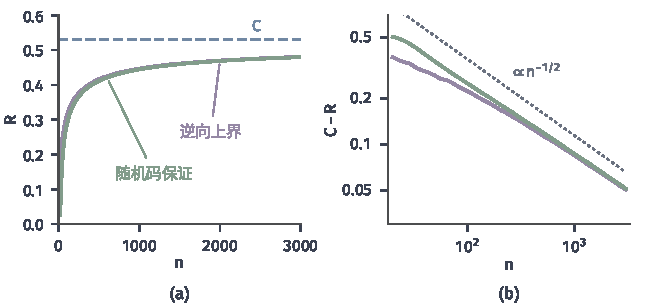
\includegraphics[width=110mm]{figures/07-probability/06-channel-coding/matplotlib/ccode-finite-rate/figure.pdf}
 \caption{$p=0.1$的二元对称信道上，平均块错误概率不超过$10^{-3}$时的码率界限，均为精确计算。紫线为式~\eqref{eq:ccode-converse-rate}的逆向上界，任何码都在它下方；绿线为由式~\eqref{eq:ccode-rcu}得到的随机码保证，存在码达到它；蓝色虚线为容量$C=0.531$。(a) 码率随块长$n$的变化，两条曲线几乎重合；(b) 两者与容量的差$C-R$，双对数坐标，灰色点线是斜率$-\tfrac12$的参照。}
 \label{fig:ccode-finite-rate}
\end{BookInlineFigure}

从图中读出几组数：$n=100$时，最优码率在$0.281$与$0.309$之间；$n=1000$时，在$0.444$与$0.447$之间。容量是$0.531$，所以开头的问题有了确定的答案：块长$1000$、错误不超过$10^{-3}$，码率至多约$0.447$，比容量低约$16\%$；也就是说，冗余至少要占$55\%$，而容量只要求约$47\%$。图(b)显示，两条界与容量之差都大致按$n^{-1/2}$缩小。这是对这两条界的数值观察，直观上来自翻转个数$\operatorname{Bin}(n,p)$的波动：它的标准差是$\sqrt{np(1-p)}$，为了以$1-\varepsilon$的概率覆盖这些波动，每个码字的领地要比“平均翻转个数”多留出与$\sqrt n$同阶的余量，摊到每个符号上就是$n^{-1/2}$。把这一直观变成关于最优码率的定理，需要对中心极限定理的误差作定量控制，本章不作证明。

\paragraph{计算的代价}
两条界都只关心错误概率，没有计入编码与译码的成本。随机码保证的码在$n=1000$、$R=0.444$时有$2^{444}$条码字，既无法存储，也无法逐一比较。即使改用线性码，综合征对照表也有$2^{556}$项。下面的表把本章出现的几种做法放在一起。

\begin{BookInlineTable}
 \centering
 \caption{有限块编码的码率、错误与计算代价（二元对称信道，$p=0.1$）}
 \label{tab:ccode-cost}
 \begin{tabular}{lllll}
 \toprule
 方案 & 码率 & 块错误 & 存储 & 每块译码运算 \\
 \midrule
 三次重复 & $1/3$ & $0.028$ & 无 & $3$次 \\
 $[5,2,3]$线性码 & $0.4$ & $0.067$ & $8$项表 & $15$次 \\
 $[7,4,3]$ Hamming & $4/7$ & $0.150$ & 无 & $21$次 \\
 $[n,k]$线性码 & $k/n$ & 依码而定 & $2^{n-k}$项表 & $(n-k)n$次 \\
 随机码本 & $\log_2M/n$ & 式~\eqref{eq:ccode-rcu} & $Mn$比特 & $Mn$次 \\
 \bottomrule
 \end{tabular}
\end{BookInlineTable}

表中的“每块译码运算”只计多数判决、综合征或逐一比较所需的比特运算，不计查表与读写；$[n,k]$线性码一行假设对照表已经存在，建表本身要枚举错误向量。块错误概率一列中，重复码和$[5,2,3]$码针对的消息比特数不同，比较时要换算到相同的消息长度，如第~\ref{sec:ccode-syndrome}小节所做。

\paragraph{三类陈述}
本节的结论可以归为三类，它们回答不同的问题。
\begin{itemize}
 \item 理论下界：球填充界与逆向界~\eqref{eq:ccode-sphere-converse}对所有码、所有解码器成立，说明“不可能更好”，但不提供任何码。
 \item 构造保证：随机编码并集界说明“存在至少这样好的码”，同时只给出一个需要指数级存储与搜索的码，不说明怎样找到便宜的码。
 \item 实际计算：重复码、$[5,2,3]$码与Hamming码的错误概率是对具体码和具体译码器的精确计算，它们落在界的哪一侧、离界多远，才说明这个构造好不好。
\end{itemize}
容量是这几类陈述在块长趋于无穷时的共同极限。它约束了渐近可达的速率，单凭它不能回答给定块长需要多少冗余，也不能回答需要多大的计算量。


\section{信源信道分离}
\label{sec:ccode-separation}

到目前为止，信道上传送的都是等可能的消息比特。实际要传的消息来自一个信源：例如每天记录一次“是否下雨”，下雨的概率是$0.1$。这样的比特高度可预测，第~\ref{chap:lossless-coding}章说明它们平均每个只含$h_2(0.1)\approx0.469$比特信息。现在要通过$p=0.1$的二元对称信道传送它们。一种做法是先压缩、再加冗余；另一种做法是把压缩与纠错合在一起设计。分开做会不会损失什么？

\paragraph{计量的统一}
信源编码按“每个源符号多少比特”计量，信道编码按“每次信道使用多少比特”计量。把两者接起来，需要规定源符号与信道使用的比例。设信源依次产生$S_1,S_2,\dots$，相互独立，都服从有限字母表$\mathcal{S}$上的分布$P_S$；信道是有限字母表上的离散无记忆信道，容量为$C$，编码器不使用反馈。

一个块长为$(k,n)$的\term{联合信源信道编码}（joint source-channel coding）由两个映射组成：编码器把$k$个源符号映成$n$个信道输入，
\[
 f:\mathcal{S}^{k}\to\mathcal{X}^{n},
\]
解码器把$n$个信道输出映成$k$个重构符号，
\[
 g:\mathcal{Y}^{n}\to\hat{\mathcal{S}}^{k} .
\]
考虑一列这样的码，块长$n\to\infty$，并且
\begin{equation}
 \frac{k_n}{n}\to r>0 .
 \label{eq:ccode-ratio}
\end{equation}
$r$是每次信道使用平均传送的源符号个数。它把两种计量统一起来：信源每个符号需要$H$比特时，每次信道使用就需要承载$rH$比特，这个量才能与容量比较。$r>0$保证$k_n$也趋于无穷，两边的块长同时增长。

\paragraph{分离的构造}
分离方案中，编码器分两步：先用信源编码把$S^{k}$映成一个编号$m$，再用信道编码把编号映成码字$X^{n}$；解码器反过来，先由信道输出判出编号$\hat{m}$，再由编号重构源块。图~\ref{fig:ccode-separation-pipeline}画出这条链路。两个编码器之间只传递一个编号，彼此不需要知道对方的细节：信源编码不关心信道的转移概率，信道编码不关心编号的含义。

\begin{BookInlineFigure}
 \centering
 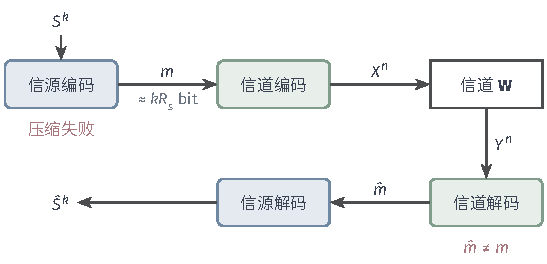
\includegraphics[width=92.7mm]{figures/07-probability/06-channel-coding/tikz/ccode-separation-pipeline/figure.pdf}
 \caption{分离的信源信道传输。$k$个源符号$S^{k}$经信源编码（蓝）变成编号$m$，约用$kR_{\mathrm{s}}$比特描述；信道编码（绿）把编号映成$n$个信道输入，经信道$\bm{W}$得到输出，信道解码给出编号的判决$\hat{m}$，信源解码给出重构$\hat{S}^{k}$。红字标出两种失败：信源编码本身失败，以及编号被判错。}
 \label{fig:ccode-separation-pipeline}
\end{BookInlineFigure}

下面先在无损要求下、再在失真要求下说明这一构造何时可行，以及任何方案（不论是否分离）都必须满足什么条件。若信道输入有逐码字的成本预算，第~\ref{chap:discrete-channel-capacity}章给出的受限容量与满足预算的码可以照样代入，下文的$C$换成对应的受限容量。

\subsection{无损传输}
\label{sec:ccode-lossless-transmission}

无损的要求是整块源符号被正确恢复的概率趋于$1$，此时$\hat{\mathcal{S}}=\mathcal{S}$。以下熵$H(S)$都以bit计。

\begin{theorem}[无损传输的分离定理]
\label{thm:ccode-lossless-separation}
设信源与信道如上，比例$r$满足式~\eqref{eq:ccode-ratio}。
\begin{enumerate}
 \item 若$rH(S)<C$，则存在一列分离方案，使
 \begin{equation}
  \mathbb{P}\bigl(\hat{S}^{k_n}\neq S^{k_n}\bigr)\to0 .
  \label{eq:ccode-lossless-goal}
 \end{equation}
 \item 若某一列联合信源信道编码（不必分离）满足式~\eqref{eq:ccode-lossless-goal}，则
 \begin{equation}
  rH(S)\leq C .
  \label{eq:ccode-lossless-converse}
 \end{equation}
\end{enumerate}
\end{theorem}

\paragraph{可达性的证明}
思路是在压缩与传输之间各留一点速率余量。因为$rH(S)<C$，可以选两个数$R_{\mathrm{s}}$与$R_{\mathrm{c}}$，使
\[
 H(S)<R_{\mathrm{s}},\qquad rR_{\mathrm{s}}<R_{\mathrm{c}}<C .
\]
先取$R_{\mathrm{s}}$略大于$H(S)$且$rR_{\mathrm{s}}<C$，再在$rR_{\mathrm{s}}$与$C$之间取$R_{\mathrm{c}}$。$R_{\mathrm{s}}$是信源编码的码率（每源符号的比特数），$R_{\mathrm{c}}$是信道编码的码率（每次使用的比特数）。

信源一侧，第~\ref{chap:lossless-coding}章的定长块编码可达性给出：对$R_{\mathrm{s}}>H(S)$，存在把$S^{k}$映成至多$2^{kR_{\mathrm{s}}}$个编号的定长编码，使不能正确还原的概率$\delta_k\to0$。信道一侧，第~\ref{chap:discrete-channel-capacity}章的编码定理给出：对$R_{\mathrm{c}}<C$，存在至少$2^{nR_{\mathrm{c}}}$条消息、最大错误概率$\lambda_{\max}^{(n)}\to0$的码。

两侧要能接上，编号的个数不能超过信道码的消息数。由$k_n/n\to r$与$rR_{\mathrm{s}}<R_{\mathrm{c}}$，$n$充分大时
\[
 k_nR_{\mathrm{s}}\leq nR_{\mathrm{c}} ,
\]
于是$2^{k_nR_{\mathrm{s}}}\leq2^{nR_{\mathrm{c}}}$。只使用信道码的前一部分消息即可；去掉的消息原来的判决区域可以并入任意保留的消息，保留消息的判决区域只增不减，所以最大错误概率不会变大。

整块恢复失败，只可能是信源编码失败或编号被判错，用并集上界：
\[
 \mathbb{P}\bigl(\hat{S}^{k}\neq S^{k}\bigr)\leq\delta_{k}+\mathbb{P}(\hat{m}\neq m) .
\]
信道噪声与信源独立，给定编号为$m$时判错的条件概率就是信道码的$\lambda_m$。编号的分布由信源决定，一般很不均匀，但无论它怎样分布，
\[
 \mathbb{P}(\hat{m}\neq m)=\sum_{m}\mathbb{P}(\text{编号}=m)\,\lambda_m\leq\lambda_{\max}^{(n)} .
\]
两项都趋于零，式~\eqref{eq:ccode-lossless-goal}成立。

这一步解释了为什么需要第~\ref{chap:discrete-channel-capacity}章的最大错误概率。若只知道均匀消息下的平均错误小，个别消息可能错误很大；而压缩后的编号恰好可能集中在这些消息上。逐消息的保证使信道码对任何编号分布都可靠。第~\ref{chap:discrete-channel-capacity}章删除坏码字的例子中，一个$16$条码字的随机码平均错误为$0.069$，最差的一条消息却达到$0.253$；若压缩后的编号恰好常常落在这条消息上，实际错误就接近$0.253$而不是$0.069$。

\paragraph{逆定理的证明}
现在设任一列联合编码满足式~\eqref{eq:ccode-lossless-goal}，把整块恢复失败的概率记作$P_{\mathrm{e}}^{(n)}$。信源无记忆，块的熵是单个熵的$k$倍，按熵与互信息的关系，
\[
 kH(S)=H(S^{k})=H(S^{k}\mid\hat{S}^{k})+I(S^{k};\hat{S}^{k}) .
\]

第一项用第~\ref{chap:information-measures}章的Fano不等式。$S^{k}$至多取$\lvert\mathcal{S}\rvert^{k}$个值，以bit计，
\[
 H(S^{k}\mid\hat{S}^{k})\leq1+P_{\mathrm{e}}^{(n)}\,k\log_2\lvert\mathcal{S}\rvert .
\]

第二项用数据处理不等式。编码器只看$S^{k}$，没有反馈，给定$X^{n}$后$Y^{n}$的条件分布不再依赖$S^{k}$，解码器只看$Y^{n}$，所以$S^{k}$、$X^{n}$、$Y^{n}$、$\hat{S}^{k}$按顺序构成Markov链。再用第~\ref{chap:discrete-channel-capacity}章的块互信息上界，
\[
 I(S^{k};\hat{S}^{k})\leq I(X^{n};Y^{n})\leq nC .
\]

两项相加，得到
\[
 kH(S)\leq1+P_{\mathrm{e}}^{(n)}\,k\log_2\lvert\mathcal{S}\rvert+nC .
\]
两边除以$n$，
\[
 \frac{k_n}{n}H(S)\leq\frac1n+P_{\mathrm{e}}^{(n)}\,\frac{k_n}{n}\log_2\lvert\mathcal{S}\rvert+C .
\]
令$n\to\infty$，$k_n/n\to r$，$P_{\mathrm{e}}^{(n)}\to0$，就得到式~\eqref{eq:ccode-lossless-converse}。

逆定理没有假设编码是分离的，它对任何把信源和信道合在一起的设计都成立。所以在$rH(S)\neq C$的地方，分离方案与最好的联合方案有相同的可行范围：分离在渐近意义下不损失任何速率。

\paragraph{例子}
回到开头的雨天记录，$P_S=\operatorname{Bern}(0.1)$，信道是$p=0.1$的二元对称信道：
\[
 H(S)=h_2(0.1)\approx0.469,\qquad C=1-h_2(0.1)\approx0.531 .
\]
定理给出的界限是
\[
 r<\frac{C}{H(S)}\approx1.13 .
\]
也就是说，每次信道使用可以可靠地传送约$1.13$个源比特，多于一个。不压缩而直接把源比特当作消息比特送进信道码，只能做到$r<C=0.531$。特别地，$r=1$时$rH(S)=0.469<0.531$，可以让每次信道使用传送一个源比特而几乎不出错；直接发送则有$10\%$的比特出错。图~\ref{fig:ccode-lossless-budget}画出不同信源参数下的界限：信源越可预测，压缩带来的收益越大。

\begin{BookInlineFigure}
 \centering
 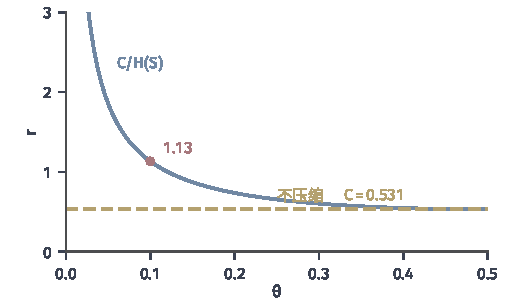
\includegraphics[width=86mm]{figures/07-probability/06-channel-coding/matplotlib/ccode-lossless-budget/figure.pdf}
 \caption{$\operatorname{Bern}(\theta)$信源经$p=0.1$的二元对称信道无损传输时，每次信道使用可传送的源符号数$r$的上限。蓝线为$C/H(S)=C/h_2(\theta)$，红点为$\theta=0.1$时的$1.13$；黄色虚线为不压缩时的上限$C=0.531$。$\theta=\tfrac12$时信源已无冗余，两者相等。}
 \label{fig:ccode-lossless-budget}
\end{BookInlineFigure}

\subsection{有损传输}
\label{sec:ccode-lossy-transmission}

许多信源不必精确恢复，只要重构的平均失真不超过某个水平。这时信源一侧用第~\ref{chap:rate-distortion}章的率失真编码代替无损压缩。

\paragraph{设定}
设重构字母表$\hat{\mathcal{S}}$有限，失真函数有界：
\[
 d:\mathcal{S}\times\hat{\mathcal{S}}\to[0,d_{\max}] .
\]
块的失真取逐符号平均
\[
 d_k(s^{k},\hat{s}^{k})=\frac1k\sum_{i=1}^{k}d(s_i,\hat{s}_i) .
\]
要求是渐近期望失真不超过$D$：
\begin{equation}
 \limsup_{n\to\infty}\mathbb{E}\bigl[d_{k_n}(S^{k_n},\hat{S}^{k_n})\bigr]\leq D .
 \label{eq:ccode-lossy-goal}
\end{equation}
这里的$R(D)$是第~\ref{chap:rate-distortion}章的信息率失真函数：在满足$\mathbb{E}\,d(S,\hat{S})\leq D$的测试信道中，互信息$I(S;\hat{S})$的下确界。那里证明了它非增、凸，在取有限值的区间上连续，并且等于渐近期望失真下的最低描述率。

\begin{theorem}[有损传输的分离定理]
\label{thm:ccode-lossy-separation}
在上述设定下：
\begin{enumerate}
 \item 若$rR(D)<C$，则存在一列分离方案满足式~\eqref{eq:ccode-lossy-goal}。
 \item 若某一列联合信源信道编码满足式~\eqref{eq:ccode-lossy-goal}，则
 \begin{equation}
  rR(D)\leq C .
  \label{eq:ccode-lossy-converse}
 \end{equation}
\end{enumerate}
\end{theorem}

\paragraph{可达性的证明}
与无损情形一样留出余量：取$R_{\mathrm{s}}'>R_{\mathrm{s}}>R(D)$与$R_{\mathrm{c}}$，使
\[
 rR_{\mathrm{s}}'<R_{\mathrm{c}}<C .
\]
由第~\ref{chap:rate-distortion}章的率失真编码定理，$(R_{\mathrm{s}},D)$是可达码率失真对：存在一列率失真码，码率的上极限不超过$R_{\mathrm{s}}$，期望失真的上极限不超过$D$。于是$k$充分大时，编号个数$M_k\leq2^{kR_{\mathrm{s}}'}$。信道一侧与无损情形相同，取最大错误概率$\lambda_{\max}^{(n)}\to0$的信道码，$n$充分大时编号能够放进去。

失真按两种情形分开估计。编号被正确判出时，重构就是率失真码本身的重构，失真与不经过信道时相同；编号被判错时，重构是另一条码字，失真不超过$d_{\max}$。所以
\[
 \mathbb{E}\bigl[d_k(S^{k},\hat{S}^{k})\bigr]\leq\mathbb{E}\bigl[d_k\bigl(S^{k},g_k(f_k(S^{k}))\bigr)\bigr]+d_{\max}\,\lambda_{\max}^{(n)} ,
\]
其中$f_k,g_k$是率失真码的编码与重构。第一项的上极限不超过$D$，第二项趋于零，式~\eqref{eq:ccode-lossy-goal}成立。有界失真在这里起关键作用：信道偶尔出错时，造成的额外失真被$d_{\max}$乘以一个趋于零的概率控制住。

\paragraph{逆定理的证明}
设$D_k=\mathbb{E}[d_k(S^{k},\hat{S}^{k})]$，$D_{k,i}=\mathbb{E}[d(S_i,\hat{S}_i)]$，于是$D_k$是$D_{k,i}$对$i$的平均。先给互信息一个下界。由链式法则与源符号的独立性，
\[
 I(S^{k};\hat{S}^{k})=H(S^{k})-H(S^{k}\mid\hat{S}^{k})=\sum_{i=1}^{k}H(S_i)-H(S^{k}\mid\hat{S}^{k}) .
\]
条件熵满足次可加性，并且多加条件不会增加熵，所以
\[
 H(S^{k}\mid\hat{S}^{k})\leq\sum_{i=1}^{k}H(S_i\mid\hat{S}^{k})\leq\sum_{i=1}^{k}H(S_i\mid\hat{S}_i) .
\]
代回，得到
\[
 I(S^{k};\hat{S}^{k})\geq\sum_{i=1}^{k}I(S_i;\hat{S}_i) .
\]

每一对$(S_i,\hat{S}_i)$的联合分布中，$S_i\sim P_S$，给定$S_i$时$\hat{S}_i$的条件分布是一个平均失真为$D_{k,i}$的测试信道，所以$I(S_i;\hat{S}_i)\geq R(D_{k,i})$。再由$R$的凸性（Jensen不等式），
\[
 \sum_{i=1}^{k}R(D_{k,i})\geq kR\Bigl(\frac1k\sum_{i=1}^{k}D_{k,i}\Bigr)=kR(D_k) .
\]
另一方面，与无损情形相同的Markov链与块互信息上界给出$I(S^{k};\hat{S}^{k})\leq nC$。合起来，
\[
 \frac{k_n}{n}\,R(D_{k_n})\leq C .
\]

最后取极限。任取$\eta>0$，由式~\eqref{eq:ccode-lossy-goal}，$n$充分大时$D_{k_n}\leq D+\eta$；$R$非增，所以
\[
 R(D+\eta)\leq R(D_{k_n})\leq\frac{n}{k_n}C\to\frac Cr .
\]
于是对每个$\eta>0$都有$rR(D+\eta)\leq C$。若$D$低于最小可行失真$D_{\min}$，任何重构都有$D_k\geq D_{\min}$，式~\eqref{eq:ccode-lossy-goal}不可能成立，所以只需考虑$D\geq D_{\min}$，此时$R(D)$有限。第~\ref{chap:rate-distortion}章证明了$R$在$[D_{\min},\infty)$上连续（包括左端点），令$\eta\downarrow0$，就得到式~\eqref{eq:ccode-lossy-converse}。

\paragraph{例子：均匀二元信源}
设$P_S=\operatorname{Bern}(\tfrac12)$，Hamming失真，信道仍是$p=0.1$的二元对称信道。由第~\ref{chap:rate-distortion}章，
\[
 R(D)=1-h_2(D),\qquad 0\leq D\leq\tfrac12 .
\]
给定$r$，能达到的最小失真$D^{*}(r)$由$rR(D)=C$决定：$r\leq C$时任何正失真都可以达到（无损传输的条件$rH(S)=r<C$在$r<C$时就已满足）；$r>C$时
\begin{equation}
 D^{*}(r)=h_2^{-1}\Bigl(1-\frac Cr\Bigr) ,
 \label{eq:ccode-dstar}
\end{equation}
其中$h_2^{-1}$是$h_2$在$[0,\tfrac12]$上的反函数。$r=1$时$1-C=h_2(0.1)$，所以
\[
 D^{*}(1)=0.1 .
\]
$r=2$时$1-C/2\approx0.735$，$D^{*}(2)\approx0.206$。

图~\ref{fig:ccode-lossy-tradeoff}把这条曲线与几个具体方案放在一起。三次与五次重复码的$r$分别为$\tfrac13$与$\tfrac15$，每个源比特的错误率是$0.028$与$0.0086$，而在这些$r$上理论上可以把失真压到任意小。Hamming码在$r=\tfrac47$处的比特错误率是$0.067$，界限是$0.0085$。$r=2$时，“发送一个比特、另一个猜”的失真是$(0.1+0.5)/2=0.3$，界限是$0.206$。最引人注意的是$r=1$：把源比特原样送进信道，不做任何编码，失真正好是$0.1$，恰好落在界限上。

\begin{BookInlineFigure}
 \centering
 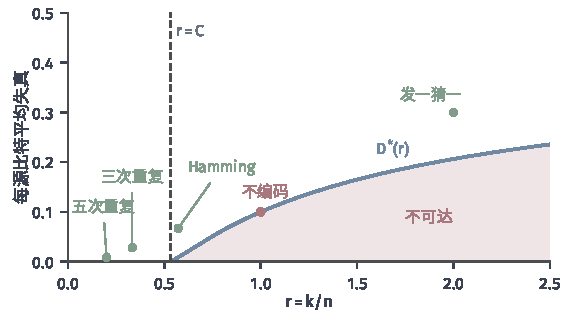
\includegraphics[width=96mm]{figures/07-probability/06-channel-coding/matplotlib/ccode-lossy-tradeoff/figure.pdf}
 \caption{均匀二元信源、Hamming失真、$p=0.1$的二元对称信道。蓝线为式~\eqref{eq:ccode-dstar}的最小可达失真$D^{*}(r)$（$r\leq C$时为$0$），其下方的红色区域被逆定理排除；虚线为$r=C$。绿点为具体方案的精确值：五次重复、三次重复、$[7,4,3]$ Hamming码的比特错误率，以及$r=2$时发一个比特、猜另一个。红点为不编码直接发送，$r=1$，失真$0.1$。}
 \label{fig:ccode-lossy-tradeoff}
\end{BookInlineFigure}

\subsection{分离原则的范围}
\label{sec:ccode-separation-scope}

两条分离定理说：在规定的条件下，比较$rH(S)$或$rR(D)$与$C$这两个数，就决定了传输能否成功，并且分开设计足以达到这个界限。这个结论的每一部分都附带条件，去掉条件，结论就可能失效或需要另行论证。

\paragraph{严格不等式与渐近}
可达性需要严格不等式$rR(D)<C$，因为证明要在压缩与传输两侧各留一点余量；逆定理只给出非严格的$rR(D)\leq C$。在等号$rR(D)=C$处，定理既不保证可以做到，也不保证做不到。而且两边都是块长趋于无穷的陈述：它们不承诺某个有限的块长已经足够，不承诺零错误，也不承诺失真恰好等于$D$。第~\ref{sec:ccode-finite}节已经看到，单是信道一侧，块长$1000$就要比容量多付出约$16\%$的码率；分离方案在信源一侧还有另一份有限块的损失。

\paragraph{联合方案可以更简单}
上面均匀二元信源的例子中，不编码直接发送在$k=n=1$、没有任何延迟的情况下就达到了$D^{*}(1)=0.1$；分离方案要接近同一失真，两侧的块长都必须很长。原因是这个信源与信道恰好“匹配”：均匀的源比特正是使二元对称信道达到容量的输入分布，信道的翻转又恰好产生信源所需的Hamming失真。分离定理说分开设计不吃亏，不是说分开设计是唯一的好办法；在有限延迟下，匹配的联合方案可以严格优于有限块长的分离方案。

\paragraph{高斯信源与无界失真}
同样的匹配也出现在连续的情形。设信源$S\sim\mathcal{N}(0,\sigma_S^{2})$，信道是$Y=X+Z$，$Z\sim\mathcal{N}(0,\sigma_Z^{2})$与输入独立，输入功率不超过$P_{\mathrm{s}}$（这里用$P_{\mathrm{s}}$表示功率，以免与概率混淆）。每次使用传送一个源符号，即$r=1$。

不编码时发送$X=aS$，其中$a=\sqrt{P_{\mathrm{s}}/\sigma_S^{2}}$使功率恰为$P_{\mathrm{s}}$，接收端用$\mathbb{E}[S\mid Y]$估计$S$。$(S,Y)$是联合高斯的，$\operatorname{Cov}(S,Y)=a\sigma_S^{2}$，$\operatorname{Var}(Y)=P_{\mathrm{s}}+\sigma_Z^{2}$，最优估计$\mathbb{E}[S\mid Y]$是$Y$的线性函数，它的均方误差是条件方差：
\[
 \begin{aligned}
 \operatorname{Var}(S\mid Y)&=\sigma_S^{2}-\frac{\operatorname{Cov}(S,Y)^{2}}{\operatorname{Var}(Y)}=\sigma_S^{2}-\frac{a^{2}\sigma_S^{4}}{P_{\mathrm{s}}+\sigma_Z^{2}}\\
 &=\sigma_S^{2}-\frac{P_{\mathrm{s}}\sigma_S^{2}}{P_{\mathrm{s}}+\sigma_Z^{2}}=\frac{\sigma_S^{2}\sigma_Z^{2}}{P_{\mathrm{s}}+\sigma_Z^{2}} .
 \end{aligned}
\]

另一方面，第~\ref{chap:rate-distortion}章的高斯率失真函数与第~\ref{chap:gaussian-channel-capacity}章的高斯信道容量给出$r=1$时的界限
\[
 \frac12\log_2\frac{\sigma_S^{2}}{D}\leq\frac12\log_2\Bigl(1+\frac{P_{\mathrm{s}}}{\sigma_Z^{2}}\Bigr) ,
\]
即
\[
 D\geq\frac{\sigma_S^{2}\sigma_Z^{2}}{P_{\mathrm{s}}+\sigma_Z^{2}} .
\]
不编码再次恰好达到界限。

但这里的分离定理不能照搬上面的证明。平方失真$(s-\hat{s})^{2}$无界，可达性证明中“信道出错时失真不超过$d_{\max}$”这一步失效：编号被判错时，重构可能离信源很远，额外的失真不再被一个趋于零的概率乘以常数所控制。要沿用分离构造，必须另外控制信道出错事件上的失真，例如限制重构值的范围并利用信源的二阶矩证明这部分期望趋于零。字母表也不再有限，率失真编码与信道编码本身都要用连续情形的定理。

\paragraph{记忆与有限延迟}
本节的信源与信道都是无记忆的，块长可以任意增长。若信源相邻符号相关，或信道的噪声随时间相关，熵和容量都要换成按单位时间计算的极限量，这些极限是否存在、是否等于可操作的速率，取决于过程的平稳性与遍历性一类条件，需要随机过程的工具另行建立。若应用要求有限延迟，块长不能任意增长，就需要直接核算有限块的代价。在这些情形下，只比较两个标量速率并沿用全部结论是不够的。


\section{本章小结}
\label{sec:ccode-summary}

本章从容量的存在性结论转向具体的码：在$p=0.1$的二元对称信道上，用有限的块长与可以执行的判决规则纠正翻转，并把信源压缩接到信道传输之前。开头的问题有了答案：$[7,4,3]$ Hamming码只用$7$次信道发送$4$个比特，任意一个翻转都能由综合征直接定位并改正。

\paragraph{主要结论}
\begin{itemize}
 \item 冗余与距离：长度为$2t+1$的重复码在多数判决下恰好纠正至多$t$个翻转，块错误概率由二项分布的尾部给出。一般码本的纠错能力由最小距离$d_{\min}$刻画：保证检测$d_{\min}-1$个翻转，在最小距离译码下保证纠正$\lfloor(d_{\min}-1)/2\rfloor$个翻转，保证来自互不相交的判决球；超出半径后的错误要按具体信道与并列规则计算。

 \item 线性结构：$[n,k]$二元线性码是$\mathbb{F}_2^{n}$的$k$维子空间，最小距离等于最小非零重量。生成矩阵$\bm{G}$把编码变成$\bm{c}=\bm{u}\bm{G}$，存储从$2^{k}n$比特降到$kn$比特；校验矩阵$\bm{H}$满足$\bm{G}\bm{H}^{\top}=\bm{0}$，综合征$\bm{H}\bm{y}^{\top}=\bm{H}\bm{e}^{\top}$只依赖错误。综合征译码选取陪集中重量最小的错误，在二元对称信道上就是最大似然解码；它判对当且仅当真实错误恰为陪集首，但对照表有$2^{n-k}$项，线性结构本身不保证高效译码。

 \item Hamming码：校验矩阵取全部非零列时，各列互异保证纠单错，按二进制排列使综合征直接读出错误位置。它是完备码，在$p=0.1$时块错误$0.150$，并且没有任何$16$条码字、块长$7$的码能做得更好；但对固定的$p$，块长增长时它的错误趋于$1$，不是逼近容量的码族。

 \item 有限块性能：球填充界$MV(n,t)\leq2^{n}$限制保证纠错的码率；在二元对称信道上，$1-P_{\mathrm{e}}\leq g(2^{n}/M)$对任何码与解码器成立；随机编码并集界保证存在达到相应错误的码。$\varepsilon=10^{-3}$、$n=1000$时，最优码率在$0.444$与$0.447$之间，比容量$0.531$低约$16\%$，差距大致按$n^{-1/2}$缩小。

 \item 信源信道分离：$k$个源符号用$n$次信道、$k/n\to r>0$时，无损传输在$rH(S)<C$时可以由先压缩、再用最大错误趋零的信道码实现，任何方案都必须满足$rH(S)\leq C$；有限字母表、有界可分失真下，有损传输的对应条件是$rR(D)<C$与$rR(D)\leq C$。逆定理对任何联合方案成立，所以分离在渐近意义下不损失速率。
\end{itemize}

\paragraph{条件与边界}
距离保证是组合的，与信道概率无关；错误概率则依赖信道、码本和并列规则。线性码与综合征把编码和检错变得便宜，却没有让一般线性码的最大似然译码变得容易。有限块的界限依赖于指定的信道与错误口径，三类陈述（不可能更好、存在这样好、这个码实际多好）不能互相替代。

分离定理只在严格不等式下给出渐近可达性，不承诺有限块、零错误或精确失真；无界失真、有限延迟和带记忆的信源或信道都要另外控制尾部损失、核算有限块代价或补充过程条件。均匀二元信源与高斯信源的不编码传输说明，匹配的联合方案可以在零延迟下达到分离方案只能渐近接近的界限。

\begin{BookInlineTable}
 \centering
 \caption{本章的几个码在$p=0.1$的二元对称信道上的表现}
 \label{tab:ccode-summary}
 \begin{tabular}{lllll}
 \toprule
 码 & 码率 & $d_{\min}$ & 块错误概率 & 比特错误率 \\
 \midrule
 不编码 & $1$ & $1$ & $0.1$（每比特） & $0.1$ \\
 三次重复 & $1/3$ & $3$ & $0.028$ & $0.028$ \\
 五次重复 & $1/5$ & $5$ & $0.00856$ & $0.00856$ \\
 $[5,2,3]$线性码 & $2/5$ & $3$ & $0.067$ & $0.042$ \\
 $[7,4,3]$ Hamming & $4/7$ & $3$ & $0.150$ & $0.067$ \\
 \bottomrule
 \end{tabular}
\end{BookInlineTable}

本部分到此研究了在给定信道上怎样选择输入与添加冗余来可靠传输。下一部分把概率分布本身作为待求的对象：第~\ref{chap:distribution-selection}章研究目标与约束怎样确定所选的分布，其后各章研究怎样逼近一个给定的分布。


